\documentclass[a4paper, 11pt]{article}

% Codificación y lenguaje
\usepackage[utf8]{inputenc}
\usepackage[spanish]{babel}
\usepackage[T1]{fontenc}


% Márgenes 
\usepackage[left=3cm, right=3cm, top=2.5cm, bottom=2.5cm]{geometry}

% Interlineado 1.5
\usepackage{setspace}
\onehalfspacing

% Fuente Helvetica 
\usepackage{helvet}
\renewcommand{\familydefault}{\sfdefault}

% Paquetes gráficos y generales
\usepackage{graphicx}
\usepackage[hidelinks]{hyperref}
\usepackage{fancyhdr}
\usepackage{lipsum} 
\usepackage{caption}
\usepackage{xcolor}
\usepackage{colortbl}
\usepackage{float}
\usepackage{array}
\usepackage{booktabs}
\usepackage{pdflscape}
\usepackage{booktabs}
\usepackage{tabularx}
\usepackage{smartdiagram}
\usepackage[most]{tcolorbox}
\usepackage{titlesec}
\usepackage{tikz}
\usepackage{etoolbox}
\usepackage{ulem}

% Configuración de código
\usepackage{listings}
\lstset{
    inputencoding=utf8,
    extendedchars=true,
    literate={á}{{\'a}}1 {é}{{\'e}}1 {í}{{\'i}}1 {ó}{{\'o}}1 {ú}{{\'u}}1
             {Á}{{\'A}}1 {É}{{\'E}}1 {Í}{{\'I}}1 {Ó}{{\'O}}1 {Ú}{{\'U}}1
             {ñ}{{\~n}}1 {Ñ}{{\~N}}1 {ü}{{\"u}}1 {Ü}{{\"U}}1
}

% Colores potentes sobre fondo negro puro
% Definición de colores
\definecolor{darkbg}{rgb}{0.05, 0.05, 0.05}       % casi negro puro
\definecolor{brightgreen}{rgb}{0.6, 1.0, 0.6}      % verde claro
\definecolor{lightcyan}{rgb}{0.6, 1.0, 1.0}        % cian claro
\definecolor{brightorange}{rgb}{1.0, 0.6, 0.3}     % naranja brillante
\definecolor{vividpurple}{rgb}{1.0, 0.4, 0.4}
\definecolor{softwhite}{rgb}{0.9, 0.9, 0.9}        % blanco suave
\definecolor{graynumbers}{rgb}{0.5, 0.5, 0.5}      % gris números

% Estilo personalizado
\lstdefinestyle{terminalstyle}{
    backgroundcolor=\color{darkbg},
    basicstyle=\ttfamily\small\color{softwhite},
    keywordstyle=\color{brightorange}\bfseries,
    stringstyle=\color{brightorange},
    commentstyle=\color{brightgreen}\itshape,
    identifierstyle=\color{lightcyan},
    numberstyle=\tiny\color{softwhite},
    frame=single,
    rulecolor=\color{darkbg},
    framerule=0.8pt,
    breaklines=true,
    breakautoindent=true,
    captionpos=b,
    showstringspaces=false,
    showtabs=false,
    tabsize=2,
    numbers=left,
    numbersep=8pt,
    xleftmargin=0.5cm,
    framexleftmargin=0.5cm
}

% Definición de colores para tabla de vulnerabilidades
\definecolor{cvsscritical}{RGB}{204,0,0}    % rojo fuego
\definecolor{cvsshigh}{RGB}{255,102,0}      % naranja
\definecolor{cvssmedium}{RGB}{255,204,0}    % amarillo
\definecolor{cvsslow}{RGB}{0,153,0}         % verde

% Definición de colores y estilo
\definecolor{codegreen}{rgb}{0,0.6,0}
\definecolor{codegray}{rgb}{0.5,0.5,0.5}
\definecolor{codepurple}{rgb}{0.58,0,0.82}
\definecolor{backcolour}{rgb}{0.95,0.95,0.92}

\lstdefinestyle{mystyle}{
    backgroundcolor=\color{backcolour},
    commentstyle=\color{codegreen},
    keywordstyle=\color{magenta},
    numberstyle=\tiny\color{codegray},
    stringstyle=\color{codepurple},
    basicstyle=\ttfamily\footnotesize,
    breaklines=true,
    captionpos=b,
    keepspaces=true,
    numbers=left,
    numbersep=5pt,
    showspaces=false,
    showstringspaces=false,
    showtabs=false
}
\lstset{style=mystyle}
\renewcommand{\lstlistingname}{Código}

% Variable para logo

\newcommand{\logoPortada}{images/logo_uni.png}

% Configuración de cabecera y pie de página

\renewcommand{\sectionmark}[1]{%
  \markboth{\textcolor{black}{\thesection.}~#1}{}%
}

\pagestyle{fancy}
\fancyhead[L]{\leftmark}
\fancyhead[C]{}
\fancyhead[R]{{\thepage}}
\fancyfoot[C]{}

\fancypagestyle{nohead}{
  \fancyhf{} 
   \renewcommand{\headrulewidth}{0pt}
  \fancyfoot[C]{{\thepage}} 
}







\titleformat{\section}[block]
  {\normalfont\bfseries}
  {
    \vspace*{2cm}
    \begin{flushright}
      \fontsize{14pt}{14pt}\selectfont\MakeUppercase{Capítulo {\fontsize{32pt}{32pt}\selectfont \thesection}
      }
    \end{flushright}
    \vspace{0.3cm} 
    \titlerule
    \vspace{0.4cm} 
  }
  {0pt}
  {
    \centering\Huge
  }
  [\vspace{0.4cm}\titlerule\vspace{1cm}] 






\begin{document}

% -----------------------------------------PORTADA-------------------------------------------------------------
    \begin{titlepage}
        \thispagestyle{empty}
        \centering
        \includegraphics[width=0.2\textwidth]{\logoPortada} \par\vspace{1cm}
        {\scshape\LARGE \textbf{Universidad de Sevilla}}\par\vspace{1cm}
        {\scshape\Large ESCUELA TÉCNICA SUPERIOR DE INGENIERÍA INFORMÁTICA}\par\vspace{1cm}
        GRADO EN INGENIERÍA INFORMÁTICA DEL SOFTWARE\par\vspace{1cm}
        TRABAJO FIN DE GRADO\par\vspace{1cm}
        {\huge\bfseries Desarrollo de una auditoría de ciberseguridad para PYMEs}\par\vspace{1cm}
        Realizado por:\par\vspace{0.1cm}
        {\Large\itshape Álvaro Ruiz Gutiérrez}\par\vspace{1cm}
        Dirigido por:\par\vspace{0.1cm}
        {\Large\itshape Alejandro Carrasco Muñoz}\par\vspace{1cm}
        Departamento:\par\vspace{0.1cm}
        {\Large\itshape Tecnología Electrónica}\par\vspace{1cm}
        \textbf{JUNIO 2025}
    \end{titlepage}
    \clearpage



\pagenumbering{roman}
\setcounter{page}{1}






    % -----------------------------------------------RESUMEN------------------------------------------------------------
\thispagestyle{nohead}
\section*{Resumen}
Las pequeñas y medianas empresas (PYMEs) desempeñan un papel fundamental en la economía global. Sin embargo, su creciente digitalización ha incrementado su exposición a ciberataques, debido a infraestructuras de seguridad limitadas y a la falta de recursos suficientes para hacer frente a amenazas sofisticadas.
Este proyecto tiene como objetivo principal desarrollar un modelo de auditoría de ciberseguridad adaptado a las PYMEs. Para garantizar su aplicabilidad, se elaborará una guía accesible para usuarios sin conocimientos técnicos avanzados, que les permita evaluar la seguridad de sus entornos digitales de forma autónoma.

\par\vspace{0.5cm}

El proyecto se estructura en dos fases principales. La primera está centrada en el establecimiento de un marco teórico que aborde los fundamentos esenciales de la ciberseguridad ofensiva. Esta etapa ofrece una visión general de los aspectos más relevantes en el ámbito de la auditoría de ciberseguridad, incluyendo las herramientas más utilizadas, la normativa vigente y las metodologías comúnmente aplicadas. Además, se incluye una recopilación de certificaciones recomendadas para quienes se inician en este campo, con el objetivo de orientar su formación. También se incorpora una sección dedicada a las buenas prácticas en ciberseguridad, con el fin de fomentar un enfoque ético y profesional desde las etapas iniciales.

\par\vspace{0.5cm}

La segunda fase está dedicada a la implementación práctica de la auditoría, siguiendo una metodología reconocida que abarca desde el análisis del perímetro de red hasta la evaluación de la seguridad de los datos. El diseño contempla pruebas en aplicaciones web, dispositivos IoT y la infraestructura interna de la organización. Esta fase culmina con un caso práctico que valida la eficacia de la metodología propuesta en un entorno real, proporcionando una guía clara sobre cómo aplicar las técnicas estudiadas.

\par\vspace{0.5cm}

Finalmente, se presentan los resultados obtenidos, ofreciendo una visión clara y estructurada del estado de ciberseguridad de la organización evaluada.
\par\vspace{0.5cm}
\textbf{Palabras clave:} ciberseguridad, auditoría, PYMEs, vulnerabilidades, normativas, metodologías, buenas prácticas.
\clearpage

% -----------------------------------------------ABSTRACT------------------------------------------------------------
\thispagestyle{nohead}

\section*{Abstract}
Small and medium-sized enterprises (SMEs) play a fundamental role in the global economy. However, their increasing digitalization has significantly raised their exposure to cyberattacks, due to limited security infrastructures and insufficient resources to address sophisticated threats.
This project aims to develop a cybersecurity audit model specifically tailored to SME. To ensure its usability, an accessible guide will be created for users without advanced technical knowledge, enabling them to assess the security of their digital environments independently.

\par\vspace{0.5cm}

The project is structured into two main phases. The first focuses on establishing a theoretical framework that covers the essential principles of offensive cybersecurity. This stage provides a general overview of the most relevant areas within cybersecurity auditing, including widely used tools, applicable regulations, and common methodologies. In addition, a compilation of recommended certifications is included to guide newcomers in the field. A dedicated section on cybersecurity best practices is also provided, aiming to promote an ethical and professional approach from the early stages of learning.

\par\vspace{0.5cm}

The second phase is dedicated to the practical implementation of the audit, following a recognized methodology that encompasses everything from network perimeter analysis to data security assessment. The design includes tests on web applications, IoT devices, and the company’s internal infrastructure. This phase concludes with a practical case study that demonstrates the validity of the proposed methodology in a real-world environment, offering a clear illustration of how the learned techniques can be applied.

\par\vspace{0.5cm}

Finally, the results obtained are presented, providing a clear and structured overview of the cybersecurity posture of the evaluated organization.
\par\vspace{0.5cm}
\textbf{Keywords:} cybersecurity, audit, SMEs, vulnerabilities, regulations, methodologies, best practices.
\clearpage


% -----------------------------------------------AGRADECIMIENTOS------------------------------------------------------------
\thispagestyle{nohead}

\section*{Agradecimientos}
\section*{Familiares}


\vfill
\begin{flushright}
\begin{minipage}{0.5\textwidth}
A mi familia, por estar siempre presente en cada paso del camino. Gracias por vuestro amor, comprensión y por haberme dado el apoyo necesario, también en lo económico, para poder continuar con mi formación.
\end{minipage}
\end{flushright}
\clearpage
\thispagestyle{nohead}

\section*{Mi pareja y familiares}

\vfill
\begin{flushright}
\begin{minipage}{0.5\textwidth}
A mi pareja y a su familia, por su apoyo incondicional y por sostenerme en los momentos más difíciles. Gracias por estar siempre, por el cariño, la paciencia y por motivarme a seguir adelante cuando más lo necesitaba.
\end{minipage}
\end{flushright}
\clearpage
\thispagestyle{nohead}

\section*{Mi Tutor}

\vfill
\begin{flushright}
\begin{minipage}{0.5\textwidth}
A mi tutor Alejandro, por aceptar ser parte de este camino. Gracias por la confianza depositada en mí, por las facilidades aportadas y por abrirme la puerta hacia una nueva etapa profesional.
\end{minipage}
\end{flushright}
\clearpage
\thispagestyle{nohead}

\section*{BeeHacker}
\vfill
\begin{flushright}
\begin{minipage}{0.5\textwidth}
A la empresa Beehacker, por su colaboración en este proyecto. Agradezco sinceramente la oportunidad que me han ofrecido para aplicar mis conocimientos en un entorno real y su implicación durante todo el proceso.
\end{minipage}
\end{flushright}
\clearpage


% -----------------------------------------------INDICES------------------------------------------------------------
\addcontentsline{toc}{section}{Índice de General}
\thispagestyle{nohead}
\renewcommand{\contentsname}{Índice General}
\tableofcontents
\clearpage

\addcontentsline{toc}{section}{Índice de Figuras}
\listoffigures
\thispagestyle{nohead}
\clearpage

\listoftables
\addcontentsline{toc}{section}{Índice de Cuadros}
\thispagestyle{nohead}
\clearpage

\renewcommand{\lstlistlistingname}{Índice de Códigos}
\thispagestyle{nohead}
\lstlistoflistings
\addcontentsline{toc}{section}{Índice de Códigos}

\clearpage

\pagenumbering{arabic}








% -----------------------------------------------INTRODUCCION------------------------------------------------------------
\section{Introducción}
\thispagestyle{nohead}
\par\vspace{0.5cm}

En el mundo digital actual, la ciberseguridad ya no es una opción, sino una necesidad. Las pequeñas y medianas empresas (PYMEs), pilares fundamentales de la economía global, se encuentran entre los objetivos más vulnerables frente a ciberataques. A pesar de su importancia económica, 
muchas de estas empresas subestiman su exposición a amenazas digitales, creyendo erróneamente que su tamaño las hace pasar desapercibidas para los ciberdelincuentes. Sin embargo, esta percepción es un error crítico, ya que la limitada infraestructura de seguridad de las 
PYMEs las convierte en blancos fáciles. 
\par\vspace{0.5cm}

Un claro ejemplo de la creciente amenaza cibernética es el ataque sufrido por el portal de afiliación del sindicato Comisiones Obreras (CCOO) en diciembre de 2023 \cite{napalm-ccoo}. El atacante explotó una vulnerabilidad en el formulario de afiliación, accediendo a la configuración interna del sitio web. Esta brecha permitió la subida de un archivo malicioso que otorgó control total sobre el sistema, facilitando el acceso a información sensible, incluyendo contraseñas sin la protección adecuada. Como resultado, el atacante alteró la página de inicio de aproximadamente 50 subdominios de ccoo.es, demostrando la facilidad con la que se puede comprometer la seguridad digital de una organización.
\par\vspace{0.5cm}

Este incidente subraya la necesidad de fortalecer la ciberseguridad en organizaciones de todos los tamaños. Las PYMEs, en particular, son especialmente susceptibles debido a la escasez de recursos y, en muchos casos, a una falta de concienciación sobre las amenazas digitales. 
La creciente digitalización y la dependencia de sistemas conectados a la red han ampliado la superficie de ataque, exponiendo a estas organizaciones a riesgos significativos.
\par\vspace{0.5cm}

En este contexto, es crucial que las PYMEs adopten medidas proactivas para proteger sus activos digitales. Este trabajo propone una guía práctica para la realización de auditorías de ciberseguridad, con el objetivo de identificar vulnerabilidades, evaluar riesgos y establecer 
estrategias de mitigación efectivas. A través de esta guía, se busca que las PYMEs fortalezcan su seguridad informática y enfrenten con mayor confianza los desafíos del entorno digital actual.
\par\vspace{0.5cm}


\subsection{Motivación}
\par\vspace{0.5cm}

Una de las principales motivaciones personales que impulsa la realización de este trabajo es mi interés en formarme profesionalmente como \textit{pentester}. Este proyecto supone un gran reto académico y personal, ya que se trata de una iniciativa que exige muchas horas de dedicación y esfuerzo. Representa además el cierre de mi etapa universitaria como estudiante de Ingeniería del Software, y el desafío más importante será enfrentarme a un ámbito completamente nuevo y desconocido, sin contar con información previa ni experiencia específica en auditorías de ciberseguridad. 
\par\vspace{0.5cm}

Al mismo tiempo, me gustaría que esta guía sirviera como punto de partida para otros estudiantes en prácticas o personas con poca experiencia que deseen introducirse en el ámbito de la ciberseguridad. De este modo, no solo se contribuirá a la protección de las PYMEs, sino también al desarrollo de nuevos profesionales en el sector.

\par\vspace{0.5cm}
Además de la motivación personal, este proyecto surge con la intención de concienciar a las pequeñas y medianas empresas sobre la importancia de mantener un nivel adecuado de protección en materia de ciberseguridad. En un entorno cada vez más digitalizado, muchas PYMEs se enfrentan a amenazas constantes sin disponer de los medios necesarios para hacerles frente de forma eficaz. Según datos de la plataforma AV-TEST, se detectan más de 450.000 nuevas muestras de software malicioso cada día, y se estima que el 70\,\% de los ciberataques registrados en la Península Ibérica tienen como objetivo a este tipo de empresas \cite{avtest}. 
\par\vspace{0.5cm}

Ante esta situación, el presente trabajo plantea el diseño de una guía práctica y accesible que permita realizar auditorías básicas de ciberseguridad, adaptada a entornos donde no siempre se dispone de conocimientos técnicos especializados.

\subsection{Objetivos}
\par\vspace{0.5cm}

El objetivo principal de este trabajo es diseñar un modelo de auditoría de ciberseguridad específico para PYMEs, que sea fácil de implementar por personas sin conocimientos técnicos avanzados. Los objetivos específicos incluyen:

\begin{itemize}
    \item Establecer un marco teórico que contemple los fundamentos necesarios para dar una base inicial a cualquier persona interesada en la ciberseguridad.
    \item Proponer una metodología de auditoría completa y estructurada.
    \item Desarrollar un caso práctico en una PYME real para validar la metodología propuesta.
    \item Analizar e interpretar los resultados obtenidos en el caso práctico, destacando las principales conclusiones y puntos de mejora detectados.

    \item Redactar un informe detallado que incluya el análisis de riesgos, vulnerabilidades detectadas y recomendaciones de mejora.
    \item Elaborar una guía clara y comprensible, diseñada específicamente para ser utilizada por personas con conocimientos básicos de ciberseguridad.
\end{itemize}

\subsection{Alcance y limitaciones}
\par\vspace{0.5cm}

El alcance está diseñado para cubrir todos los aspectos necesarios para realizar una auditoría de ciberseguridad efectiva en PYMEs, basándose en estándares y metodologías reconocidas internacionalmente.

\begin{enumerate}
    \item \textbf{Marco teórico:} Se analizarán las principales amenazas y riesgos a los que se enfrentan las PYMEs, así como las herramientas más utilizadas en las auditorías de ciberseguridad. Además, se abordarán las normativas más relevantes tanto a nivel nacional como europeo, junto con las metodologías reconocidas dentro del sector. También se incluirán recomendaciones de buenas prácticas desde la perspectiva de una PYME y de un auditor de seguridad. Por último, se presentará una selección de certificaciones fundamentales en el ámbito de la ciberseguridad, con el objetivo de orientar a quienes deseen iniciarse profesionalmente en este campo.    
    
    \item \textbf{Requisitos previos:} Se detallarán los conocimientos, habilidades y recursos técnicos necesarios para realizar auditorías efectivas, incluyendo la configuración de entornos de prueba y el uso de herramientas especializadas.
        
    \item \textbf{Propuesta de metodología:} Se desarrollará una metodología estructurada que incluirá el análisis exhaustivo de todos los aspectos a evaluar en una auditoría de ciberseguridad completa.
    \item \textbf{Caso práctico:} Se implementará un caso práctico que aplicará la metodología propuesta de manera parcial en un entorno real, permitiendo ilustrar de manera tangible el proceso completo de una auditoría de ciberseguridad.
    
    \item \textbf{Informe final:} Se elaborará dos informes que reflejen el estado actual de la ciberseguridad en la empresa auditada y las recomendaciones pertinentes.
\end{enumerate}

\subsubsection*{Limitaciones del proyecto}
\par\vspace{0.3cm}

Con respecto a las limitaciones, es importante destacar que este trabajo se ha desarrollado dentro de un contexto académico, con restricciones tanto personales como materiales que condicionan el alcance total de una auditoría profesional. A continuación, se detallan los principales factores que han limitado el desarrollo del proyecto:

\begin{itemize}
    \item \textbf{Limitación de recursos humanos:} El proyecto ha sido desarrollado por una única persona, lo cual limita la posibilidad de abordar en profundidad todas las fases de una auditoría profesional, que habitualmente requiere un equipo de al menos 3 o 4 profesionales dirigidos por un jefe de equipo.

    \item \textbf{Limitación de recursos técnicos:} No se cuenta con todo el equipamiento hardware necesario para realizar algunas pruebas avanzadas, por lo que se reduce el alcance de ciertas evaluaciones técnicas.

    \item \textbf{Limitación presupuestaria:} No ha sido posible adquirir herramientas profesionales de pago que, si bien no son imprescindibles, sí complementan y facilitan el trabajo de auditoría en ciertas fases.


    \item \textbf{Limitación por falta de experiencia profesional:} Al no tener experiencia previa en el sector, algunas fases han supuesto un reto adicional en términos de tiempo y aprendizaje, aunque se ha procurado mantener el mayor nivel de rigor posible apoyándose en estándares y documentación reconocida.

    \item \textbf{Confidencialidad del entorno auditado:} Para preservar la seguridad de la empresa auditada, no se revelará su identidad ni se detallarán públicamente vulnerabilidades específicas que puedan poner en riesgo su infraestructura tecnológica.

    \item \textbf{Cobertura parcial de técnicas ofensivas:} Debido a la amplia variedad de técnicas existentes en el ámbito del hacking ético y la auditoría ofensiva, este proyecto solo aborda una selección limitada de pruebas, de nivel intermedio y avalado profesionalmente, que sirvan como ejemplo práctico y aplicable a un entorno PYME.
\end{itemize}
\par\vspace{0.5cm}



\subsection{Estructura del documento}
\par\vspace{0.5cm}

El documento está organizado en once capítulos que abordan de manera integral todos los aspectos necesarios para realizar una auditoría de ciberseguridad en PYMEs:

\begin{itemize}
    \item \textbf{Agradecimientos:} Reconocimiento a las personas y entidades que han contribuido al desarrollo de este trabajo.
    
    \item \textbf{Resumen:} Síntesis del contenido, objetivos y resultados del trabajo.
    
    \item \textbf{Introducción:} Presentación del contexto de la ciberseguridad en PYMEs, motivación ,objetivos, alcance y limitaciones.
    
    \item \textbf{Planificación:} Descripción de la organización del trabajo, incluyendo cronograma, recursos utilizados, costes y fases del proyecto.
    
    
    \item \textbf{Requisitos Formales:} Descripción de los requisitos formales que debe cumplir la documentación de la memoria de este trabajo.
    
    \item \textbf{Marco Teórico:} Análisis de principales riegos y amenazas a las que están expuestas las PYMEs, planes de mitigación, normativas nacionales y europeas aplicables, estándares, herramientas de pentesting, buenas prácticas y sección destinada a las certificaciones principales en el ámbito de la ciberseguridad ofensiva.
    

    \item \textbf{Metodología elegida:} Se expone la metodología de auditoría base para modelar nuestro propio modelo.
    \item \textbf{Modelo de auditoría:} Se introduce las fases de un modelo de auditoría adaptado a las PYMEs y propuesto por BeeHacker.
    \item \textbf{Requisitos previos a una auditoría:} Definición de los requisitos previos a una auditoría de ciberseguridad.
    
    \item \textbf{Propuesta de auditoría:} Representa uno de los pilares fundamentales de este trabajo, ya que materializa de forma práctica todo el aprendizaje adquirido a lo largo del desarrollo del proyecto.

    
    \item \textbf{Caso Práctico:} Implementación de la auditoría en un entorno real de una PYME, aplicando las herramientas y técnicas descritas.
    
    \item \textbf{Resultados:} Presentación y análisis de los resultados obtenidos en el caso práctico.
    
    \item \textbf{Conclusión:} Reflexión sobre los hallazgos, lecciones aprendidas y posibles trabajos futuros.
    
    \item \textbf{Referencias:} Fuentes consultadas para la realización del trabajo.
    
    \item \textbf{Anexos:}  Material complementario que apoya el desarrollo del caso práctico y la comprensión de la metodología.

\end{itemize}




\clearpage

% -----------------------------------------------PLANIFICACION------------------------------------------------------------
\section{Planificación}
\thispagestyle{nohead}
Este capítulo presenta la planificación detallada para el desarrollo del trabajo. Se describirán las fases y tareas específicas a desarrollar, los roles y responsabilidades de los participantes en el proyecto, así como un cronograma que permitirá visualizar el progreso del trabajo a lo largo del tiempo. Además, se identificarán los recursos necesarios para llevar a cabo el proyecto y se realizará un análisis de los costes asociados.
\par\vspace{0.5cm}

\subsection{Fases y lista de actividades}
\par\vspace{0.5cm}
\textbf{\large Fase 1 - Gestión del Proyecto} \vspace{0.5cm}

\begin{itemize}
    \item \textbf{1.1 Plan de Inicio}
    \begin{itemize}
        \item \textbf{1.1.1 Reunión inicial:} Primer encuentro con el tutor para explorar posibles temas de interés para el TFG.
        \item \textbf{1.1.2 Investigación preliminar:} Análisis de las diferentes opciones y selección del tema más adecuado.
        \item \textbf{1.1.3 Adjudicación TFG:} Confirmación oficial del tema y asignación del trabajo.
        \item \textbf{1.1.4 Inicio del trabajo:} Comienzo formal de la redacción y desarrollo del trabajo.
        \item \textbf{1.1.5 Investigación orientada a los objetivos:} Ampliación del conocimiento sobre el tema seleccionado.
        \item \textbf{1.1.6 Segunda reunión con el tutor:} Reunión para debatir la estructura y organización del TFG.
        \item \textbf{1.1.7 Reunión con CTO BeeHacker:} Análisis de la viabilidad del trabajo y perspectivas del sector.
        \item \textbf{1.1.8 Segunda reunión con CTO BeeHacker:} Obtención de información adicional.
        \item \textbf{1.1.9 Desarrollo de la introducción:} Definición clara de los objetivos, alcance, motivación y requisitos.
    \end{itemize}

    \item \textbf{1.2 Planificación}
    \begin{itemize}
        \item \textbf{1.2.1 Definición de fases y tareas:} Establecimiento de las fases y actividades del proyecto.
        \item \textbf{1.2.2 Definición de roles y responsables:} Asignación de roles y responsabilidades del proyecto.
        \item \textbf{1.2.3 Cronograma:} Desarrollo del cronograma en MSProject.
        \item \textbf{1.2.4 Recursos:} Identificación de recursos humanos y materiales.
        \item \textbf{1.2.5 Estimación de costes:} Cálculo del presupuesto estimado.
        \item \textbf{1.2.6 Definición de objetivos, alcance y requisitos:} Desarrollo de los objetivos específicos del proyecto, delimitación del alcance y definición de los requisitos necesarios para el desarrollo del producto.

    \end{itemize}

    \item \textbf{1.3 Seguimiento y Control}
    \begin{itemize}
        \item \textbf{1.3.1 Corrección de la introducción:} Corrección y ajuste de la introducción.
        \item \textbf{1.3.2 Corrección de la planificación:} Corrección y ajuste de la planificación.
        \item \textbf{1.3.3 Corrección del marco teórico:} Corrección y ajuste del marco teórico.
        \item \textbf{1.3.4 Corrección del modelo de auditoría:} Corrección y ajuste del modelo de auditoría.
        \item \textbf{1.3.5 Informe y control del desempeño:} Generación de informes de seguimiento.
    \end{itemize}

    \item \textbf{1.4 Cierre}
    \begin{itemize}
        \item \textbf{1.4.1 Informe final con resultados:} Documentación final con las conclusiones.
        \item \textbf{1.4.2 Plan de mitigación de riesgos:} Propuesta de acciones correctivas.
    \end{itemize}
\end{itemize}

\vspace{0.5cm}
\textbf{\large Fase 2 - Desarrollo del Producto} \vspace{0.5cm}

\begin{itemize}
    \item \textbf{2.1 Marco teórico}
    \begin{itemize}
        \item \textbf{2.1.1 Desarrollo del marco teórico:} Investigación, análisis, redacción y estructuración del marco conceptual.
    \end{itemize}

    \item \textbf{2.2 Metodología de auditoría}
    \begin{itemize}
        \item \textbf{2.2.1 Elección de metodología:} Investigación, análisis, redacción de una metodología reconocida.
    \end{itemize}


    \item \textbf{2.3 Diseño de auditoría}
    \begin{itemize}
        \item \textbf{2.3.1 Desarrollo de objetivos:} Definición de objetivos propuestos para el desarrollo de una auditoría.
    \end{itemize}

      \item \textbf{2.4 Requisitos previos a una auditoría}
    \begin{itemize}
        \item \textbf{2.4.1 Desarrollo de requisitos:} Análisis y desarrollo de los requisitos formales necesarios previos a la evaluación de una auditoría de ciberseguridad.
    \end{itemize}

    \item \textbf{2.5 Propuesta de auditoría}
    \begin{itemize}
        \item \textbf{2.5.1 Diseño del modelo:} Definición de la estructura metodológica y los procedimientos a seguir.
        \item \textbf{2.5.2 Revisión del modelo:} Revisión y aprobación del modelo de auditoría.
    \end{itemize}

    \item \textbf{2.6 Caso práctico}
    \begin{itemize}
        \item \textbf{2.6.1 Desarrollo del caso práctico:} Ejecución y aplicación en la PYME.
        \item \textbf{2.6.2 Seguimiento de la práctica:} Monitorización y análisis del proceso.
    \end{itemize}


   \item \textbf{2.7 Resultados}
    \begin{itemize}
        \item \textbf{2.7.1 Descripción de resultados:} Descripción de los resultados obtenidos en el caso práctico.
    \end{itemize}
\end{itemize}

\vspace{0.5cm}
\textbf{\large Fase 3 - Revisión técnica formal} \vspace{0.5cm}

\begin{itemize}
    \item \textbf{3.1 Revisión del proyecto}
    \begin{itemize}
        \item \textbf{3.1.1} Análisis completo del trabajo desarrollado y correcciones necesarias.
    \end{itemize}
\end{itemize}

\vspace{0.5cm}
\textbf{\large Fase 4 - Presentación} \vspace{0.5cm}

\begin{itemize}
    \item \textbf{4.1 Presentación del proyecto}
    \begin{itemize}
        \item \textbf{4.1.1} Exposición y defensa del trabajo realizado.
    \end{itemize}
\end{itemize}


\subsection{Cronograma}
\par\vspace{0.5cm}

El cronograma presentado a continuación  muestra la planificación general del proyecto, centrada en las fases clave del desarrollo sin entrar 
en el detalle de cada tarea individual. La duración total del trabajo ha sido de nueve meses, dado que se la ha dado mayor importancia a 
partir del mes de mayo, una vez finalizadas las asignaturas del curso actual.
\par\vspace{0.5cm}
Para consultar un desglose más detallado de las actividades realizadas, incluyendo descripciones y tiempos invertidos en cada una, puede accederse al recurso utilizado para el seguimiento del proyecto, disponible en el \hyperref[anexo:1]{\textbf{Anexo 1}}.

\par\vspace{0.5cm}

En la siguiente figura se muestra el diagrama de Gantt, que recoge visualmente las distintas fases del proyecto y su distribución temporal.


\clearpage
\begin{landscape}
\begin{figure}[H]
    \centering
    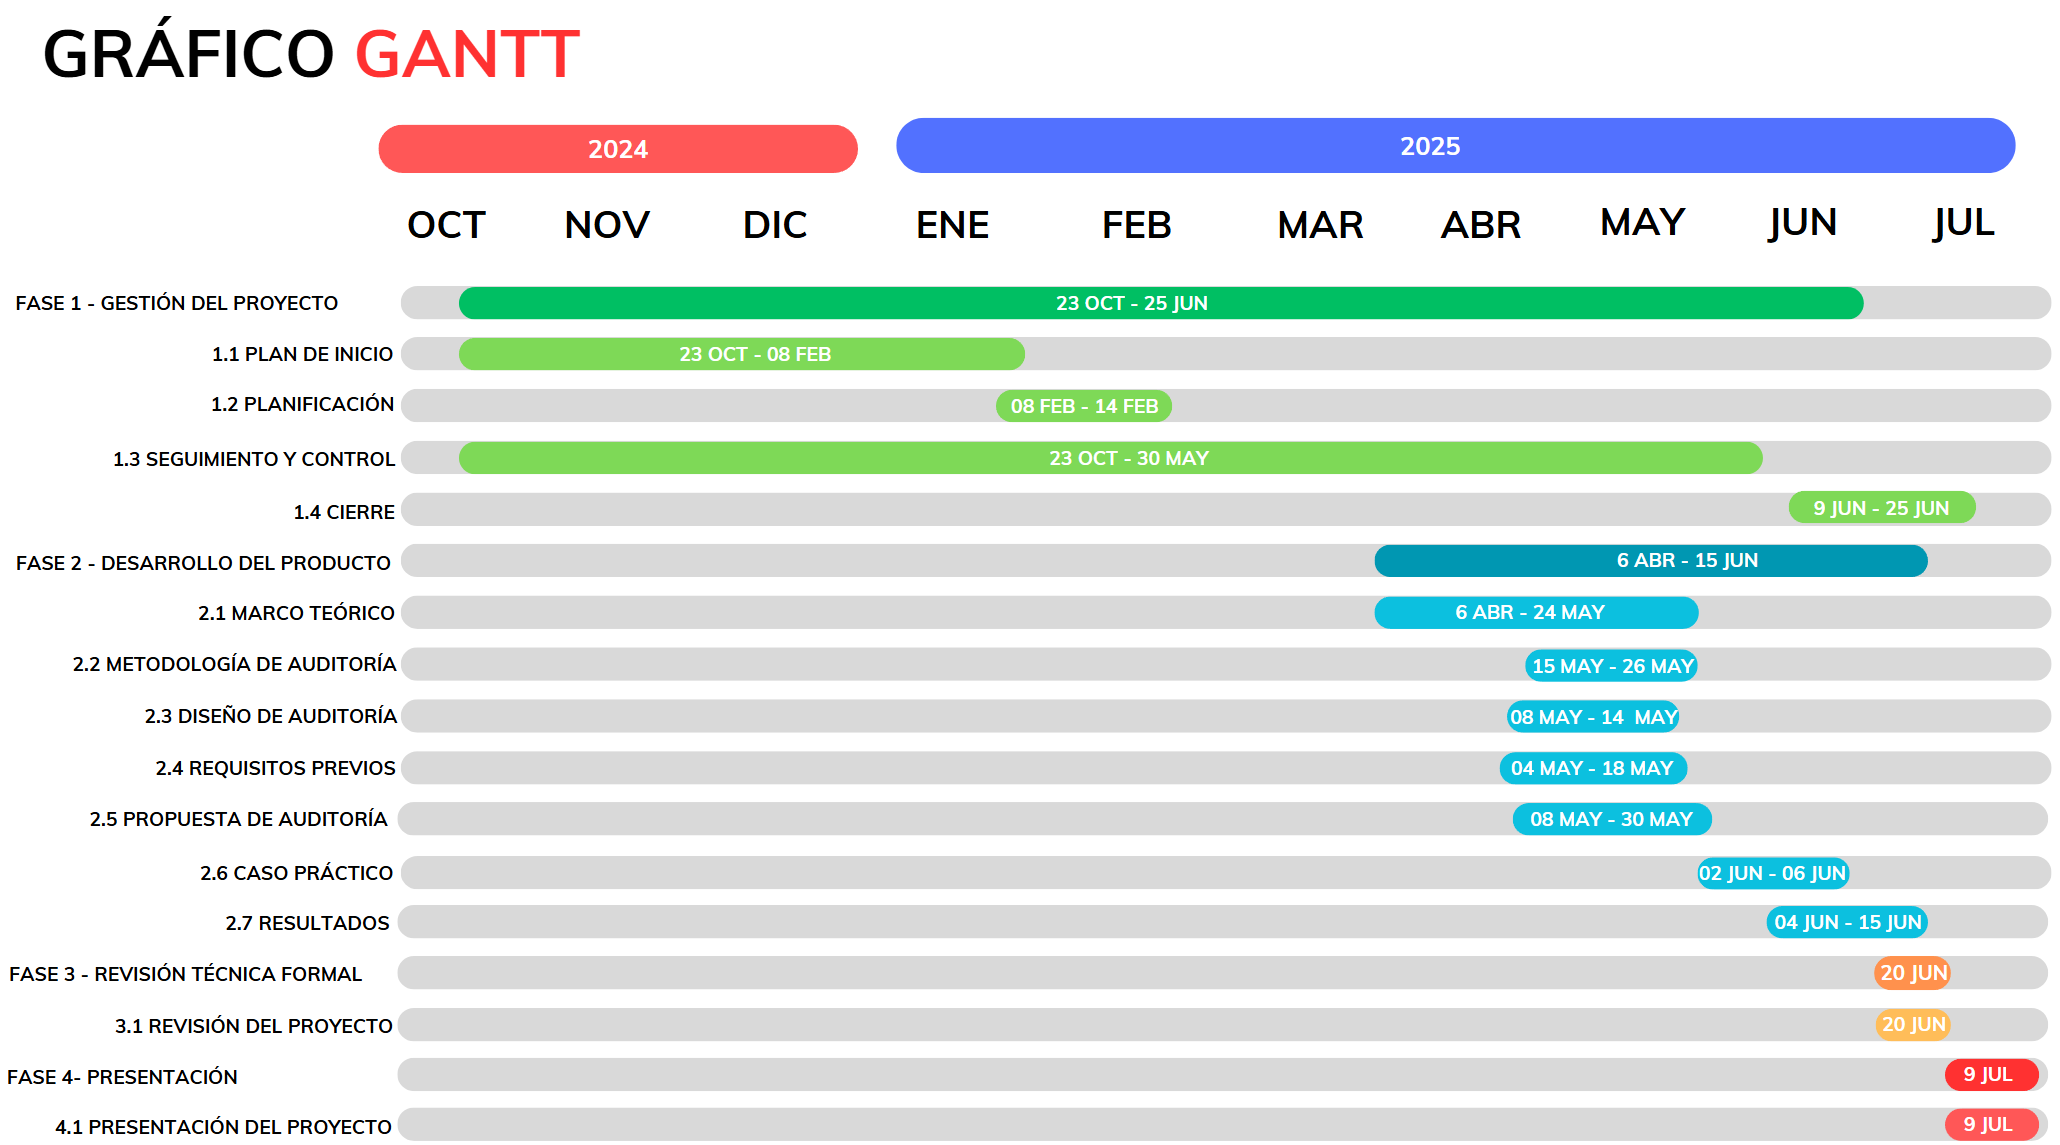
\includegraphics[width=24cm]{images/gant.png}
    \caption{Cronograma del proyecto. Fuente: Elaboración propia.}
    \label{fig:cronograma}
\end{figure}
\end{landscape}
\clearpage


\subsection{Roles y responsabilidades}
\par\vspace{0.5cm}

\begin{table}[H]
    \centering
    \caption{Distribución de roles y responsabilidades en el proyecto}
    \begin{tabular}{|c|c|}

        \hline
        \textbf{Rol} & \textbf{Responsabilidad} \\
        \hline
        Analista/Desarrollador (Alumno) & Planificación y redacción del documento \\
        \hline
        Analista/Desarrollador (Alumno) & Investigación y análisis de ciberseguridad en PYMEs \\
        \hline
        Analista/Desarrollador (Alumno) & Desarrollo del marco teórico \\
        \hline
        Analista/Desarrollador (Alumno) & Agrupación y redacción de requisitos previos para auditoría \\
        \hline
        Analista/Desarrollador (Alumno) & Identificación y documentación de normativas aplicables \\
        \hline
        Analista/Desarrollador (Alumno) & Creación de plan de auditoría propio \\
        \hline
        Analista/Desarrollador (Alumno) & Diseño de la metodología de auditoría \\
        \hline
        Analista/Desarrollador (Alumno) & Implementación práctica de la auditoría \\
        \hline
        Analista/Desarrollador (Alumno) & Ejecución del caso práctico \\
        \hline
        Analista/Desarrollador (Alumno) & Análisis de resultados y redacción del informe final \\
        \hline
        Jefe de proyecto (Tutor) & Asesoramiento en la selección del tema y enfoque del proyecto \\
        \hline
        Jefe de proyecto (Tutor) & Orientación y supervisión del trabajo del alumno \\
        \hline
        Jefe de proyecto (Tutor) & Organizar el desarrollo del caso práctico \\
        \hline
        Jefe de proyecto (Tutor) & Correcciones y evaluación del proyecto \\
        \hline
        Jefe de equipo (CTO de BeeHacker) & Proporcionar información técnica relevante y feedback \\
        \hline
        Jefe de equipo (CTO de BeeHacker) & Validación de la metodología y resultados del caso práctico \\
        \hline

    \end{tabular}
    \begin{flushleft}\centering
        \footnotesize \textbf{Fuente:} Elaboración propia
    \end{flushleft}    
    \label{tab:distribucion_roles}
\end{table}

\par\vspace{0.5cm}



\subsection{Recursos}
\par\vspace{0.5cm}

Los recursos necesarios para el desarrollo de la auditoría de ciberseguridad se dividen en tres categorías principales: recursos humanos, materiales y costos asociados. Cada una de estas categorías, se detalla en los siguientes apartados.
\par\vspace{0.5cm}

\subsubsection{Recursos Humanos}
\par\vspace{0.5cm}

En virtud del documento oficial de la Junta de Andalucía \cite{junta-perfiles}, se establecen los costes por hora de los perfiles profesionales necesarios para la realización del proyecto.
\par\vspace{0.5cm}

\begin{table}[H]
\caption{Recursos Humanos}
\centering
\renewcommand{\arraystretch}{1.5}
\begin{tabular}{|c|c|c|}
\hline
\textbf{Recurso} & \textbf{Tipo} & \textbf{Costo por Hora}  \\ \hline
Director de Proyecto & Trabajo & 63,75 €/h  \\ \hline
Jefe de Equipo & Trabajo & 53,55 €/h  \\ \hline
Analista & Trabajo & 47,17 €/h  \\ \hline
\end{tabular}
\begin{flushleft}\centering
    \footnotesize \textbf{Fuente:} Elaboración propia
\end{flushleft}   
\label{tab:recursos_humanos}
\end{table}



\subsubsection{Recursos Materiales}
\begin{table}[H]
\caption{Recursos Materiales}
\centering
\renewcommand{\arraystretch}{1.5}
\begin{tabular}{|c|c|c|c|c|}
\hline
\textbf{Recurso} & \textbf{Tipo} & \textbf{Costo Unitario} & \textbf{Unidades} & \textbf{Costo Total}  \\ \hline
Impresora & Material & €50,00 & 1& €50,00  \\ \hline
Disco Duro Externo & Material &  €60,00 &1& €60,00  \\ \hline
Pen Drive & Material & €20,00 & 1& €20,00  \\ \hline
Ordenador & Material & €600,00 & 1& €600,00  \\ \hline
Herramientas Hacking & Material & €500,00 & 1& €500,00  \\ \hline
\end{tabular}
\begin{flushleft}\centering
    \footnotesize \textbf{Fuente:} Elaboración propia
\end{flushleft}   
\label{tab:recursos_materiales}
\end{table}



\subsubsection{Costos Asociados}

\begin{table}[H]
\caption{Costos Asociados}
\centering
\renewcommand{\arraystretch}{1.5}
\begin{tabular}{|c|c|c|c|}
\hline
\textbf{Recurso} & \textbf{Tipo} & \textbf{Costo Total} & \textbf{Coste Estimado}  \\ \hline
Reserva de Contingencia & Costo & Variable & 1000€  \\ \hline
Licencias Software & Costo & Variable &  100€ \\ \hline
\end{tabular}
\begin{flushleft}\centering
    \footnotesize \textbf{Fuente:} Elaboración propia
\end{flushleft}   
\label{tab:costos_asociados}
\end{table}



\subsection{Estimación de Costes}
\par\vspace{0.5cm}

Considerando los recursos descritos anteriormente, se prevé que el \textbf{Analista} desempeñe un total de \textbf{300 horas de trabajo}, lo que supone un coste estimado de \underline{14.151 €}.  
\par\vspace{0.3cm}

En cuanto al \textbf{Director de Proyecto}, se estima una dedicación de \textbf{20 horas} centradas en tareas de corrección, revisión y supervisión general del proyecto, lo que representa un coste de \underline{1.275 €}.  
\par\vspace{0.3cm}

Respecto al \textbf{Jefe de Equipo}, se calcula un total de \textbf{10 horas} destinadas a la asistencia técnica y apoyo en el desarrollo de la auditoría, con un coste asociado de \underline{535,50 €}.  
\par\vspace{0.3cm}

Además, es necesario considerar los \textbf{costos adicionales asociados} al proyecto, entre los que destacan una \textbf{reserva de contingencia} de \underline{1.000 €} para posibles imprevistos y el coste de las \textbf{licencias de software} necesarias, estimado en 100 €, lo que suma un total de \underline{1.100 €}.  
\par\vspace{0.3cm}

En lo que respecta a los \textbf{recursos materiales}, se ha calculado un coste global de \underline{1230 €}, correspondiente a la adquisición de los elementos físicos indispensables para el desarrollo del trabajo.  
\par\vspace{0.3cm}

Este cálculo corresponde a una \textbf{duración estimada del proyecto de 4 meses}, durante los cuales se prevé que los profesionales involucrados realicen las tareas planificadas dentro de las horas estipuladas.  

\par\vspace{0.5cm}
\textbf{De esta manera, los costes totales estimados son los siguientes:}  

\begin{table}[H]
\caption{Resumen de costes del proyecto}
\centering
\renewcommand{\arraystretch}{1.5}
\begin{tabular}{|c|c|}
\hline
\textbf{Concepto} & \textbf{Monto (€)} \\ \hline
Recursos Humanos & 15.961,50 € \\ \hline
Recursos Materiales & 1230 € \\ \hline
Costos Asociados & 1.100 € \\ \hline
\textbf{Total Estimado} & \underline{\textbf{18.291,50 €}} \\ \hline
\end{tabular}
\begin{flushleft}\centering
    \footnotesize \textbf{Fuente:} Elaboración propia
\end{flushleft}   
\label{tab:resumen_costes}
\end{table}



\clearpage
\thispagestyle{nohead}









% -----------------------------------------------REQUISITOS FORMALES------------------------------------------------------------



\section{Requisitos formales}
\par\vspace{0.5cm}
Una vez definido el contexto general del proyecto y delimitado su alcance, se establecen los requisitos formales necesarios para la correcta redacción y desarrollo del trabajo, estructurados en una tabla.
\par\vspace{0.5cm}

Dicha tabla recoge, los principales requisitos identificados para el desarrollo del proyecto, agrupados en distintas categorías. Para cada requisito se indica su fuente 
o parte interesada, el objetivo específico al que contribuye dentro del proyecto, y el criterio que permitirá validar su cumplimiento.

\begin{landscape}
\begin{table}
\centering
\small
\begin{tabular}{|p{1cm}|p{6cm}|p{2.5cm}|p{2.7cm}|p{3.2cm}|p{4.9cm}|}
\hline
\textbf{ID} & \textbf{Requisito} & \textbf{Categoría} & \textbf{Fuente / Interesado} & \textbf{Objetivo(s) del Proyecto} & \textbf{Criterio(s) de Aceptación} \\
\hline
RF-01 & Los documentos deben extraerse de Google Scholar para su citación. & Documentación e información & Estudiante & Establecer un marco teórico riguroso & Referencias académicas verificables \\
\hline
RF-02 & Se recomienda utilizar publicaciones con una antigüedad no superior a 3 o 4 años. & Documentación e información & Tutor & Asegurar información actualizada & Año de publicación \\
\hline
RF-03 & Todos los documentos consultados se citarán en formato APA. & Documentación e información & Universidad & Cumplir formato académico & Revisión de estilo \\
\hline
RF-04 & Los documentos deben contener información relevante y actualizada sobre ciberseguridad en PYMEs. & Documentación e información & Estudiante & Fundamentos del trabajo & Relevancia del contenido \\
\hline
RF-05 & Elaborar una guía clara, comprensible y aplicable, orientada a perfiles no técnicos. & Documentación e información & Estudiante & Facilitar la adopción de buenas prácticas por parte de PYMEs & Guía redactada, revisada y publicada junto al informe \\
\hline
RF-06 & Estudiar y desarrollar los fundamentos teóricos de la ciberseguridad. & Marco teórico & Estudiante / Tutor & Fundamentar teóricamente el análisis posterior & Redacción clara y coherente del marco teórico \\
\hline
RF-07 & Las normativas deben ser oficiales y de libre acceso, proporcionadas por organismos reconocidos. & Normativas y certificaciones & Estudiante & Sostener la validez de la metodología & Fuentes oficiales citadas \\
\hline
RF-08 & La metodología debe seguir requerimientos oficiales de ciberseguridad. & Propuesta de metodología de la auditoría & Estándares & Proponer metodología válida & Alineación con normativas y metodologías reconocidas \\
\hline
RF-09 & Describir las implementaciones de hardware y software necesarias para proteger los sistemas. & Propuesta de metodología de la auditoría & Estudiante & Propuesta técnica clara & Herramientas identificadas y justificadas \\
\hline
RF-10 & Descripción del sistema auditado, incluyendo modelo y vulnerabilidades. & Sobre el caso práctico & Estudiante & Documentar el contexto práctico & Información técnica recopilada \\
\hline
RF-11 & Aplicación de la metodología en la PYME seleccionada. & Sobre el caso práctico & Estudiante & Validar la metodología propuesta & Aplicación práctica verificada \\
\hline
RF-12 & Detalle de las pruebas realizadas y los riesgos detectados. & Sobre el caso práctico & Estudiante & Identificar amenazas y vulnerabilidades & Resultados documentados de las pruebas \\
\hline
RF-13 & Redactar un informe final que contenga el análisis de riesgos, vulnerabilidades y propuestas de mejora. & Sobre el caso práctico & Estudiante & Sintetizar hallazgos y proponer soluciones & Informe estructurado y evaluado según criterios académicos \\
\hline
RF-14 & Incluir un apartado final con los resultados generales del TFG. & Resultados & Tutor / Universidad & Sintetizar conclusiones y validar el proceso & Sección de resultados redactada y bien estructurada \\
\hline
\end{tabular}
\caption{Requisitos formales del proyecto}
\label{tab:requisitos_formales}
\vspace{0.2cm}
\end{table}
\end{landscape}







\clearpage
\thispagestyle{nohead}


% -----------------------------------------------MARCO TEÓRICO------------------------------------------------------------

\section{Fundamentos teóricos para una auditoría de ciberseguridad en PYMEs}
\par\vspace{0.5cm}


El presente marco teórico tiene como objetivo establecer una base sólida sobre los principios fundamentales de la ciberseguridad aplicados al contexto de las pequeñas y medianas empresas (PYMEs). A lo largo del capítulo se abordarán los principales riesgos y amenazas que enfrentan estas organizaciones en el entorno digital, así como planes de mitigación que ofrecen estrategias prácticas para reducir su exposición a ciberataques.

\par\vspace{0.5cm}

Posteriormente, se detallan las buenas prácticas recomendadas, distinguiendo entre aquellas que deben adoptar internamente las PYMEs y las que se aplican durante las auditorías de seguridad, contribuyendo así a un enfoque integral desde ambas perspectivas.

\par\vspace{0.5cm}

A continuación, se exponen las normativas nacionales y europeas más relevantes, que definen el marco legal y regulatorio que debe ser respetado por las PYMEs para asegurar la protección de sus activos 
digitales. Además, se presentan los estándares y metodologías de auditoría más reconocidos internacionalmente, para basar la propuesta de auditoría en algunos de ellos.

\par\vspace{0.5cm}


Finalmente, se describe las herramientas más usadas en auditorías de ciberseguridad y se dedica un último apartado para orientar a quienes deseen especializarse en ciberseguridad ofensiva, incluyendo las certificaciones profesionales más relevantes, organizadas por nivel de dificultad, que permiten diseñar un itinerario formativo progresivo y efectivo.
\par\vspace{0.5cm}

Esta exposición teórica sentará las bases para el desarrollo posterior de una propuesta concreta de auditoría de ciberseguridad adaptada a las necesidades específicas de las PYMEs.








\par\vspace{0.5cm}







\subsection{Principales amenazas y riesgos para PYMEs}
\par\vspace{0.5cm}

La ciberseguridad representa un desafío importante para muchas pequeñas y medianas empresas españolas. Según el informe de Hiscox \cite{hiscox}, cerca del 50\% de las empresas en España sufrió algún tipo de ciberataque en 2023. Las PYMEs, en particular, son cada vez más objetivo de estos ataques debido a su limitada preparación en ciberseguridad. De hecho, solo el 61\% de las empresas con menos de 250 empleados se sienten seguras de su preparación en este sector. 
\par\vspace{0.5cm}

El Instituto Nacional de Ciberseguridad (INCIBE) registró en 2022 un total de 118.000 incidentes de ciberseguridad, un 9\% más que el año anterior \cite{incibe2023}. Una gran parte de estos incidentes afectaron a pequeñas y medianas empresas, y uno de cada tres se trató de una filtración de datos.
\par\vspace{0.5cm}

Aunque cada vez más PYMEs aumentan sus presupuestos en ciberseguridad y colaboran con empresas especializadas, muchas todavía optan por contratar a otras empresas especializadas para que se encarguen de gestionar sus servicios de ciberseguridad, 
por falta de personal y recursos internos. Esta 
externalización, debe complementarse con una adecuada cultura interna de seguridad, especialmente mediante la formación del personal.
\par\vspace{0.5cm}

Según PwC España \cite{pwc}, el 86\% de las organizaciones considera que sus empleados carecen de una cultura de ciberseguridad adecuada, lo que pone en pie la necesidad urgente de concienciación.
\par\vspace{0.5cm}

Entre las principales ciberamenazas que afectan a las PYMEs según la empresa de Software Treyder \cite{treyder} se encuentran:

\begin{itemize}
    \item \textbf{Malware:}  
    El término engloba todo tipo de software malicioso diseñado para infiltrarse o dañar un sistema sin el consentimiento del usuario. Incluye virus, troyanos, spyware y especialmente ransomware, que cifra los datos del sistema y exige un rescate económico para su recuperación. Las PYMEs suelen ser víctimas de malware distribuido por correos adjuntos infectados o a través de enlaces maliciosos en páginas aparentemente legítimas. Además del daño económico, el malware puede provocar la pérdida permanente de datos, el control remoto de equipos y el espionaje corporativo.
\end{itemize}

\vspace{0.5cm}

La relevancia del malware como una de las principales ciberamenazas se refleja claramente en su evolución histórica. Tal y como muestra el informe de AV-TEST, la cantidad total de software malicioso (malware) y aplicaciones potencialmente no deseadas (PUA) ha experimentado un crecimiento exponencial en las últimas décadas, superando en 2024 los 1.500 millones de muestras registradas a nivel mundial. Este aumento constante evidencia que las amenazas digitales siguen sofisticándose y expandiéndose, afectando por igual a grandes empresas y a pequeñas organizaciones como las PYMEs.

\vspace{0.3cm}

\begin{figure}[H]
    \centering
    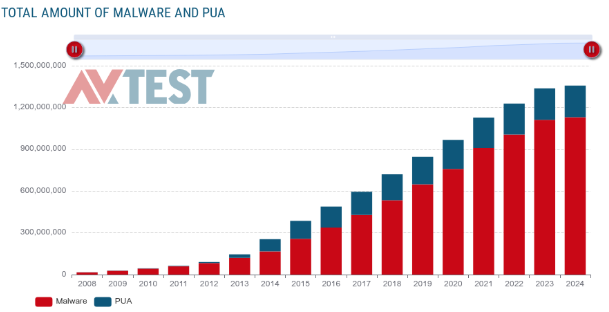
\includegraphics[width=0.95\textwidth]{images/malware.png}
    \caption{Evolución histórica de la cantidad total de malware y PUA a nivel mundial. Fuente: AVTEST \cite{avtest}.}
\end{figure}

\vspace{0.5cm}

Aparte del malware, existen otras amenazas igualmente relevantes para las PYMEs como se expone en Taipe-Yanez y Pallo-Tulmo (2024) \cite{vuln}, como son: 
\par\vspace{0.5cm}

\begin{itemize}
    \item \textbf{Phishing:}  
    Consiste en técnicas de suplantación de identidad para engañar y obtener datos confidenciales, como contraseñas, credenciales bancarias o información sensible de clientes. Suele realizarse mediante correos electrónicos o mensajes falsificados que imitan a bancos, plataformas de pago o servicios tecnológicos conocidos. En las PYMEs, donde el nivel de concienciación en ciberseguridad suele ser limitado, el phishing representa una puerta de entrada frecuente a ataques más complejos, como el acceso remoto a sistemas o la instalación de malware. 
    \vspace{0.3cm}

    \item \textbf{Ataques de denegación de servicio (DDoS):}  
    Este tipo de ataque busca hacer que los servidores, aplicaciones o sitios web de una empresa queden inoperativos mediante el envío masivo de peticiones falsas. Se trata de una sobrecarga intencionada de los recursos tecnológicos de la organización, que impide el funcionamiento normal de servicios clave. Aunque muchas veces se asocian a grandes empresas, las PYMEs también son objetivo, especialmente si ofrecen servicios digitales o tiendas online. Un DDoS puede paralizar las operaciones durante horas o días, con pérdidas económicas importantes y daño reputacional. 
    \vspace{0.3cm}

    \item \textbf{Brechas de datos:}  
    Ocurren cuando un atacante consigue acceder sin autorización a bases de datos internas, habitualmente mediante credenciales robadas, vulnerabilidades no parcheadas o ingeniería social. Estas brechas pueden afectar a información crítica como datos de clientes, contraseñas, información financiera o planes estratégicos. Para una PYME, una brecha de datos no solo puede suponer sanciones legales (por ejemplo, si no cumple con el Reglamento General de Protección de Datos (RGPD)), sino también pérdida de confianza por parte de clientes y socios. 
    \vspace{0.3cm}

    \item \textbf{Errores de configuración:}  
    Son fallos humanos o técnicos al configurar correctamente sistemas, redes o aplicaciones. Por ejemplo, dejar puertos abiertos innecesarios, permitir contraseñas por defecto, o no establecer permisos adecuados. Estos errores abren puertas invisibles a los ciberatacantes y son especialmente comunes en entornos donde no existe un departamento de TI dedicado. La falta de mantenimiento o revisión de estas configuraciones puede convertir una infraestructura aparentemente segura en un objetivo fácil.

\end{itemize}

\par\vspace{0.5cm}
Además de los vectores de ataque mencionados anteriormente, es importante considerar ciertos \textbf{riesgos estructurales} que afectan de manera particular a las PYMEs, aumentando su exposición frente a ciberataques. Según la empresa  de seguridad digital GlobalSign, estos riesgos incluyen factores internos y operativos que suelen pasarse por alto en organizaciones de menor tamaño \cite{toms2021}. 
\begin{itemize}
  \item \textbf{Falta de recursos de seguridad:} Muchas pequeñas empresas no cuentan con personal especializado en ciberseguridad (como un CISO o un técnico en protección de datos), lo que dificulta la detección y respuesta ante incidentes.
  \item \textbf{Presupuestos limitados:} La inversión en ciberseguridad suele ser muy pobre frente a otras prioridades de negocio, lo que impide implementar soluciones de protección efectivas o actualizadas.
  \item \textbf{Falta de diseño seguro desde el inicio:} Al haber sido creadas por expertos en su sector y no por especialistas en tecnología, muchas PYMEs han desarrollado sus sistemas sin tener en cuenta principios de seguridad por defecto.
  \item \textbf{Ausencia de fondos de emergencia:} La falta de capacidad económica para hacer frente a pagos por rescates o pérdidas prolongadas de ingresos hace que las consecuencias de un ciberataque sean especialmente devastadoras.
  \item \textbf{Impacto operativo total ante incidentes graves:} Un ciberataque que provoque una filtración o la caída de sistemas puede detener completamente la actividad del negocio, ya que las PYMEs no suelen tener infraestructuras de respaldo.
\end{itemize}

\par\vspace{0.5cm}
Estos factores, sumados a una falsa sensación de anonimato (“somos demasiado pequeños para que nos ataquen”), aumentan considerablemente el riesgo de que las PYMEs se conviertan en blancos frecuentes y exitosos de los ciberdelincuentes. 
Implementar medidas preventivas y desarrollar una cultura de seguridad sólida resulta crucial para garantizar su continuidad. 

\par\vspace{0.5cm}

Finalmente, para ilustrar en tiempo real la magnitud y frecuencia global de estos ataques y reforzar la importancia de adoptar medidas de seguridad, puede consultarse el mapa 
interactivo donde se muestran los ciberataques que se acontecen en tiempo real proporcionado por Fortinet \cite{fortinet}. 

\begin{figure}[H]
    \centering
    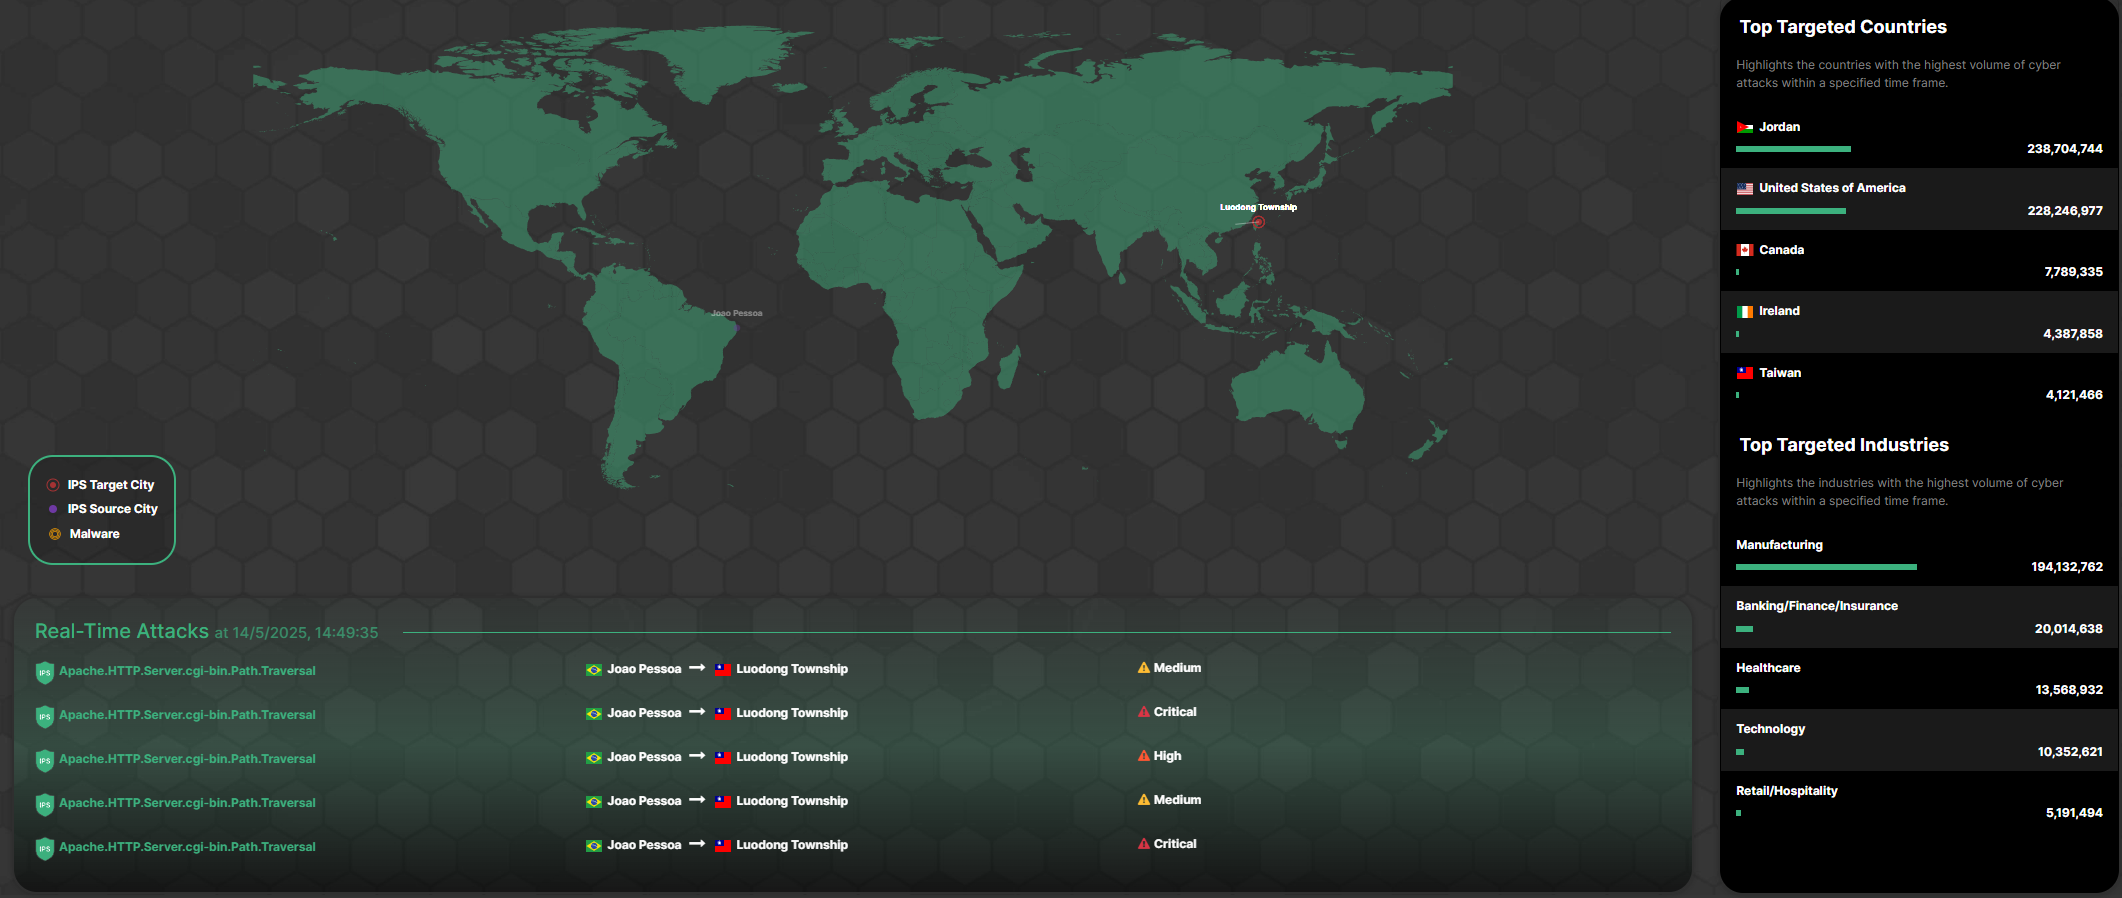
\includegraphics[width=\textwidth]{images/mapa.png}
    \caption{Mapa global de ciberamenazas en tiempo real. Fuente: Fortinet \cite{fortinet}.}
    \label{fig:mapa-fortiguard}
\end{figure}
\par\vspace{0.5cm}

\subsection{Planes de Mitigación}
\par\vspace{0.5cm}

Como destacan Viteri-Hernández y Avila-Pesantez en su revisión sistemática sobre seguridad en redes de proveedores de servicios de Internet \cite{mitigacion}, reducir los riesgos derivados de incidentes de ciberseguridad requiere implementar planes de mitigación efectivos, que incluyan medidas tanto técnicas como organizativas. Entre las principales técnicas destacan el uso de barreras preventivas como \textbf{firewalls y filtros de red}, el control proactivo del tráfico mediante \textbf{monitoreo continuo} y la adopción de mecanismos de \textbf{autenticación y control de acceso robustos}, que permiten proteger adecuadamente los recursos sensibles.
\par\vspace{0.5cm}

Asimismo, es crucial integrar estrategias orientadas a fortalecer la cultura de ciberseguridad dentro de la organización mediante \textbf{programas continuos de concienciación y formación del personal}, así como establecer mecanismos sistemáticos para la \textbf{gestión de vulnerabilidades}, aplicación periódica de \textbf{actualizaciones y parches}, y asegurar la confidencialidad mediante el \textbf{cifrado del tráfico de datos}.
\par\vspace{0.5cm}

Finalmente, la planificación debe considerar también la preparación frente a incidentes mediante la implementación de procedimientos eficaces de \textbf{respaldo y recuperación de información} y fomentar una cooperación activa con la \textbf{comunidad de ciberseguridad} para enfrentar eficazmente amenazas emergentes.
\par\vspace{0.5cm}

En la siguiente tabla se resumen las principales medidas de mitigación recomendadas, junto con sus características y efectividad:
\par\vspace{0.5cm}

\begin{table}[H]
    \centering
    \caption{Medidas de mitigación y su efectividad.}
    \begin{tabular}{p{4.5cm} p{10cm}}
    \toprule
    \textbf{Medida de mitigación} & \textbf{Características} \\
    \hline
    Firewalls y filtros de red & Establecen barreras de protección, controlan el tráfico y bloquean accesos no autorizados. Efectivos ante intrusiones externas. \\
    \bottomrule
    Monitoreo de red continuo & Permite la detección temprana de comportamientos anómalos y actividades sospechosas para una respuesta rápida. \\
    \bottomrule
    Protección contra DDoS & Mitiga ataques de denegación de servicio distribuido, asegurando la continuidad operativa. \\
    \bottomrule
    Actualizaciones y parches & Mantiene el software actualizado, cerrando vulnerabilidades conocidas y reduciendo el riesgo de explotación. \\
    \bottomrule
    Autenticación y control de acceso & Implementa verificación de identidad y restricciones de acceso a recursos sensibles, previniendo accesos no autorizados. \\
    \bottomrule
    Cifrado de tráfico & Protege la confidencialidad de los datos durante su transmisión entre servidores y usuarios. \\
    \bottomrule
    Segmentación de red & Divide la red en zonas aisladas para limitar la propagación de amenazas internas. \\
    \bottomrule
    Gestión de vulnerabilidades & Identifica y corrige debilidades de forma proactiva, fortaleciendo la postura de seguridad. \\
    \bottomrule
    Educación en ciberseguridad & Capacita al personal en buenas prácticas y prevención de ataques como la ingeniería social. \\
    \bottomrule
    Políticas de seguridad robustas & Define protocolos, responsabilidades y buenas prácticas para fomentar una cultura de seguridad. \\
    \bottomrule
    Respaldo y recuperación de datos & Garantiza la disponibilidad y restauración ante pérdida de datos o ciberataques. \\
    \bottomrule
    Colaboración con la comunidad de ciberseguridad & Facilita el intercambio de información y estrategias para enfrentar amenazas comunes. \\
    \bottomrule
    \end{tabular}
    \vspace{0.5em}
    \begin{flushleft}
    \footnotesize \textbf{Fuente:} EXPLORACIÓN INTEGRAL DE LA SEGURIDAD EN REDES DE PROVEEDORES DE SERVICIOS DE INTERNET \cite{mitigacion}
    \end{flushleft}
    \label{tab:medidas_mitigacion}
\end{table}
\par\vspace{0.5cm}

\subsection{Buenas prácticas}
\par\vspace{0.5cm}
Las buenas prácticas en el ámbito de la ciberseguridad constituyen un conjunto de acciones, políticas y medidas preventivas que buscan minimizar riesgos, proteger la información y garantizar la continuidad operativa ante posibles amenazas. En este apartado se diferenciarán dos perspectivas clave: por un lado, las buenas prácticas que una PYME debe implementar de forma interna para fortalecer su seguridad digital; y por otro, aquellas prácticas recomendadas y seguidas durante las auditorías de ciberseguridad, las cuales permiten evaluar el estado real de la infraestructura tecnológica y proponer mejoras efectivas.
\par\vspace{0.5cm}

\subsubsection{Buenas prácticas en PYMES}
\par\vspace{0.5cm}

La ciberseguridad en pequeñas y medianas empresas requiere un enfoque integral que combine herramientas, políticas, concienciación y planificación estratégica. Una única medida no es suficiente para garantizar la protección frente a las amenazas actuales. A continuación, se detallan algunas de las buenas prácticas más relevantes que una PYME debe adoptar para construir un entorno digital más seguro, según las recomendaciones de expertos \cite{toms2021}:

\begin{itemize}
    
    \item \textbf{Documentación de procesos y protocolos:}  
    Muchas PYMEs asignan a una sola persona la responsabilidad de la configuración y gestión de la seguridad informática. Sin embargo, esto supone un riesgo si esa persona abandona la empresa, ya que el conocimiento no queda registrado. Documentar todos los procesos, configuraciones y políticas de seguridad permite mantener la continuidad operativa, facilita auditorías internas y evita que la salida de personal clave comprometa la seguridad.

    \item \textbf{Contraseñas seguras y autenticación multifactorial (MFA):}  
    El uso de contraseñas débiles es una de las principales vulnerabilidades explotadas por los atacantes. Se recomienda utilizar contraseñas largas (mínimo 12 caracteres), 
    con combinación de letras, números y símbolos especiales. Además, es esencial implementar mecanismos de autenticación de doble factor (por ejemplo, mediante contraseña y huella dactilar, o código de un solo uso vía SMS), lo que añade una capa adicional de protección frente a accesos no autorizados.

    \item \textbf{Formación continua de los empleados:}  
    Los empleados suelen ser tanto la primera como la última línea de defensa ante ciberataques. Sin una formación adecuada, es más probable que caigan en fraudes por correo electrónico, 
    enlaces maliciosos o campañas de phishing dirigidas. Las PYMEs deben establecer programas de concienciación en ciberseguridad que incluyan formación sobre detección de amenazas, políticas de uso de dispositivos personales, buenas prácticas en navegación, y respuesta ante incidentes.

    \item \textbf{Enfoque de seguridad por capas (defensa en profundidad):}  
    La protección de los sistemas debe estar basada en múltiples niveles de seguridad que actúen de forma coordinada. Entre las medidas recomendadas se incluyen: 
    antivirus y antispyware actualizados, configuración adecuada del firewall, control de accesos, cifrado de los datos en tránsito y en reposo, y uso de firmas digitales para garantizar la integridad de los documentos. Esta arquitectura de defensa en profundidad mejora la resiliencia frente a ataques dirigidos o automatizados.

    \item \textbf{Copias de seguridad regulares y distribuidas:}  
    Las copias de seguridad son fundamentales para asegurar la recuperación de datos tras incidentes como ransomware, fallos de hardware o errores humanos. Se recomienda realizar copias frecuentes, almacenarlas en diferentes ubicaciones (local, nube o dispositivos externos), y verificar periódicamente que pueden restaurarse correctamente. Esta práctica sencilla puede marcar la diferencia entre la continuidad del negocio o la pérdida irreversible de información crítica.

\end{itemize}
\par\vspace{0.5cm}

\subsubsection{Buenas prácticas en auditorías de ciberseguridad}
\par\vspace{0.5cm}

Las auditorías son procesos estructurados que permiten evaluar el estado de la seguridad informática de una organización. 
Para que sean eficaces, deben llevarse a cabo bajo un conjunto de buenas prácticas que garanticen no solo la calidad técnica del análisis, sino también la ética profesional, 
la trazabilidad de los hallazgos y la aplicabilidad de las recomendaciones. Seguidamente, se describen las principales buenas prácticas que deben seguirse durante una auditoría de ciberseguridad:

\begin{itemize}

    \item \textbf{Definición clara del alcance:}  
    Antes de iniciar cualquier auditoría, es fundamental delimitar qué sistemas, redes, aplicaciones, ubicaciones y personas serán objeto de evaluación. Un alcance bien definido evita malentendidos, asegura que los recursos estén disponibles y permite centrar los esfuerzos en los activos más críticos.

    \item \textbf{Formalización mediante acuerdos previos:}  
    Toda auditoría debe comenzar con la firma de acuerdos de confidencialidad (NDA) y documentos de autorización por parte de la empresa auditada. Esto garantiza que el proceso se realice dentro del marco legal y ético, y protege tanto al auditor como a la organización.

    \item \textbf{Aplicación de metodologías reconocidas:}  
    Las auditorías deben basarse en estándares y marcos metodológicos ampliamente aceptados, como PTES (Penetration Testing Execution Standard), OSSTMM (Open Source Security Testing Methodology Manual), o las guías del NIST (por ejemplo, SP 800-115). Esto asegura un enfoque sistemático, riguroso y alineado con las mejores prácticas internacionales.

    \item \textbf{Uso controlado de herramientas especializadas:}  
    El empleo de herramientas debe realizarse de forma responsable, en entornos previamente autorizados, y con medidas que minimicen posibles interrupciones del servicio. Se recomienda documentar cada herramienta utilizada, junto con su propósito y los resultados obtenidos.

    \item \textbf{Documentación exhaustiva de hallazgos:}  
    Cada vulnerabilidad o debilidad detectada debe registrarse con claridad, incluyendo una descripción técnica, nivel de riesgo, posible impacto y evidencias que lo respalden. Esta documentación será esencial para la elaboración del informe final.

    \item \textbf{Informe técnico y ejecutivo:}  
    El resultado de la auditoría debe presentarse en dos formatos: uno técnico, dirigido al personal de sistemas, y otro ejecutivo, accesible para la dirección de la empresa. Ambos informes deben incluir un plan de acción priorizado y recomendaciones específicas y viables.

    \item \textbf{Propuesta de mejora continua:}  
    La auditoría no debe verse como un fin en sí misma, sino como parte de un proceso de mejora continua. Es importante que el informe incluya sugerencias para establecer controles recurrentes, políticas de seguridad y mecanismos de revisión periódica.

    \item \textbf{Ética profesional y confidencialidad:}  
    Durante todo el proceso, el equipo auditor debe actuar con responsabilidad, integridad y confidencialidad. Cualquier hallazgo crítico debe comunicarse de inmediato a los responsables de seguridad de la organización, sin esperar al informe final.

\end{itemize}
\par\vspace{0.5cm}

\subsection{Marco Regulatorio y Metodológico en Ciberseguridad}
\par\vspace{0.5cm}

La ciberseguridad se ha consolidado como un pilar esencial para la protección de los activos digitales, tanto en el ámbito público como privado. En un entorno cada vez más digitalizado y expuesto a riesgos tecnológicos, contar con un marco normativo sólido y con metodologías contrastadas resulta imprescindible para garantizar la integridad, confidencialidad y disponibilidad de la información. Esta sección presenta los principales organismos encargados de regular y supervisar la ciberseguridad en España, así como las metodologías empleadas en auditorías y evaluaciones técnicas. Comprender este marco es clave para aplicar buenas prácticas y actuar conforme a los estándares exigidos a nivel nacional y europeo.
\par\vspace{0.5cm}

\subsubsection{Organismos Reguladores en Ciberseguridad}
\par\vspace{0.5cm}

En España, diversos organismos desempeñan un papel clave en la regulación, supervisión y fomento de la ciberseguridad. Entre ellos destacan:
\par\vspace{0.5cm}

\subsection*{Instituto Nacional de Ciberseguridad (INCIBE)}
 Es una entidad pública de referencia nacional en materia de ciberseguridad, vinculada al Ministerio de Asuntos Económicos 
y Transformación Digital, a través de la Secretaría de Estado de Digitalización e Inteligencia Artificial. INCIBE desempeña un papel esencial en el impulso de la 
ciberseguridad en España, especialmente orientado al sector empresarial. \cite{incibe}

\par\vspace{0.5cm}

Los pilares fundamentales sobre los que se estructura la actividad de esta organización son:
\begin{itemize}
\item \textbf{Protección}, \textbf{Prevención} y \textbf{Reacción} ante incidentes de ciberseguridad.
\item \textbf{Investigación} y desarrollo de tecnologías aplicadas a la seguridad.
\item \textbf{Generación de inteligencia} para anticipar amenazas y vulnerabilidades.
\item \textbf{Mejora de servicios} y capacidades en ciberseguridad.
\item \textbf{Colaboración activa} con entidades públicas y privadas para reforzar el ecosistema de seguridad digital.
\end{itemize}

\begin{figure}[H]
\centering
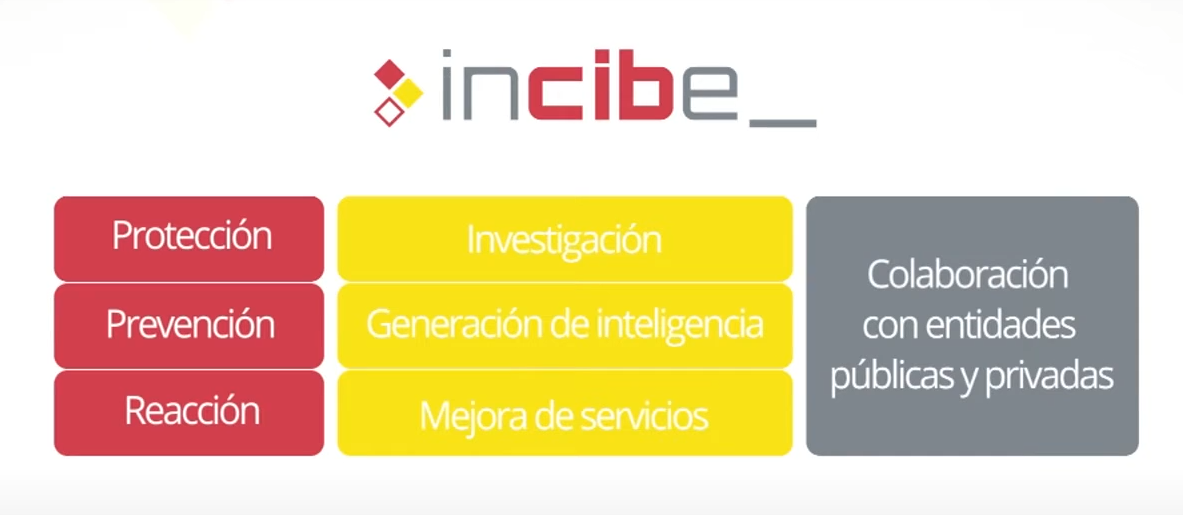
\includegraphics[width=10cm]{images/incibe.png}
\caption{Pilares fundamentales de INCIBE. Fuente: INCIBE \cite{incibe}.}
\label{fig:incibe-pilares}
\end{figure}

\par\vspace{0.5cm}
\subsection*{Centro Nacional de Inteligencia (CNI)}

Es el organismo responsable de proporcionar al Gobierno información y análisis necesarios para prevenir y contrarrestar cualquier amenaza contra la soberanía, integridad y seguridad nacional, incluyendo las de naturaleza cibernética. A través de estrategias de inteligencia y cooperación con otras agencias, tanto nacionales como internacionales, el CNI participa activamente en la defensa frente a ciberamenazas que puedan poner en riesgo los intereses fundamentales del país. \cite{cni}
\par\vspace{0.5cm}

\subsection*{Centro Criptológico Nacional (CCN-CERT)}

Forma parte del Centro Nacional de Inteligencia (CNI) y actúa como el equipo de respuesta a incidentes de ciberseguridad para las administraciones públicas y entidades que gestionan infraestructuras críticas. Su función principal es prevenir, detectar y responder a ciberamenazas que puedan comprometer los sistemas del sector público español. Además, el CCN-CERT emite guías técnicas, alertas, buenas prácticas y herramientas diseñadas para aumentar la capacidad defensiva del Estado ante ciberincidentes. \cite{ccncert}



\par\vspace{0.5cm}

\subsection*{Agencia Española de Protección de Datos (AEPD)}

Autoridad independiente encargada de supervisar el cumplimiento del Reglamento General de Protección de Datos (RGPD) y la Ley Orgánica 3/2018 (LOPD-GDD), además de ofrecer orientación y recursos a organizaciones para gestionar datos personales de manera segura \cite{aepd}.
\par\vspace{0.5cm}


\subsubsection{Otros Organismos Internacionales}

\par\vspace{0.5cm}

Además, existen organismos internacionales relevantes cuya influencia en ciberseguridad tiene alcance global, incluidos España y Europa:
\par\vspace{0.5cm}




\subsection*{National Institute of Standards and Technology (NIST)}

Es una agencia federal estadounidense que desarrolla estándares, directrices y mejores prácticas en ciberseguridad. Reconocido a nivel internacional, el NIST ha establecido marcos de referencia ampliamente adoptados por organizaciones públicas y privadas para gestionar eficazmente los riesgos asociados a la seguridad digital \cite{nist}.
\par\vspace{0.5cm}

Uno de sus marcos más influyentes es el \textbf{NIST Cybersecurity Framework (CSF)}, una guía estructurada para que cualquier organización pueda identificar, proteger, detectar, responder y recuperar frente a ciberincidentes. Este modelo se basa en cinco funciones clave:
\begin{enumerate}
\item \textbf{Identificar (Identify)}: comprender el entorno organizativo, sus activos y riesgos para establecer un enfoque de gestión de seguridad adecuado.
\item \textbf{Proteger (Protect)}: desarrollar y aplicar medidas de salvaguarda para limitar o contener el impacto de un incidente.
\item \textbf{Detectar (Detect)}: implementar actividades que permitan identificar de forma oportuna la ocurrencia de eventos de ciberseguridad.
\item \textbf{Responder (Respond)}: tomar medidas para contener el impacto de un evento detectado, mediante planes, comunicaciones, análisis y mitigación.
\item \textbf{Recuperar (Recover)}: restaurar las capacidades afectadas para garantizar la continuidad del negocio tras un incidente.
\end{enumerate}

\begin{figure}[H]
\centering
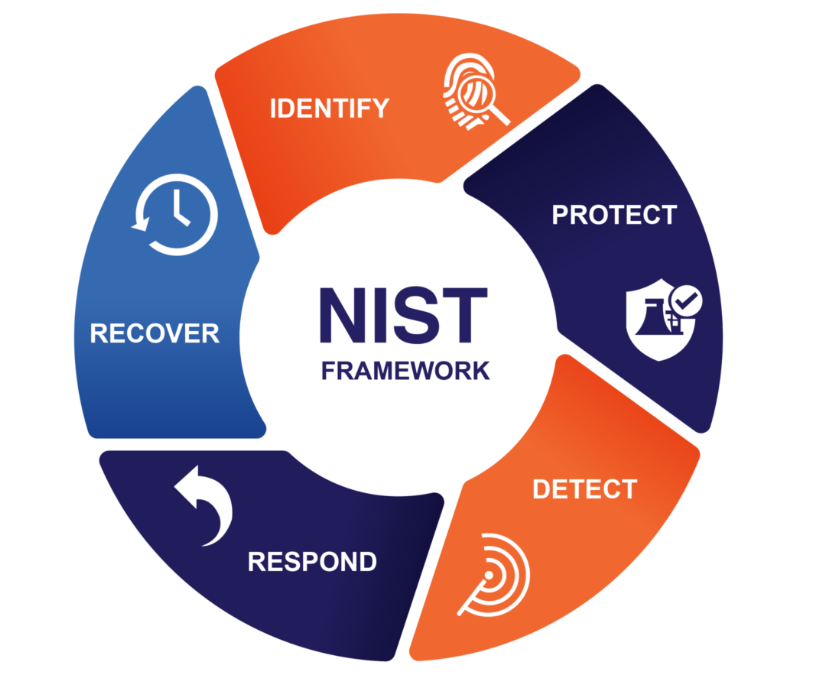
\includegraphics[width=7cm]{images/nist_framework.png}
\caption{Funciones del Marco de Ciberseguridad de NIST. Fuente: DEVICE42 Company \cite{device42}.}
\label{fig:nist-framework}
\end{figure}

Este enfoque es adaptable y escalable, y ha sido adoptado no solo en Estados Unidos, sino también en muchos países como referencia para desarrollar políticas nacionales de ciberseguridad y estándares corporativos.

\par\vspace{0.5cm}

Otra pieza fundamental desarrollada por esta entidad es la \textbf{serie NIST Special Publications 800 (SP 800)}, que comprende más de 130 documentos gratuitos disponibles para descarga, en los que se describen políticas, procedimientos y directrices sobre ciberseguridad, evaluaciones de riesgos, controles técnicos y auditoría. Esta colección se considera una de las fuentes más completas y detalladas en materia de seguridad de la información. \cite{nistsp}
\par\vspace{0.5cm}

Dentro de esta serie, se encuentran guías ampliamente reconocidas como la NIST SP 800-53 (controles de seguridad y privacidad) o la SP 800-115 (metodología para pruebas técnicas de seguridad). En capítulos posteriores, se seleccionarán y adaptarán varias de estas metodologías como base para diseñar nuestra propia propuesta de auditoría adaptada al contexto de PYMEs.


\par\vspace{0.5cm}



\subsection*{SANS Institute (SysAdmin, Audit, Networking, and Security Institute)}
Es una de las organizaciones más reconocidas a nivel mundial en el ámbito de la ciberseguridad. 
Su objetivo principal es proporcionar formación avanzada y especializada en seguridad informática a profesionales, empresas y organismos públicos. \cite{sans}
\par\vspace{0.5cm}

Además de sus programas de formación, SANS es responsable de desarrollar y mantener recursos ampliamente utilizados en la industria, como el Top 20 Critical Security Controls y el proyecto GIAC (Global Information Assurance Certification). GIAC es un sistema de certificación reconocido internacionalmente que valida las competencias técnicas en múltiples especialidades de ciberseguridad, desde pentesting hasta auditoría o administración de sistemas seguros. \cite{sanscert}
\par\vspace{0.5cm}


\begin{table}[H]
\centering
\caption{Certificaciones GIAC ofrecidas por SANS y sus áreas de especialización}
\begin{tabular}{|l|l|}
\hline
\textbf{Área de especialización} & \textbf{Certificación GIAC} \\
\hline
Seguridad general & GSEC (Security Essentials) \\
Pentesting y hacking ético & GPEN (Penetration Tester), GXPN (Exploit Researcher) \\
Respuesta ante incidentes & GCIH (Incident Handler) \\
Análisis forense & GCFA (Forensic Analyst), GCFE (Forensic Examiner) \\
Administración de sistemas seguros & GCWN (Windows), GCUX (Unix/Linux) \\
Gestión de riesgos y auditoría & GSNA (Systems and Network Auditor), \\
&GRCP (Risk and Compliance)\\
Defensa de redes y sistemas & GCIA (Intrusion Analyst), GCCC (Critical Controls) \\
\hline
\end{tabular}
\begin{flushleft}
\footnotesize \textbf{Fuente:} Red Team Operations Certifications. \cite{sanscert}

\end{flushleft}
\label{tab:giac-certificaciones}
\end{table}

\subsubsection{Normativas y Estándares Aplicables}
\par\vspace{0.5cm}

En el contexto nacional y europeo, las normativas más relevantes en ciberseguridad aplicables especialmente a PYMEs son:
\par\vspace{0.5cm}

\subsection*{Esquema Nacional de Seguridad (ENS)}

Regulado por el Real Decreto 311/2022, el Esquema Nacional de Seguridad (ENS) establece los principios básicos y los requisitos mínimos necesarios para una adecuada protección de la información manejada por medios electrónicos. Está dirigido tanto a las administraciones públicas como a aquellas entidades del sector privado que colaboran con el sector público.
\par\vspace{0.5cm}

Su objetivo principal es garantizar el acceso, la confidencialidad, la integridad, la trazabilidad, la autenticidad y la conservación de los datos. Para ello, el ENS define tres niveles de seguridad (bajo, medio y alto) y obliga a realizar un análisis de riesgos para aplicar las medidas correspondientes. 
El marco del ENS también contempla la implantación de una política de seguridad y la designación de responsables de seguridad en las organizaciones \cite{boe_ens}.
\par\vspace{0.5cm}

\subsection*{Reglamento General de Protección de Datos (RGPD)}

Es una normativa implementada en la Unión Europea que regula la legislación sobre protección de datos en todos los Estados miembros. 
Su aplicación es obligatoria para todas las organizaciones que procesen datos personales de ciudadanos de la UE, independientemente de su ubicación \cite{rgpd}.
\par\vspace{0.5cm}
El RGPD introduce aspectos clave incorporar la protección de datos desde el diseño y por defecto (privacy by design and by default), garantizando que la privacidad sea un elemento central desde las fases iniciales de cualquier proceso o sistema que trate información personal. Asimismo, establece el principio de responsabilidad activa (accountability), que obliga a las organizaciones no solo a cumplir con la normativa, sino a poder demostrarlo mediante documentación adecuada, análisis de riesgos, aplicación de medidas técnicas y organizativas proporcionales, y políticas de concienciación y formación continuas.
\par\vspace{0.5cm} 
También establece el deber de notificar las brechas de seguridad a la autoridad de control en un plazo máximo de 72 horas, y en ciertos casos, también a los afectados.

\par\vspace{0.5cm}

\subsection*{Ley Orgánica de Protección de Datos Personales y garantía de los derechos digitales (LOPD-GDD)}
La Ley Orgánica 3/2018 adapta al ordenamiento jurídico español el Reglamento Europeo RGPD, estableciendo obligaciones detalladas sobre la protección de datos personales, el tratamiento seguro de datos sensibles y la respuesta ante incidentes relacionados \cite{boe_lopdgdd}.
\par\vspace{0.5cm}



\subsection*{Directiva NIS2 (Directiva UE 2022)}
Es una directiva europea diseñada para fortalecer y verificar las medidas de seguridad de la información que deben adoptar las empresas de los estados miembros de la Unión Europea, con el fin de garantizar un nivel elevado de ciberseguridad.\cite{nis2}.
\par\vspace{0.5cm}

Esta normativa afecta principalmente a medianas y grandes empresas pertenecientes a sectores críticos, estableciendo dos niveles de clasificación:
\begin{itemize}
\item \textbf{Entidades esenciales (EE)}: grandes empresas de sectores como energía, transporte, salud, administración pública, y otras definidas como críticas por los Estados miembros o por la Directiva (UE) 2022/2557.
\item \textbf{Entidades importantes (EI)}: organizaciones medianas y grandes que, aunque no sean esenciales, cumplen tres criterios: ubicación en la UE, tamaño y pertenencia a uno de los 18 sectores regulados.
\end{itemize}

A diferencia de otras normativas como ISO/IEC 27001, la NIS2 \textbf{no es certificable}, pero \textbf{sí es obligatoria y sancionable} en caso de incumplimiento, lo que otorga un fuerte carácter legal a su aplicación.
\par\vspace{0.5cm}

Entre las medidas de seguridad requeridas por la Directiva NIS2 se incluyen:
\begin{itemize}
\item Implantación de un sistema de autenticación multifactor (MFA).
\item Control de acceso basado en el principio de mínimo privilegio.
\item Seguridad en la cadena de suministro, extendiendo la responsabilidad a proveedores y terceros.
\item Implementación de sistemas para detectar, bloquear y mitigar ciberataques como el ransomware.
\item Políticas de continuidad del negocio, como copias de seguridad y recuperación ante desastres.
\item Formación en ciberhigiene y concienciación de seguridad para todos los empleados.
\end{itemize}

\par\vspace{0.5cm}


\subsection*{ISO/IEC 27001}
 Es un estándar de seguridad desarrollado por la Organización Internacional de Normalización (ISO), con el fin de ayudar a gestionar la seguridad de la informacion de una empresa. Su última versión fue publicada en Octubre de 2022. La ISO/IEC 27001 es certificable, permitiendo a las empresas solicitar auditorías externas a entidades certificadoras acreditadas. Si la empresa cumple con los requisitos definidos, obtiene una certificación que refleja públicamente su compromiso con la gestión segura de la información \cite{iso27001}.
\par\vspace{0.5cm}
Un elemento clave de esta norma es el \textbf{Sistema de Gestión de Seguridad de la Información (SGSI)}, el cual consiste en un enfoque sistemático que permite establecer, implementar, operar, supervisar, revisar, mantener y mejorar la seguridad de la información dentro de una organización. El SGSI se basa en una evaluación de riesgos que define la forma en que estos riesgos deben ser tratados, estableciendo sus niveles de aceptación para gestionarlos eficazmente.
\par\vspace{0.5cm}

Asimismo, la seguridad de la información está fundamentada en la \textbf{triada de la información}, formada por tres principios esenciales: Confidencialidad, Integridad y Disponibilidad

\begin{figure}[H]
    \centering
    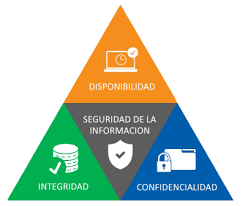
\includegraphics[width=6cm]{images/triada.png}
    \caption{Triada de la Información. Fuente: 4IT Networks \cite{triada}} 
    \label{fig:triada}
\end{figure}


\begin{itemize}
\item \textbf{Confidencialidad}: Es la propiedad que se refiere a que la información no esté disponible ni sea revelada a individuos, entidades o procesos no autorizados, Esta se debe definir de acuerdo con las características de los activos que se manejan en la empresa.
\item \textbf{Integridad}: Se refiere a la exactitud y completitud de la información. Esta propiedad es la que permite que la información sea precisa, coherente y completa desde su creación hasta su destrucción. 
\item \textbf{Disponibilidad}: Es la propiedad de la información que se refiere a que ésta debe ser accesible y utilizable por solicitud de una persona entidad o proceso autorizado cuando así lo requiera éste, en el momento y en la forma que se requiere ahora y en el futuro, al igual que los recursos necesarios para su uso.
\end{itemize}
\par\vspace{0.5cm}

A continuación, se presenta una tabla comparativa que resume los objetivos principales de estas normativas y estándares, así como los grupos a los que afectan:

\begin{table}[H]
\centering
\begin{tabular}{|m{2.5cm}|p{7.5cm}|p{5.5cm}|}
\hline
\textbf{Normativa / Estándar} & \textbf{Objetivo Principal} & \textbf{Afectan a} \\ \hline

ENS &
\begin{minipage}[c]{\linewidth}
\begin{itemize}
        \par\vspace{0.1cm}

  \item Establecer requisitos mínimos de seguridad.
  \item Proteger la información digital pública.
  \item Promover un enfoque basado en riesgos.    \par\vspace{0.1cm}

\end{itemize}
\end{minipage} &
\begin{minipage}[c]{\linewidth}
\begin{itemize}
  \item Organismos públicos.    \par\vspace{0.1cm}

  \item Empresas proveedoras del sector público.    \par\vspace{0.1cm}

\end{itemize}
\end{minipage} \\ \hline

LOPD-GDD &
\begin{minipage}[c]{\linewidth}
\begin{itemize}
    \par\vspace{0.1cm}
  \item Garantizar los derechos digitales.   

  \item Proteger datos personales.
  \item Adaptar el RGPD al ordenamiento español.    \par\vspace{0.1cm}

  \par\vspace{0.1cm}
\end{itemize}
\end{minipage} &
\begin{minipage}[c]{\linewidth}
\begin{itemize}
  \item Empresas y entidades que traten datos personales en España.  

\end{itemize}
\end{minipage} \\ \hline

RGPD (UE) &
\begin{minipage}[c]{\linewidth}
\begin{itemize} \par\vspace{0.1cm}
  \item Unificar normas de protección de datos en la UE.   

  \item Asegurar el control de los ciudadanos sobre sus datos.
  \item Establecer principios como la responsabilidad proactiva.    \par\vspace{0.1cm}

\end{itemize}
\end{minipage} &
\begin{minipage}[c]{\linewidth}
\begin{itemize}
  \item Cualquier organización que trate datos de ciudadanos europeos.    

\end{itemize}
\end{minipage} \\ \hline

Directiva NIS2 &
\begin{minipage}[c]{\linewidth}
\begin{itemize} \par\vspace{0.1cm}
  \item Aumentar la resiliencia cibernética.    

  \item Proteger sectores críticos.
  \item Establecer obligaciones de notificación de incidentes.    \par\vspace{0.1cm}

\end{itemize}
\end{minipage} &
\begin{minipage}[c]{\linewidth}
\begin{itemize}
  \item Empresas en sectores esenciales (energía, transporte, salud, servicios digitales, etc).
\end{itemize}
\end{minipage} \\ \hline

ISO/IEC 27001:2022 &
\begin{minipage}[c]{\linewidth}
\begin{itemize} \par\vspace{0.1cm}
  \item Implementar un SGSI efectivo.    
  \item Proteger la confidencialidad, integridad y disponibilidad de la información.
  \item Gestionar riesgos de forma continua.    \par\vspace{0.1cm}

\end{itemize}
\end{minipage} &
\begin{minipage}[c]{\linewidth}
\begin{itemize}
  \item Organizaciones que buscan certificación en gestión de seguridad.
\end{itemize}
\end{minipage} \\ \hline

\end{tabular}
\caption{Comparativa de normativas y estándares en ciberseguridad.}
\label{tabla:normativas}
\end{table}





\par\vspace{0.5cm}


\subsubsection{Metodologías de Auditoría en Ciberseguridad}
\par\vspace{0.5cm}

Para ejecutar auditorías completas y rigurosas en ciberseguridad, existen metodologías reconocidas a nivel global que garantizan un marco estructurado. Algunas de las más relevantes son:
\par\vspace{0.5cm}

\textbf{OWASP (Open Web Application Security Project):} Proporciona directrices y metodologías específicas enfocadas en la identificación y mitigación de vulnerabilidades en aplicaciones web, siendo clave para desarrolladores y auditores en la protección contra ataques comunes \cite{owasp}.
\par\vspace{0.5cm}

\textbf{OSSTMM (Open Source Security Testing Methodology Manual):} Metodología abierta que ofrece procedimientos exhaustivos para realizar pruebas de seguridad técnica, enfocada en un análisis objetivo, cuantitativo y ético de vulnerabilidades técnicas y operativas \cite{osstmm}.
\par\vspace{0.5cm}

\textbf{TIBER-EU (Threat Intelligence-Based Ethical Red Teaming):} Marco metodológico europeo para pruebas controladas de simulación de ataques informáticos complejos, utilizando inteligencia de amenazas reales para evaluar la resiliencia de entidades críticas frente a ataques avanzados \cite{tibereu}.
\par\vspace{0.5cm}

\textbf{NIST SP 800-53:} Publicación que ofrece un conjunto exhaustivo de controles recomendados por el NIST para mejorar la seguridad y privacidad de sistemas informáticos en organizaciones federales y comerciales, cubriendo aspectos desde la gestión del riesgo hasta controles técnicos y operacionales detallados \cite{nist80053}.
\par\vspace{0.5cm}

\textbf{NIST SP 800-115:} Guía técnica específica sobre cómo realizar pruebas de seguridad (pentesting) en redes y sistemas, estableciendo procedimientos detallados para planificación, ejecución y evaluación de resultados, siendo ampliamente usada para pruebas de seguridad profundas y efectivas \cite{nist800115}.
\par\vspace{0.5cm}


\subsection{Herramientas de pentesting}
\par\vspace{0.5cm}

La selección de herramientas de pentesting desempeña un papel fundamental en la eficacia de las auditorías de seguridad. Identificar las herramientas adecuadas permite detectar vulnerabilidades de forma precisa y eficiente, adaptándose a distintos escenarios 
como redes, aplicaciones web, servicios en la nube o incluso factores humanos a través de técnicas de ingeniería social. A partir de un análisis conjunto de diversas fuentes especializadas, se recopilaron las diez herramientas 
más utilizadas y valoradas en el ámbito del pentesting. \cite{felipe2024}

\begin{table}[H]
\caption{Herramientas de pentesting más empleadas}
\centering
\begin{tabular}{|m{5cm}|m{3.5cm}|m{8cm}|}
    \hline
    \textbf{Herramienta} & \textbf{Aplicación} & \textbf{Descripción} \\
    \hline
    
\includegraphics[width=0.7cm]{images/nmap.jpeg} \textbf{Nmap} & Test de penetración de redes & Escáner de redes y auditor de seguridad que permite descubrir hosts, servicios y vulnerabilidades activas. \\
    \hline
    
\includegraphics[width=0.6cm]{images/metasploit.jpeg} \textbf{Metasploit} & Desarrollo y ejecución de exploits & Framework completo para desarrollar, probar y ejecutar exploits en entornos controlados. \\
    \hline
    
\includegraphics[width=0.7cm]{images/burp.jpeg} \textbf{Burp Suite} & Auditoría de seguridad en aplicaciones web & Plataforma integrada para análisis de seguridad en aplicaciones web, capaz de interceptar, modificar y automatizar pruebas. \\
    \hline
    
\includegraphics[width=0.85cm]{images/kali.jpeg} \textbf{Kali Linux / Parrot OS} & Entornos completos para pentesting & Sistemas operativos especializados para pentesting que incluyen múltiples herramientas de auditoría, análisis forense e ingeniería inversa. \\
    \hline
    
\includegraphics[width=0.95cm]{images/nessus.png} \textbf{Nessus} & Escaneo de vulnerabilidades de red & Escáner que identifica configuraciones erróneas, parches faltantes y debilidades comunes en sistemas y redes. \\
    \hline
    
\includegraphics[width=0.7cm]{images/john.png} \textbf{John the Ripper} & Craqueo de contraseñas & Herramienta para descifrar contraseñas y evaluar su fortaleza en diferentes sistemas. \\
    \hline
    
\includegraphics[width=0.75cm]{images/wireshark.png} \textbf{Wireshark} & Análisis de tráfico de red & Analizador de protocolos que captura y examina en tiempo real el tráfico que circula por una red. \\
    \hline
    
\includegraphics[width=0.6cm]{images/zap.jpeg} \textbf{ZAP (Zed Attack Proxy)} & Escaneo de seguridad en aplicaciones web & Escáner enfocado en detectar vulnerabilidades durante el desarrollo de aplicaciones web. \\
    \hline
    \textbf{SQLmap} & Detección y explotación de inyecciones SQL & Automatiza la identificación y explotación de vulnerabilidades de inyección SQL en aplicaciones web. \\
    \hline
    
\includegraphics[width=0.6cm]{images/aircrack.jpeg} \textbf{Aircrack-ng} & Auditoría de redes Wi-Fi & Conjunto de herramientas para romper claves WEP y WPA/WPA2 y auditar la seguridad de redes inalámbricas. \\
    \hline
\end{tabular}
\begin{flushleft}\centering
    \footnotesize \textbf{Fuente:} Criterios de selección de herramientas para pentesting. \cite{felipe2024}
\end{flushleft}
\end{table}
\par\vspace{0.5cm}
Estas herramientas, junto con sus respectivas páginas oficiales para descarga o consulta, pueden encontrarse en el \hyperref[anexo:2]{\textbf{Anexo 2}}.

\par\vspace{0.5cm}


\subsection{Certificaciones del sector}
\par\vspace{0.5cm}

Por último, para aquellas personas interesadas en iniciarse en el campo de la ciberseguridad ofensiva, 
es fundamental contar con una guía clara que oriente su aprendizaje y desarrollo profesional. Las certificaciones 
profesionales cumplen un papel importante en este sentido, ya que no solo validan los conocimientos técnicos y las habilidades de la persona, sino que también proporcionan una formación progresiva para adquirir competencias en distintas áreas de la ciberseguridad. La selección de estas certificaciones ha sido elaborada a partir de fuentes formales y del conocimiento compartido en comunidades especializadas de hacking ético y pentesting, incluyendo foros, redes profesionales y grupos de intercambio de experiencias. Se incluyen algunas de las certificaciones más relevantes, ordenadas por nivel de dificultad dentro del área ofensiva, incluyendo una certificación fundamental en administración de sistemas Linux, que sirve de base para el dominio de entornos seguros.



\begin{itemize}
    \item \textbf{LPIC-1/2 (Linux Professional Institute Certification)}: Es la certificación de nivel básico/intermedio para administradores de sistemas Linux. Valida competencias en instalación, configuración, mantenimiento y administración de sistemas basados en Linux, incluyendo tareas de red y scripting en bash. Resulta especialmente útil como base sólida para profesionales que quieran profundizar en seguridad ofensiva y defensiva en entornos Unix.

    \item \textbf{eJPTv2 (eLearnSecurity Junior Penetration Tester)}: Ideal para principiantes en el campo del pentesting. Evalúa conocimientos básicos sobre redes, sistemas operativos, metodologías de pruebas de penetración y explotación de vulnerabilidades comunes. El examen es práctico y se realiza en un entorno de laboratorio simulado.

    \item \textbf{eWPT (eLearnSecurity Web Penetration Tester)}: Certificación especializada en seguridad de aplicaciones web.

    \item \textbf{eCPPTv2 (eLearnSecurity Certified Professional Penetration Tester)}: De nivel intermedio, esta certificación evalúa habilidades prácticas en pentesting interno y externo, incluyendo explotación de vulnerabilidades, escalada de privilegios, evasión de antivirus y generación de informes.

    \item \textbf{PNPT (Practical Network Penetration Tester)}: Emitida por TCM Security, esta certificación simula una auditoría real de red empresarial. El candidato debe realizar tareas de reconocimiento, explotación, post-explotación, pivoting y red teaming básico, y entregar un informe técnico al estilo profesional.

    \item \textbf{OSCP (Offensive Security Certified Professional)}: Considerada una de las certificaciones más exigentes y prestigiosas en pentesting. Exige comprometer múltiples máquinas en un entorno controlado durante un examen de 24 horas. Requiere dominio de técnicas como buffer overflows, escalada de privilegios, evasión de defensas, explotación manual y redacción exhaustiva de informes. Es un estándar de referencia en la industria de seguridad ofensiva.
\end{itemize}

\par\vspace{0.5cm}




\clearpage

\thispagestyle{nohead}




% -----------------------------------------------NIST SP 800-115-------------------------------------------------------------


\section{Metodología elegida: NIST SP 800-115}

\par\vspace{0.5cm}

Para la propuesta metodológica planteada en este trabajo, se toma como base fundamental la metodología NIST SP 800-115 debido a su amplia aceptación y versatilidad en auditorías técnicas de seguridad informática. Esta metodología se selecciona específicamente por su capacidad para adaptarse eficazmente a los objetivos establecidos por la empresa BeeHacker, sobre los cuales se sustenta nuestra propuesta de auditoría. 
\par\vspace{0.5cm}


El documento original consta de 80 páginas, divididas en cuatro fases fundamentales: planificación, descubrimiento, ataque y reporte. Estas fases aseguran una cobertura completa desde la definición del alcance hasta la generación de informes y recomendaciones finales. \cite{nist800115} 


\begin{figure}[H]
    \centering
    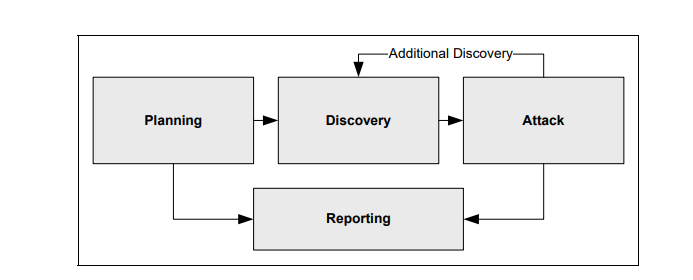
\includegraphics[width=13cm]{images/nist_800115.png}
    \caption{Metodología NIST SP 800-115. Fuente: \cite{nist800115}}
    \label{fig:nist_800115}
\end{figure}

A continuación, se presenta un desglose adaptado y resumido del contenido de la metodología NIST SP 800-115:


\subsection{Fase de Planificación (Planning Phase)}

Esta fase inicial implica la definición clara de los objetivos, el alcance y las restricciones de la auditoría. Se identifican los sistemas y activos a evaluar, se asignan responsabilidades, se establecen las reglas de compromiso (Rules of Engagement), y se gestiona la aprobación por parte de los responsables de la organización. La planificación también contempla la recopilación de información preliminar sobre la infraestructura, políticas de seguridad y nivel de madurez de la organización.


\subsection{Fase de Descubrimiento (Discovery Phase)}

En esta etapa se lleva a cabo la recolección de datos sobre los sistemas objetivo mediante técnicas pasivas y activas. 
Las técnicas pasivas incluyen el análisis de información disponible públicamente (OSINT), mientras que las técnicas activas abarcan escaneos de red, detección de puertos abiertos, 
identificación de servicios y sistemas operativos, así como la enumeración de posibles vulnerabilidades. El propósito es obtener una visión detallada del entorno evaluado sin interferir en su funcionamiento.

\par\vspace{0.5cm}
Una vez recopilada toda la información, se procede al análisis detallado de los descubrimientos con el objetivo de evaluar el nivel de riesgo asociado a cada vulnerabilidad identificada. Esta evaluación permite priorizar los posibles vectores de ataque y trazar un plan de acción estratégico para la siguiente fase.

\subsection{Fase de Ataque (Attack Phase)}

Esta fase simula un escenario real de intrusión con el fin de explotar las vulnerabilidades detectadas previamente. Las pruebas pueden incluir ataques de penetración, escalamiento de privilegios, evasión de controles de seguridad y acceso no autorizado a recursos. Aunque esta fase puede resultar intrusiva, es crucial para evaluar la efectividad de los mecanismos de defensa implementados. Siempre se ejecuta bajo estrictos parámetros éticos y de autorización.


\subsection{Fase de Reporte (Reporting Phase)}

Finalmente, se documentan los hallazgos obtenidos durante la auditoría. El informe debe ser claro, técnico y ejecutivo, incluyendo descripciones detalladas de las vulnerabilidades encontradas, evidencias de explotación (cuando corresponda), análisis de riesgos y recomendaciones específicas para mitigar o corregir las debilidades identificadas. Este reporte sirve como base para la toma de decisiones estratégicas de seguridad por parte de la organización.






















\clearpage
\thispagestyle{nohead}


% -----------------------------------------------MODELO------------------------------------------------------------

\section{Modelo de auditoría}
\par\vspace{0.5cm}


El presente capítulo tiene como finalidad exponer un modelo de auditoría de ciberseguridad que integra y sintetiza las fases, técnicas y prácticas empleadas por organizaciones especializadas en ciberseguridad, adaptándolas a la metodología base definida en el capítulo anterior. Este modelo ha sido desarrollado en colaboración con la empresa \textbf{BeeHacker}.
\par\vspace{0.5cm}

\textbf{BeeHacker} es una empresa de ciberseguridad ubicada en Mairena del Aljarafe (Sevilla), especializada en ofrecer servicios relacionados con el cumplimiento normativo, la ciberdefensa y las pruebas de penetración. Disponen de un equipo especializado en \textit{Blue Team} y \textit{SOC} (Security Operations Center), así como expertos en \textit{Pentesting}, responsables de la realización de auditorías de seguridad, ejercicios Red Team y análisis forense, incluyendo la respuesta ante incidentes de seguridad. \cite{beehacker}

\subsection*{Áreas de especialización de BeeHacker}

\begin{itemize}
    \item \textbf{OWASP}: Pruebas centradas en vulnerabilidades comunes del desarrollo web.
    \item \textbf{Seguridad legal / SGSI / ENS}: Adecuación a normativas y estándares como el ENS (Esquema Nacional de Seguridad) o sistemas de gestión de seguridad de la información.
    \item \textbf{Seguridad industrial}: Protección de entornos OT (tecnología operativa) e infraestructuras críticas.
\end{itemize}

Cabe destacar y agradecer especialmente la implicación del equipo de BeeHacker durante el desarrollo de este trabajo. Su disponibilidad para realizar entrevistas, reuniones y sesiones de formación ha sido clave tanto para el enfoque técnico del proyecto como para mi crecimiento personal. Han contribuido activamente a contextualizar el estado actual del sector de la ciberseguridad y a ofrecer una visión clara sobre sus desafíos y buenas prácticas.
\par\vspace{0.5cm}

El modelo que se presenta a continuación ha sido elaborado de forma iterativa a lo largo de dichas sesiones, resolviendo dudas y contrastando enfoques, con el objetivo de reflejar y poner en valor el trabajo que realiza BeeHacker en el marco de una auditoría de ciberseguridad orientada a PYMEs.


\par\vspace{0.5cm}

\subsection{Diseño propuesto por BeeHacker}
\par\vspace{0.5cm}

El modelo de auditoría propuesto se basa en un enfoque estructurado por capas, abarcando todos los vectores de ataque 
potenciales desde el perímetro exterior hasta los datos almacenados internamente. 
Este diseño tiene como objetivo principal proporcionar un listado de actividades que permita
auditar la ciberseguridad en una Pyme sin necesidad de poseer conocimientos técnicos avanzados. 



\par\vspace{0.5cm}

El modelo se compone específicamente de siete grandes bloques que permiten un análisis completo de la seguridad:

\begin{figure}[H]
    \centering
    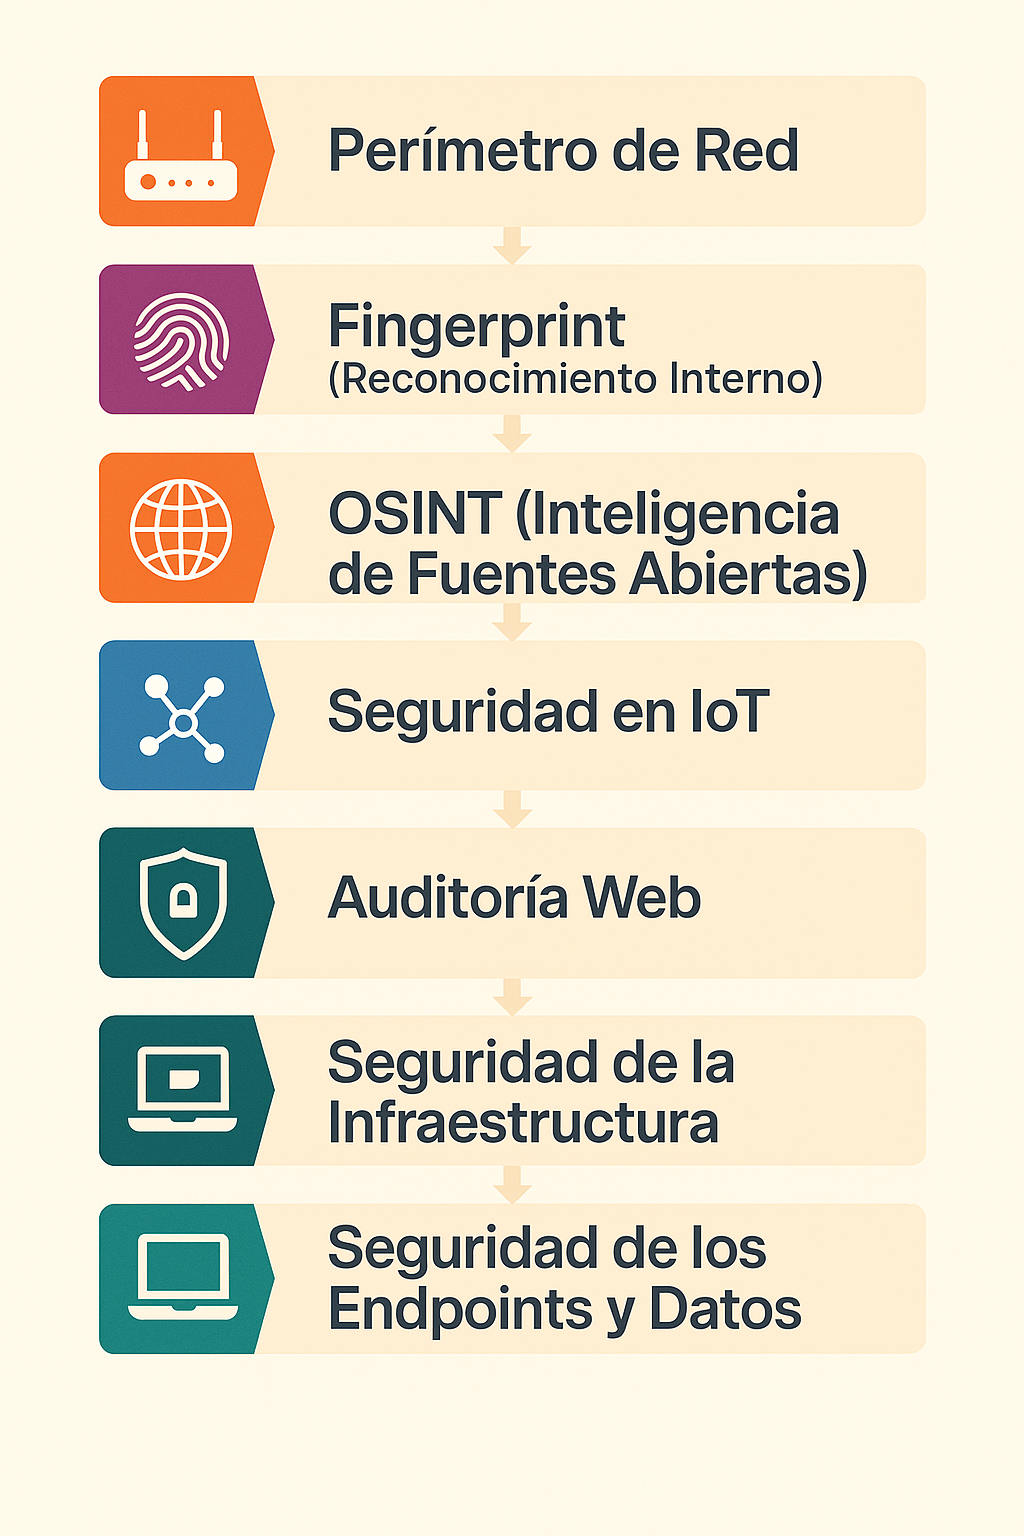
\includegraphics[width=0.45\textwidth]{images/diseno.png}
    \caption{Diagrama de flujo de los bloques del diseño del modelo de auditoría. Fuente: Elaboración propia}
    \label{fig:diseno_modelo_auditoria}
\end{figure}
\par\vspace{0.5cm}

\begin{enumerate}
    \item \textbf{Perímetro de Red:} Se analiza la exposición externa de la infraestructura desde la perspectiva de un atacante sin conocimiento previo. Se evalúan routers con configuraciones por defecto (telnet, SSH abiertos), firewalls mal configurados, accesos remotos sin cifrado, y redes inalámbricas vulnerables. Se incluyen pruebas sobre sistemas RADIUS, bypass de portales cautivos, detección de APs maliciosos (Rogue AP / Karma WiFi), análisis de seguridad inalámbrica y cifrado.

\item \textbf{Fingerprint (Reconocimiento Interno):} Se realiza un reconocimiento de red interno: análisis de la topología de red, detección activos en la red, enumeración de puertos abiertos y servicios activos en cada activo. 
El mapeo de red se complementa con un análisis de vulnerabilidades.

\item \textbf{OSINT (Inteligencia de Fuentes Abiertas):} Se recopila y analiza información pública sobre la organización para descubrir posibles vectores de ataque. Se utilizan motores como Google (GHDB), Shodan, Censys y Maltego para identificar servidores expuestos, credenciales filtradas, tecnologías empleadas y datos personales. Además, se evalúan técnicas de ingeniería social como phishing.

\item \textbf{Seguridad en IoT:} Dado que muchas pymes incorporan dispositivos inteligentes como cámaras, sensores, esta fase analiza posibles accesos no autorizados a través de estos dispositivos, los cuales suelen estar poco protegidos. Se revisa su firmware, autenticación, cifrado y su exposición en la red.
\item \textbf{Auditoría Web:} Se realizan pruebas de seguridad siguiendo las recomendaciones de OWASP. 

\item \textbf{Seguridad de Infraestructura:} Se revisa la arquitectura interna de la empresa: servidores, redes privadas, Active Directory, firewalls internos, y sistemas IDS/IPS. Se ejecutan pruebas de escalada de privilegios, pivoting, análisis de red, y se evalúa la configuración segura de cada elemento. También se estudian los logs y mecanismos de monitoreo, identificando posibles brechas de seguridad.

\item \textbf{Seguridad de Endpoints y Datos:} Se analiza la protección de los dispositivos finales utilizados por los empleados, donde suele recaer una parte crítica de la seguridad. Se auditan políticas de contraseñas, cifrado de disco, control de dispositivos USB, protección frente a malware, uso de software legítimo, backup de información, y sistemas de almacenamiento.

\end{enumerate}

\par\vspace{0.5cm}




A continuación, se detallan los objetivos y actividades que componen este diseño:

\par\vspace{0.5cm}


\subsubsection{Análisis del Perímetro de Red}

Con el análisis del perímetro de red, intentamos identificar los puntos débiles de la infraestructura desde la perspectiva de un atacante externo, sin conocimiento de la arquitectura interna.

\begin{table}[H]
    \centering
    \renewcommand{\arraystretch}{1.4}
    \begin{tabular}{|p{1.4cm}|p{3.9cm}|p{5.3cm}|p{4.2cm}|}
    \hline
    \textbf{ID} & \textbf{Objetivo} & \textbf{Actividades} & \textbf{Herramientas}\\
    \hline
    OBJ-01 & Detectar redes inalámbricas disponibles & Enumeración de SSIDs visibles y ocultos & Airodump-ng, Wireshark\\
    \hline
    OBJ-02 & Evaluar seguridad de cifrado WiFi & Identificar tipo de cifrado (WEP/WPA/WPA2/Enterprise) captura de handshake & Airodump-ng, hcxdumptool, Aircrack-ng \\
    \hline
    OBJ-03 & Realizar ataques de fuerza bruta a redes inseguras & Diccionario sobre handshake capturado & Aircrack-ng, hashcat \\
    \hline
    OBJ-04 & Validar seguridad de portal cautivo & Intento de bypass (DNS spoof, phishing, MitM) & Bettercap, mitmproxy, macchanger\\
    \hline
    OBJ-05 & Simular Rogue AP y ataques Karma & Clonado de SSID, AP falso para interceptar clientes & WiFi Pineapple, Hostapd, EvilTrust \\
    \hline
    OBJ-06 & Detectar APs mal configurados o sospechosos & Escaneo de redes abiertas, SSID duplicados, canales raros & Airodump-ng, Wireshark\\
    \hline
    OBJ-07 & Identificar routers con credenciales por defecto & Prueba de acceso a SSH, Telnet, interfaces web & Nmap, Hydra \\
    \hline
    \end{tabular}
    \caption{Tabla de objetivos en el análisis del perímetro de red}
    \end{table}
    
\par\vspace{0.5cm}






\subsubsection{Fingerprint (Reconocimiento Interno)}

Una vez dentro de la red, se analizan los diferentes dispositivos conectados y sus diferentes vulnerabilidades, para trazar un plan de ataque.

\begin{table}[H]
\centering
\renewcommand{\arraystretch}{1.4}
    \begin{tabular}{|p{1.4cm}|p{3.9cm}|p{5.3cm}|p{4.2cm}|}
\hline
\textbf{ID} & \textbf{Objetivo} & \textbf{Actividades} & \textbf{Herramientas}  \\
\hline
OBJ-08 & Mapeo de la red interna & Descubrimiento de dispositivos, gateways, rutas, subredes & Nmap, Neptus  \\
\hline
OBJ-09 & Análisis de puertos abiertos & Escaneo de red interna, detección de servicios accesibles & Nmap, Masscan, Neptus  \\
\hline
OBJ-10 & Identificación de servicios y versiones & Fingerprinting de servicios, banner grabbing, OS detection & Nmap, WhatWeb, Netcat  \\
\hline
OBJ-11 & Detección de vulnerabilidades conocidas & Escaneo de CVEs, servicios sin parches, versiones antiguas & Nessus, Exploit-db, WhatWeb  \\
\hline

\end{tabular}
\caption{Tabla de objetivos en la fase de Fingerprint interno}
\end{table}


\par\vspace{0.5cm}



\subsubsection{OSINT e Ingeniería Social}

Esta fase se centra en la obtención de información utilizando fuentes abiertas (Open Source Intelligence), recopilando datos públicos que puedan ser útiles para identificar vectores de ataque antes de cualquier interacción directa con los sistemas. Se complementa con técnicas de ingeniería social para evaluar el factor humano.

\begin{table}[H]
\centering
\renewcommand{\arraystretch}{1.4}
    \begin{tabular}{|p{1.4cm}|p{3.9cm}|p{5.3cm}|p{4.2cm}|}
\hline
\textbf{ID} & \textbf{Objetivo} & \textbf{Actividades} & \textbf{Herramientas}  \\
\hline
OBJ-12 & Recolectar información de buscadores genéricos & Búsquedas avanzadas con dorks, índice de documentos, paneles expuestos & Google, Google Hacking DB (GHDB)  \\
\hline
OBJ-13 & Identificar activos expuestos & Recolección de IPs públicas, puertos y servicios accesibles & Shodan, Censys  \\
\hline
OBJ-14 & Analizar relaciones y metadatos en redes y dominios & Investigación de nombres, emails, metadatos de documentos y relaciones entre entidades & Maltego, theHarvester \\
\hline
OBJ-15 & Buscar credenciales filtradas y contraseñas públicas & Consultas sobre leaks, validación de emails y dominios comprometidos & DeHashed, HaveIBeenPwned  \\
\hline
OBJ-16 & Evaluar la respuesta humana frente a ataques simulados & Pruebas de phishing, manipulación, evaluación de políticas internas  & GoPhish, RubberDucky \\
\hline
\end{tabular}
\caption{Tabla de objetivos en la fase OSINT e Ingeniería Social}
\end{table}



\par\vspace{0.5cm}




\subsubsection{Seguridad en IoT}

Los dispositivos IoT suelen carecer de medidas de seguridad sólidas y se convierten en vectores frecuentes de ataque. Esta fase se enfoca en el análisis del tráfico de red, servicios inseguros, firmware, y protocolos específicos utilizados por dispositivos conectados.

\begin{table}[H]
\centering
\renewcommand{\arraystretch}{1.4}
    \begin{tabular}{|p{1.4cm}|p{3.9cm}|p{5.3cm}|p{4.2cm}|}
\hline
\textbf{ID} & \textbf{Objetivo} & \textbf{Actividades} & \textbf{Herramientas}  \\
\hline
OBJ-17 & Identificar dispositivos IoT en la red & Escaneo de red, fingerprinting de fabricantes, búsqueda de dispositivos por MAC y puertos comunes & Nmap, Wireshark  \\
\hline
OBJ-18 & Analizar protocolos IoT y tráfico de red & Captura y análisis de paquetes en protocolos propietarios (MQTT, CoAP, BLE, UPnP) & Wireshark  \\
\hline
OBJ-19 & Evaluar la seguridad de interfaces y APIs & Inspección de endpoints HTTP, comandos remotos, autenticación débil o inexistente & Postman, Burp Suite  \\
\hline
OBJ-20 & Detectar firmware inseguro o mal configurado & Extracción y análisis de firmware, validación de backdoors y servicios inseguros & Wireshark  \\
\hline
OBJ-21 & Atacar dispositivos vulnerables & Explotación de servicios abiertos, contraseñas por defecto, ejecución remota de comandos & Metasploit, hydra, scripts personalizados  \\
\hline
\end{tabular}
\caption{Tabla de objetivos en la auditoría de dispositivos IoT}
\end{table}

\par\vspace{0.5cm}


\subsubsection{Auditoría Web}

En esta fase se analiza por completo la plataforma web, partiendo desde el propio servidor donde se aloja. Se siguen los pasos establecidos por la metodología OWASP para detectar las vulnerabilidades más críticas.

\begin{table}[H]
\centering
\renewcommand{\arraystretch}{1.4}
\begin{tabular}{|p{1.4cm}|p{4cm}|p{4.8cm}|p{3.8cm}|p{2.5cm}|}
\hline
\textbf{ID} & \textbf{Objetivo} & \textbf{Actividades} & \textbf{Herramientas}  \\
\hline
OBJ-22 & Analizar el servidor web y servicios asociados & Fingerprinting, detección de versiones, servicios activos, configuración & WhatWeb, Nikto, Nmap scripts  \\
\hline
OBJ-23 & Identificar servicios vulnerables o expuestos & Enumeración de directorios, endpoints, tecnologías utilizadas & Dirb, Gobuster, Wappalyzer  \\
\hline
OBJ-24 & Detectar vulnerabilidades OWASP & SQLi, XSS, IDOR, RCE, SSRF, CSRF, XXE, etc. & Burp Suite, gestores de contenido \\
\hline
OBJ-25 & Validar mecanismos de autenticación & Fuerza bruta, evasión de login, análisis de formularios & Hydra, Burp Intruder, wfuzz, GoBuster  \\
\hline
OBJ-26 & Evaluar la gestión de sesiones & Análisis de cookies, tokens, regeneración y caducidad de sesiones &  Burp Suite  \\
\hline
OBJ-27 & Probar mecanismos de autorización & Escalada de privilegios, acceso a funciones restringidas & Burp Suite, Postman \\
\hline
OBJ-28 & Validar controles de entrada/salida & Pruebas de validación del lado cliente y servidor, bypasses comunes & Burpsuite, payloads manuales  \\
\hline
OBJ-29 & Explorar la aplicación (crawling/spidering) & Recolección automatizada de rutas y formularios & Burpsuite \\
\hline
OBJ-30 & Realizar fuerza bruta y fuzzing sobre parámetros & Testeo de inputs, formularios & wfuzz, Burpsuite, sqlmap  \\
\hline
OBJ-31 & Evaluar la criptografía usada en la aplicación & Análisis de algoritmos de hash, cifrados, tokens y secretos & Burp Crypto  \\
\hline
\end{tabular}
\caption{Tabla de objetivos en la auditoría de aplicaciones web}
\end{table}

\par\vspace{0.5cm}




\subsubsection{Seguridad de la Infraestructura}

Esta fase abarca pruebas sobre el núcleo central de la seguridad en la organización.

\begin{table}[H]
\centering
\renewcommand{\arraystretch}{1.4}
\begin{tabular}{|p{1.4cm}|p{4.2cm}|p{4.8cm}|p{3.8cm}|p{2.3cm}|}
\hline
\textbf{ID} & \textbf{Objetivo} & \textbf{Actividades} & \textbf{Herramientas}  \\
\hline
OBJ-32 & Evaluar configuración del firewall & Identificación de puertos permitidos, pruebas de evasión, reglas de filtrado & Nmap, Scapy, tcptraceroute  \\
\hline
OBJ-33 & Verificar funcionamiento de IDS/IPS & Generación de tráfico sospechoso, análisis de alertas y detección de ataques & Metasploit, Nmap  \\
\hline
OBJ-34 & Analizar seguridad del servidor interno & Revisión de servicios, versiones, credenciales por defecto y vulnerabilidades conocidas & Nmap, Nikto, Nessus  \\
\hline
OBJ-35 & Realizar pruebas sobre Active Directory & Enumeración de usuarios, grupos, GPOs, tickets Kerberos & NetExec, CrackMapExec, Kerbrute, impacket  \\
\hline
OBJ-36 & Analizar tráfico y segmentación de red & Sniffing, detección de redes planas, protocolos en claro, ARP poisoning & Bettercap, Responder, Wireshark, tcpdump  \\
\hline
OBJ-37 & Realizar escalada de privilegios en el entorno & Búsqueda de binarios SUID, permisos mal configurados, exploits locales & GTFOBins, ExploitDB  \\
\hline
OBJ-38 & Ejecutar técnicas de pivoting y movimiento lateral & Conexión a otras redes o máquinas a través de un host comprometido & Chisel, ProxyChains, SSH tunneling, Metasploit  \\
\hline
\end{tabular}
\caption{Tabla de objetivos en la evaluación de la seguridad de la infraestructura}
\end{table}


\par\vspace{0.5cm}





\subsubsection{Seguridad de Endpoints y Datos}

Esta fase se enfoca en los dispositivos cliente de la organización, evaluando su configuración de seguridad, control de accesos, privilegios de usuario, y posibles vectores de evasión de controles mediante proxies, software no autorizado o escaladas locales.
Además, se evalúan un conjunto de test sobre el almacenamiento de los datos y su sistema de respaldo.

\begin{table}[H]
\centering
\renewcommand{\arraystretch}{1.4}
\begin{tabular}{|p{1.4cm}|p{4.2cm}|p{4.8cm}|p{3.8cm}|}
\hline
\textbf{ID} & \textbf{Objetivo} & \textbf{Actividades} & \textbf{Herramientas}  \\
\hline
OBJ-39 & Evaluar configuración de roles y perfiles de usuario & Verificación de restricciones según rol, acceso a configuraciones y consolas & Manual, PowerShell  \\
\hline
OBJ-40 & Verificar control de puertos USB y dispositivos externos & Comprobación de bloqueo, acceso a discos externos, ejecución automática & USB Rubber Ducky, scripts batch, manual  \\
\hline
OBJ-41 & Comprobar bypass de proxy corporativo & Intento de acceso directo a Internet, uso de túneles y software alternativo & proxychains, TOR, chisel, VPN port forwarding  \\
\hline
OBJ-42 & Instalar y ejecutar software no autorizado & Prueba con aplicaciones portables o autoejecutables desde usuarios limitados & TOR Browser, portable apps, reverse shells  \\
\hline
OBJ-43 & Verificar restricciones sobre terminales y consolas & Evaluar si un perfil básico puede lanzar CMD, PowerShell o intérpretes & Terminal  \\
\hline
OBJ-44 & Evaluar políticas y mecanismos de backup & Revisión de la frecuencia, almacenamiento, redundancia y pruebas de restauración de copias de seguridad & Documentación, entrevistas, herramientas de backup \\
\hline
OBJ-45 & Analizar almacenamiento y cifrado de datos & Identificar dónde y cómo se almacenan datos sensibles, qué bases de datos se usan y si los datos están cifrados en reposo y en tránsito & Auditoría documental, herramientas de análisis de cifrado \\
\hline
OBJ-46 & Evaluar políticas de privacidad y protección de datos sensibles & Revisión de políticas internas para manejo de datos sensibles, control de acceso y auditorías de cumplimiento & Entrevistas, revisión documental \\
\hline
OBJ-47 & Verificar uso de contraseñas robustas y controles de autenticación & Comprobación de políticas de longitud, complejidad, expiración y almacenamiento seguro de contraseñas & Auditoría técnica, herramientas de análisis de políticas \\
\hline
\end{tabular}
\caption{Tabla de objetivos en la auditoría de seguridad de endpoints y datos}
\end{table}
\par\vspace{0.5cm}




\clearpage

\thispagestyle{nohead}

















% -----------------------------------------------REQUISITOS------------------------------------------------------------

\section{Requisitos previos a la auditoría}
\par\vspace{0.5cm}
En esta sección se detallan los requisitos previos necesarios para realizar una auditoría de ciberseguridad, en virtud de la metodología seleccionada previamente, la \textbf{NIST SP 800-115}, y siguiendo las recomendaciones aportadas por el CTO de \textbf{BeeHacker}. 
\par\vspace{0.5cm}

A continuación, se recogen los requisitos previos comunes a todo proceso de auditoría, según los marcos analizados.

\par\vspace{0.5cm}

\begin{enumerate}
\item \textbf{Formalización previa}: Establecer por escrito los siguientes documentos:

\begin{itemize}
\item \textbf{Acuerdo de Confidencialidad (NDA)}: Define el compromiso de confidencialidad respecto a toda la información sensible, técnica u organizativa que sea compartida durante la auditoría. Su objetivo es garantizar que ningún dato se utilice con fines ajenos al proyecto ni se divulgue sin autorización.

\item \textbf{Acuerdo de Servicios}: Establece los objetivos concretos, el alcance detallado, la duración estimada y las condiciones generales de la colaboración. Sirve como base para planificar y organizar el trabajo de forma estructurada y transparente.

\item \textbf{Autorización para Pruebas Técnicas}: Permite expresamente la realización de actividades técnicas como análisis de red, detección de vulnerabilidades, pruebas de acceso o campañas controladas de ingeniería social. Además, delimita qué sistemas están autorizados y bajo qué condiciones deben desarrollarse las pruebas.
\end{itemize}

\item \textbf{Marco normativo y regulatorio}: Asegurar que la auditoría se alinea con las normativas vigentes aplicables, como el Esquema Nacional de Seguridad (ENS), el Reglamento General de Protección de Datos (RGPD), la ISO/IEC 27001 y otras normativas sectoriales o internas relevantes.

\item \textbf{Identificación detallada de activos}: Solicitar un inventario completo, actualizado y validado de los sistemas, redes, aplicaciones y dispositivos que serán objeto de análisis durante la auditoría.

\item \textbf{Análisis de riesgos y medidas preventivas}: Antes de ejecutar cualquier acción técnica, es fundamental realizar una evaluación de los riesgos asociados a las pruebas de seguridad. Este análisis considera el impacto potencial sobre la disponibilidad, integridad y confidencialidad de los sistemas auditados. Se identifican los servicios críticos y se diseñan estrategias de mitigación para evitar interrupciones no deseadas, como realizar pruebas en entornos controlados o fuera del horario operativo.

\item \textbf{Preparación técnica y metodológica}: En esta auditoría se empleará la metodología desarrollada en los próximos capítulos.

\item \textbf{Comunicación y coordinación}: Durante toda la auditoría se mantendrán abiertos canales de comunicación estructurados entre el equipo auditor y los responsables designados por la organización auditada. Se definirán personas de contacto técnico y organizativo, así como los medios de notificación para incidentes, entregas de resultados intermedios y coordinación de accesos. Esta coordinación incluye reuniones previas, revisiones de estado y una reunión de cierre. La documentación generada en cada fase se compartirá a través de repositorios seguros o canales cifrados previamente acordados.

\item \textbf{Planificación y cronograma}: La auditoría seguirá un calendario de trabajo estructurado en fases, con fechas estimadas de inicio y fin para cada bloque. Este cronograma permitirá a la organización auditada conocer con antelación las actividades previstas, asignar recursos y supervisar el cumplimiento de los objetivos. Las fases estarán alineadas con el modelo secuencial definido en el plan metodológico de auditoría.

\item \textbf{Definición y organización del equipo auditor}: La estructura del equipo auditor debe estar claramente definida desde el inicio del proyecto. Se especificarán los profesionales que integran el equipo, incluyendo sus perfiles técnicos, funciones asignadas y grado de responsabilidad dentro del proceso. Asimismo, se establecerán los flujos de comunicación internos y los canales oficiales de interlocución con la entidad auditada, garantizando una coordinación eficaz durante todas las fases de la auditoría.
\end{enumerate}














































\clearpage
\thispagestyle{nohead}


%------------------PROPUESTA-------------------------------------------------------
\section{Propuesta metodológica de auditoría}

\par\vspace{0.5cm}
Este capítulo constituye el núcleo central del presente trabajo. A partir de toda la información recopilada en secciones anteriores, y tomando como referencia las fases establecidas por la \textbf{NIST SP 800-115}, así como los objetivos definidos por la empresa \textbf{BeeHacker}, se ha desarrollado una propuesta metodológica propia para la realización de auditorías de ciberseguridad.

\par\vspace{0.5cm}
El objetivo de esta sección es sintetizar y estructurar de forma secuencial todos los conocimientos y buenas prácticas analizadas, creando así un modelo accesible, replicable y comprensible incluso para profesionales sin experiencia previa en auditorías de ciberseguridad. Esta metodología no solo sigue el enfoque de evaluación técnica de la NIST, sino que incorpora objetivos concretos, herramientas recomendadas (de las cuales se ilustran mediante ejemplos prácticos su aplicación sin entrar en detalle), criterios de decisión y buenas prácticas organizativas validadas por \textbf{Ramón}, CTO de la empresa colaboradora \textbf{BeeHacker}.

\par\vspace{0.5cm}
El resultado es una metodología estructurada por fases, pensada para ofrecer una visión global del proceso de auditoría de ciberseguridad desde una perspectiva práctica y completa. A continuación, se exponen en detalle las fases secuenciales que componen la propuesta.


\par\vspace{0.5cm}

\subsection{Fase de Planificación de la Auditoría}
\par\vspace{0.5cm}

La fase de planificación representa el punto de partida formal del proceso de auditoría. En esta etapa se establecen las bases necesarias para garantizar que el trabajo se desarrolle de forma estructurada, controlada y alineada con los objetivos del proyecto. Es aquí donde se consolidan todos los acuerdos documentales previos, como el Acuerdo de Confidencialidad (NDA), el Acuerdo de Servicios y la Autorización para Pruebas Técnicas, descritos previamente en los requisitos.
\par\vspace{0.5cm}

El propósito principal de esta fase es definir con precisión el alcance de la auditoría, delimitar los sistemas y procesos que serán objeto de análisis y establecer el marco operativo bajo el cual se ejecutarán las pruebas. Para ello, resulta esencial mantener una comunicación directa con el responsable de seguridad de la empresa.
\par\vspace{0.5cm}

Una entrevista estructurada con esta persona clave permitirá al auditor obtener una visión global del entorno a auditar. A través de esta conversación se abordarán los grandes bloques que guiarán el resto de la auditoría, enfocándose especialmente en:

\begin{itemize}
\item La solicitud de un inventario de activos actualizado, que incluya servidores, estaciones de trabajo, dispositivos de red y servicios relevantes.
\item La obtención de un esquema detallado de la topología de red, incluyendo segmentaciones, conexiones externas, y sistemas críticos.
\item El acceso a las políticas de seguridad vigentes, tanto técnicas como organizativas, que regulan el comportamiento del personal y la gestión de los sistemas, con el fin de analizarlas y comprobar su cumplimiento
efectivo durante el desarrollo de las fases técnicas de la auditoría
\item La revisión, si procede, de informes o resultados de auditorías previas que puedan aportar contexto o antecedentes sobre el entorno.
\item La evaluación inicial del nivel de seguridad mediante una batería de preguntas dirigidas a cada uno de los bloques propuestos. Esto permite contrastar las afirmaciones del personal entrevistado con las evidencias técnicas que se obtendrán posteriormente.
\end{itemize}

Toda esta información permitirá afinar el enfoque técnico, ajustar las herramientas a utilizar, establecer prioridades en el análisis de riesgos y adecuar la metodología al entorno específico.
\par\vspace{0.5cm}

Una vez realizado este análisis preliminar y formalizada la documentación legal y técnica, se considerará que existe un marco de trabajo completamente definido. A partir de este momento, el equipo auditor podrá organizarse internamente, verificar la disponibilidad de las herramientas necesarias, confirmar la composición del equipo de trabajo y establecer fecha para el inicio de la siguiente fase.
\par\vspace{0.5cm}


\subsection{Fase de Descubrimiento de la Auditoría}
\par\vspace{0.5cm}

En esta fase se lleva a cabo la recopilación de información técnica sobre los sistemas y redes que serán objeto de auditoría. El objetivo es obtener información relevante acerca de los activos, servicios y configuraciones existentes, así como identificar vulnerabilidades o puntos débiles potencialmente explotables por un atacante.


\subsubsection{Análisis Externo de Redes Inalámbricas}
\label{sec:analisis_redes_inalambricas}


\par\vspace{0.5cm}
Inicialmente, se realiza un reconocimiento pasivo de las redes inalámbricas disponibles, lo que permite detectar tanto redes visibles como ocultas en el área de alcance. Durante este análisis se busca recopilar datos esenciales como el SSID, canal, BSSID, tipo de cifrado y potencia de la señal. Asimismo, se pretende capturar, cuando sea posible, el handshake de la red, fundamental para realizar posteriormente ataques de fuerza bruta que evalúen la seguridad del cifrado implementado.

\par\vspace{0.5cm}
\subsubsection*{Herramientas}
\begin{itemize}
    \item \textbf{Airodump-ng}: Herramienta de captura de paquetes de datos de redes WiFi, que proporciona información detallada sobre las redes detectadas.
    \item  \textbf{Wireshark}: Herramienta de captura y análisis de tráfico de red, que permite examinar los paquetes en detalle.
    \item \textbf{Antena WiFi}: Adaptador inalámbrico compatible con modo monitor, preferiblemente que soporte tanto las frecuencias de 2,4 GHz como las de 5 GHz. Si además soporta modo AP, se pueden realizar ataques avanzados como "rogue AP".
\end{itemize}

\par\vspace{0.5cm}

\subsubsection*{Prueba de concepto}

Esta técnica utiliza \textbf{Airodump-ng} para capturar tráfico de redes WiFi y realizar ataques de fuerza bruta sobre los handshakes capturados. El procedimiento comienza configurando la antena en modo monitor, seguido del escaneo de redes inalámbricas disponibles para seleccionar la red objetivo. Se debe registrar el BSSID y el canal específico para proceder a capturar el handshake mediante técnicas de desautenticación, que desconectan momentáneamente a los clientes obligándolos a reconectarse y generando el handshake.
\par\vspace{0.5cm}

Este handshake posteriormente será explotado mediante fuerza bruta para evaluar la robustez de la contraseña.

\par\vspace{0.5cm}

\begin{lstlisting}[language=bash, style=terminalstyle, caption=Captura WPA2 con Aircrack-ng]
    # Configuración de la antena en modo monitor
$ sudo airmon-ng start wlan0
    # Escaneo de redes WiFi disponibles
$ sudo airodump-ng wlan0mon
    # Selección de la red objetivo y captura del handshake
$ sudo airodump-ng --bssid BSSID --channel CHANNEL -w capture wlan0mon
    # Desautenticación de clientes para capturar el handshake en paralelo con airodump-ng
$ sudo aireplay-ng -0 9 -a BSSID -c CLIENT_MAC wlan0mon
    # Análisis del handshake capturado
$ sudo aircrack-ng -w /path/to/wordlist.txt capture-01.cap
\end{lstlisting}



\subsubsection*{Resultados esperados}

Se espera obtener los siguientes resultados clave tras la ejecución de las herramientas de análisis de redes inalámbricas:

\begin{itemize}
    \item \textbf{Inventario detallado de redes detectadas} (visibles y ocultas), incluyendo información como el \textit{SSID}, canal, \textit{BSSID}, tipo de cifrado y potencia de señal.
    
    \item \textbf{Captura del handshake WPA/WPA2}, que servirá para evaluar posteriormente la robustez de la contraseña mediante técnicas de fuerza bruta o diccionario, y así estimar la complejidad real de explotación.
\end{itemize}

\vspace{1em}

\begin{table}[H]
\centering
\renewcommand{\arraystretch}{1.2}
\begin{tabular}{|l|c|l|c|c|}
\hline
\textbf{SSID} & \textbf{Canal} & \textbf{BSSID} & \textbf{Cifrado} & \textbf{Potencia (dBm)} \\
\hline
WLAN-Casa     & 6      & 00:14:22:01:23:45 & WPA2 & -45 \\
Red Oculta    & 11     & A1:B2:C3:D4:E5:F6 & WPA2 & -60 \\
Biblioteca    & 1      & 12:34:56:78:9A:BC & WEP      & -72 \\
INVITADOS     & 3      & DE:AD:BE:EF:00:01 & Abierta  & -50 \\
\hline
\end{tabular}
\caption{Ejemplo de redes inalámbricas detectadas con Airodump-ng}
\label{tab:redes_detectadas}
\end{table}
\subsubsection*{Limitaciones}

\begin{itemize}
    \item \textbf{Limitación de análisis externo:} Puede verse afectado por firewalls avanzados, WAFs, mecanismos de bloqueo o listas blancas que filtran escaneos sospechosos.
    
    \item \textbf{Redes ocultas:} La detección depende del tráfico activo de clientes conectados; sin actividad, estas redes podrían no detectarse.
    
    \item \textbf{Desautenticación inefectiva:} Esta técnica podría fallar si no hay clientes conectados o si no existe tráfico activo.
\end{itemize}

\par\vspace{0.5cm}
































\subsubsection{Análisis Interno de Redes (Fingerprint)}

Una vez se logra acceso a la red, el objetivo es realizar un reconocimiento interno exhaustivo para identificar dispositivos conectados, configuraciones, y vulnerabilidades potenciales. El propósito es mapear claramente la topología interna, descubrir dispositivos, puertos y servicios activos, y evaluar vulnerabilidades relacionadas.

\par\vspace{0.5cm}
\subsubsection*{Herramientas}
Se emplean herramientas especializadas como \textbf{Nmap} o \textbf{Masscan} para realizar escaneos detallados. Además, conviene usar 
herramientas automatizdas como \textbf{Nessus} para ofrecer una primera visión clasificada de vulnerabilidades según su severidad.

\par\vspace{0.5cm}
\subsubsection*{Prueba de concepto}
El proceso comienza con un primer barrido de red mediante \textbf{Nessus}, para lo cual es fundamental identificar previamente el entorno en el que nos encontramos. Esto implica reconocer la red local y determinar su bloque \textit{CIDR}, con el objetivo de conocer el rango de direcciones IP disponibles y asegurarnos de que el análisis abarque todos los dispositivos posibles, evitando dejar zonas sin explorar.
\par\vspace{0.5cm}

Una vez definido el rango de red, se configura el escaneo desde la interfaz de Nessus, seleccionando la opción \textbf{Advanced Scan}, que permite personalizar el reconocimiento inicial según las necesidades del entorno.
\par\vspace{0.5cm}

Paralelamente, puede ejecutarse un proceso de enumeración de hosts activos mediante herramientas como \textbf{Nmap} o \textbf{Masscan}, utilizando técnicas basadas en \textit{ICMP} o \textit{ARP}. Es importante conocer cómo funcionan estos comandos, ya que algunos dispositivos podrían estar protegidos por firewalls o configuraciones que impidan una detección directa. En estos casos, el uso de scripts personalizados puede ser clave para mejorar la visibilidad y completar el mapeo de red de forma más precisa.

\par\vspace{0.5cm}

\begin{lstlisting}[language=bash, style=terminalstyle, caption=Escaneo de activos en la red]
    # Escaneo de red ICMP para identificar hosts activos
$ sudo nmap -sn 192.168.0.0/24
   # Escaneo de red con Masscan para identificar hosts activos 
$ sudo masscan 192.168.0.0/24 -p0-65535 --rate=1000
\end{lstlisting}


Una vez hemos identificado todos los activos a nuestro alcance, procederemos a enumerarlos con Nmap para obtener información sobre los puertos que tienen abierto y el servicio que está ejecutando cada uno de ellos.

\begin{lstlisting}[language=bash, style=terminalstyle, caption=Escaneo de puertos y servicios con Nmap]
    # Escaneo de puertos con Nmap
$ sudo nmap -p- --open -sS --min-rate 5000 -vvv -n -Pn 192.168.0.2 -oG allPorts
    # Escaneo de servicios con Nmap a los puertos abiertos del host
$ sudo nmap -sCV -p22,80,443 192.168.0.2 -oX scanService.xml
    # Convertir el resultado a un formato legible html
$ xsltproc scanService.xml -o scanService.html
\end{lstlisting}



Los comandos mostrados anteriormente representan ejemplos básicos del uso de estas herramientas para la detección de activos y escaneo de puertos. Sin embargo, estas herramientas ofrecen una gran variedad de parámetros adicionales que permiten ajustar el comportamiento del análisis en función de los objetivos y restricciones del entorno.
\par\vspace{0.5cm}
Es posible configurar escaneos más \textbf{sigilosos} para evitar la detección por firewalls o sistemas de prevención de intrusiones (IPS), así como escaneos más \textbf{agresivos} y rápidos cuando no se requiere discreción.
\par\vspace{0.5cm}
Un desglose detallado de estas opciones avanzadas, se encuentra disponible en el \hyperref[anexo:4]{\textbf{Anexo 4}}.

\subsubsection*{Resultados esperados}
\begin{itemize}

    \item \textbf{Topología interna detallada:} Mapeo completo de dispositivos conectados, gateways y subredes detectadas. 
    
    \item \textbf{Inventario de servicios y puertos:} Listado exhaustivo por dispositivo de los puertos abiertos, servicios en ejecución y protocolos asociados.
\end{itemize}

\subsubsection*{Limitaciones}

\begin{itemize}
   
    \item \textbf{Mecanismos de seguridad:} Firewalls, sistemas IDS/IPS o configuraciones personalizadas pueden bloquear escaneos o generar falsos positivos/negativos.
    
    \item \textbf{Rendimiento en redes complejas:} En redes mal segmentadas o muy extensas, el proceso puede volverse lento o ineficiente sin optimización adecuada.
    
    \item \textbf{Técnicas de evasión:} En algunos casos, será imprescindible aplicar estrategias de escaneo más avanzadas para evitar ser detectado.
\end{itemize}

\par\vspace{0.5cm}

\subsubsection{Análisis Interno de Tráfico de Red}

Una vez identificada la topología de red y los dispositivos activos, se procede a realizar un análisis pasivo del tráfico con el objetivo 
de obtener información sobre los protocolos en uso, detectar servicios inseguros, descubrir dispositivos IoT, y encontrar posibles vulnerabilidades asociadas al comportamiento de red observado.
\par\vspace{0.5cm}

\textbf{Los dispositivos IoT} (cámaras, sensores, impresoras, dispositivos domóticos, etc.) representan una superficie de 
ataque frecuente debido a su escasa protección, credenciales por defecto y uso de protocolos poco seguros. Su detección durante 
el análisis de red o tráfico es clave para evaluar su seguridad y posibles riesgos asociados.

\vspace{0.5cm}
\subsubsection*{Herramientas}

Para esta fase se utilizan herramientas de captura de tráfico como \textbf{Wireshark} o \textbf{tcpdump}. Estas permiten interceptar paquetes en tiempo real y aplicar filtros específicos para centrarse en protocolos relevantes (HTTP, DNS, CoAP, MQTT, etc.).

\vspace{0.5cm}
\subsubsection*{Prueba de concepto}

A continuación, se presentan comandos básicos para realizar una captura de tráfico en una interfaz específica y aplicar filtros útiles durante el análisis:

\begin{lstlisting}[language=bash, style=terminalstyle, caption=Captura de tráfico con Wireshark]
# Iniciar Wireshark en la interfaz de red 'eth0'
$ sudo wireshark -i eth0

# Aplicar filtros para protocolos de interés (ejemplo: MQTT, CoAP, HTTP)
mqtt or coap or http

# Guardar la captura directamente en un archivo
$ sudo wireshark -i eth0 -w capture.pcap
\end{lstlisting}

También puede usarse `tcpdump` como alternativa en terminal sin interfaz gráfica.



\subsubsection*{Resultados esperados}

\begin{itemize}
    \item \textbf{Detección de servicios inseguros:} Reconocimiento de servicios transmitiendo datos sin cifrado, configuraciones débiles o uso de protocolos obsoletos.
    
    \item \textbf{Análisis de patrones de tráfico:} Detección de comportamientos sospechosos o vulnerabilidades potenciales en el flujo de paquetes.

    \item \textbf{Inventario de dispositivos IoT:} Identificación de dispositivos conectados mediante análisis de tráfico y fingerprinting pasivo (fabricante, modelo, dirección MAC).

    \item \textbf{Evidencias técnicas:} Capturas que evidencian el uso de contraseñas en texto plano, paneles de administración visibles o firmware con servicios obsoletos.

\end{itemize}

\vspace{0.5cm}
\subsubsection*{Limitaciones}

\begin{itemize}
    \item \textbf{Dependencia del tráfico:} Si durante la captura no se genera tráfico relevante, los resultados pueden ser limitados.
        
    \item \textbf{Volumen elevado de datos:} Las capturas pueden generar grandes cantidades de información, lo que requiere hacer uso de filtros adecuados para el análisis.

    \item \textbf{Identificación limitada:} Algunos dispositivos IoT no responden a técnicas de escaneo convencionales o emplean protocolos no documentados, dificultando su detección precisa.

\end{itemize}

\par\vspace{0.5cm}








\subsubsection{Análisis de vulnerabilidades}

Una vez recopilada toda la información relevante sobre la red (topología, dispositivos, puertos, servicios y tráfico capturado), se procede a la identificación y evaluación de posibles vulnerabilidades presentes en los activos analizados.

\vspace{0.5cm}
El análisis se realiza considerando distintos niveles de exposición:

\begin{itemize}
    \item \textbf{Topología y segmentación de red:} Se analiza si la red está correctamente segmentada. Se evalúa la presencia o ausencia de medidas como \textbf{firewalls}, \textbf{IDS/IPS}. También se identifican dispositivos obsoletos o sin soporte, los cuales representan vectores de ataque especialmente críticos por la imposibilidad de aplicar parches de seguridad.

    \item \textbf{Seguridad de la red inalámbrica:} Se revisa la robustez del cifrado WiFi (WPA2/WPA3) y la complejidad de la contraseña. En casos de configuraciones débiles, herramientas de fuerza bruta con diccionarios optimizados podrían permitir el acceso en tiempos relativamente cortos, dejando la red al alcance de un atacante con conocimientos medios.

    \item \textbf{Servicios expuestos:} A partir de los datos obtenidos mediante escaneo (puertos abiertos, protocolos y versiones), se identifican servicios susceptibles de ser explotados. Se recomienda cerrar servicios innecesarios, actualizar versiones, y evaluar cada caso con herramientas como \textbf{searchsploit}, \textbf{ExploitDB}, \textbf{Metasploit} o bases de datos de vulnerabilidades como \textbf{CVE} y \textbf{NVD}.
    
    \item \textbf{Análisis del tráfico de red:} La información obtenida mediante herramientas como Wireshark puede revelar contraseñas en texto plano, protocolos sin cifrado, dispositivos IoT inseguros o configuraciones débiles. Todo ello debe ser considerado como superficie de ataque viable.
\end{itemize}

\vspace{0.3cm}
Toda esta información servirá como base para definir un plan de mitigación de riesgos asociados a la Pyme, y diseñar un plan de ataque adaptado al entorno evaluado.

\vspace{0.5cm}
\subsubsection*{Técnicas y fuentes de búsqueda}

\begin{itemize}
    \item \textbf{Bases de datos públicas:} \textit{CVE Details}, \textit{ExploitDB}, \textit{NVD}.
    \item \textbf{Herramientas automatizadas:} \textbf{Nessus}, \textbf{OpenVAS}, \textbf{Metasploit}.
    \item \textbf{Comunidades técnicas:} Foros especializados, issues de GitHub y publicaciones recientes.
\end{itemize}

\vspace{0.5cm}

\subsubsection{Clasificación de vulnerabilidades}

La clasificación de las vulnerabilidades (alta, media o baja) se realiza en función de su puntuación en el estándar \textbf{CVSS (Common Vulnerability Scoring System)}, ampliamente utilizado en entornos profesionales y por bases de datos como NVD o CVE Details. Esta puntuación evalúa aspectos como la complejidad del ataque, si requiere autenticación previa, si puede explotarse remotamente, y el impacto sobre la confidencialidad, integridad y disponibilidad. \cite{cvss}
\vspace{0.5cm}

A continuación, se presentan los rangos definidos por el estándar CVSS junto con su interpretación en función del nivel de riesgo que representan.

\vspace{0.5cm}

\begin{tcolorbox}[colback=cvsscritical!10, colframe=cvsscritical!80!black, coltitle=white,
    title=Crítica (CVSS 9.0 -- 10.0)]
Vulnerabilidad extremadamente peligrosa que permite a un atacante ejecutar código malicioso de forma remota, escalar privilegios o tomar control total del sistema afectado. No requiere autenticación previa ni interacción del usuario, y suele tener un vector de ataque accesible desde redes públicas. Este tipo de vulnerabilidades puede comprometer completamente la confidencialidad, integridad y disponibilidad del sistema.
\end{tcolorbox}

\vspace{0.2cm}

\begin{tcolorbox}[colback=cvsshigh!10, colframe=cvsshigh!80!black, coltitle=white,
    title=Alta (CVSS 7.0 -- 8.9)]
Vulnerabilidad de alto impacto que podría ser aprovechada por un atacante para obtener acceso privilegiado o interferir gravemente en el funcionamiento del sistema. Aunque puede requerir condiciones específicas, como acceso físico, autenticación o una configuración concreta, su explotación puede provocar daños significativos si no se mitiga adecuadamente.
\end{tcolorbox}

\vspace{0.2cm}

\begin{tcolorbox}[colback=cvssmedium!10, colframe=cvssmedium!80!black, coltitle=white,
    title=Media (CVSS 4.0 -- 6.9)]
Riesgo moderado asociado a fallos que, si bien no comprometen completamente el sistema, pueden permitir accesos no autorizados, fugas de información o interrupciones parciales. A menudo requieren cierto conocimiento técnico o acceso limitado, pero podrían servir como escalón para ataques más complejos si se combinan con otras vulnerabilidades.
\end{tcolorbox}

\vspace{0.2cm}

\begin{tcolorbox}[colback=cvsslow!10, colframe=cvsslow!80!black, coltitle=white,
    title=Baja (CVSS 0.1 -- 3.9)]
Vulnerabilidades de impacto limitado, con baja probabilidad de explotación práctica. Suelen requerir condiciones muy específicas o tener efectos mínimos en el sistema, como errores menores en la interfaz o en la validación de entradas no críticas. Aunque representan un riesgo bajo, es recomendable solucionarlas en ciclos regulares de mantenimiento.
\end{tcolorbox}



\vspace{0.5cm}
\subsubsection*{Resultados esperados}

\begin{itemize}
    \item \textbf{Listado de vulnerabilidades asociadas:} Clasificadas por criticidad, con referencias a CVE y evidencias técnicas.
    
    \item \textbf{Recomendaciones técnicas:} Cierre de servicios no utilizados, actualización de versiones vulnerables, implementación de controles de red (firewall, IDS/IPS).
\end{itemize}

\vspace{0.5cm}
\subsubsection*{Limitaciones}

\begin{itemize}
    \item \textbf{Falsos positivos o negativos:} Las herramientas automatizadas pueden identificar como vulnerables elementos que no lo son, o pasar por alto riesgos reales.
    
    \item \textbf{Limitaciones en la explotación:} La presencia de vulnerabilidades no garantiza su explotación. A menudo requieren condiciones muy específicas.
\end{itemize}


\par\vspace{0.5cm}






\subsubsection{OSINT e Ingeniería Social}

Como fase complementaria al descubrimiento inicial, se incluye un proceso de \textbf{OSINT (Open Source Intelligence)} orientado a la recopilación de información pública disponible sobre la empresa auditada y su entorno. Esta etapa no es obligatoria, pero puede resultar clave en la preparación de ataques más sofisticados, especialmente si el cliente ha solicitado una evaluación de la \textbf{exposición externa} o de la \textbf{concienciación de los empleados frente a amenazas de ingeniería social}.

\vspace{0.5cm}
\subsubsection*{Objetivos}

\begin{itemize}
    \item Identificar \textbf{información sensible expuesta públicamente} que pueda comprometer la seguridad de la organización (datos corporativos, correos, leaks, etc.).
    \item Detectar \textbf{usuarios, empleados o responsables} susceptibles de ser utilizados como vectores de ataque social.
    \item Evaluar la presencia digital de la empresa en redes sociales, dominios, foros y fuentes técnicas, así como detectar posibles \textbf{filtraciones previas de credenciales o documentos}.
\end{itemize}

\vspace{0.5cm}
\subsubsection*{Herramientas y fuentes empleadas}

\begin{itemize}
    \item \textbf{Buscadores avanzados:} Utilización de dorks en \textit{Google}, \textit{Shodan} o \textit{Censys} para localizar información indexada de forma inadvertida.
    \item \textbf{Plataformas de leaks:} Comprobación de credenciales filtradas en servicios como \textit{HaveIBeenPwned}, \textit{DeHashed} o repositorios de bases de datos expuestas.
    \item \textbf{Metadatos en documentos públicos:} Análisis de ficheros PDF, DOCX u otros formatos descargados desde sitios corporativos o redes sociales (por ejemplo, mediante \texttt{exiftool}).
    \item \textbf{Reconocimiento en redes sociales:} Búsqueda de perfiles de empleados en \textit{LinkedIn}, \textit{Twitter}, \textit{Facebook} o foros profesionales, para analizar su rol, relación con la empresa y grado de exposición.
    \item \textbf{WHOIS y DNS:} Revisión de registros públicos asociados a dominios de la empresa para detectar subdominios olvidados, servidores internos o emails técnicos.
    \item \textbf{Maltego:} Herramienta de análisis visual de inteligencia que permite mapear relaciones entre personas, correos, dominios, IPs y redes sociales, mediante transformaciones automáticas que integran fuentes abiertas y comerciales.
\end{itemize}

\vspace{0.5cm}
\subsubsection*{Aplicaciones prácticas}

En el caso de que el cliente solicite realizar un \textbf{ejercicio controlado de ingeniería social}, la información recopilada en esta fase puede servir como base para:

\begin{itemize}
    \item \textbf{Campañas de phishing dirigidas}, adaptadas a departamentos, empleados o eventos reales de la empresa.
    \item \textbf{Llamadas telefónicas simuladas} (vishing) utilizando datos reales para ganar confianza y extraer información.
    \item \textbf{Ataques físicos o combinados}, como uso de USBs maliciosos con nombres personalizados o entrega de documentos impresos con logos de la empresa.
\end{itemize}

\vspace{0.5cm}

\vspace{0.5cm}





\vspace{0.5cm}
\subsubsection*{Prueba de concepto: OSINT}

\begin{enumerate}
    \item \textbf{Búsqueda de archivos indexados en dominios relacionados:}

    Se recomienda comenzar identificando los principales dominios vinculados a la organización y, posteriormente, aplicar dorks avanzados para localizar documentos potencialmente sensibles.

    \begin{tcolorbox}[colback=yellow!20!white, colframe=orange!80!black, title={Dorks para documentos y configuraciones}]
    \small
    site:<dominio> filetype:pdf \\
    site:<dominio> filetype:xls \\
    site:<dominio> ext:doc \textbar{} ext:docx \textbar{} ext:ppt \\
    site:<dominio> intitle:"index of" \\
    site:<dominio> ext:sql \textbar{} ext:bak \textbar{} ext:env
    \end{tcolorbox}

    Estos archivos pueden contener información financiera, estructuras organizativas, políticas internas, credenciales, configuraciones de bases de datos, etc.

    \item \textbf{Detección de configuraciones inseguras y errores:}

    A través de búsquedas específicas se intenta localizar archivos de configuración, errores de servidor, rutas de debugging o código mal gestionado.

 
\begin{tcolorbox}[colback=yellow!20!white, colframe=orange!80!black, title={Dorks para errores y configuraciones expuestas}]
    \small
    site:<dominio> "DB\_PASSWORD" \\
    site:<dominio> inurl:config \\
    site:<dominio> intitle:"index of" "backup" \\
    site:<dominio> "Warning: include" \textbar{} "Fatal error:"
    \end{tcolorbox}

    \item \textbf{Paneles administrativos y accesos restringidos:}

   Se intenta detectar interfaces web de administración, zonas restringidas o mecanismos de autenticación expuestos:

    \begin{tcolorbox}[colback=yellow!20!white, colframe=orange!80!black, title={Dorks para paneles y logins}]
    \small
    site:<dominio> inurl:admin \\
    site:<dominio> inurl:login \\
    site:<dominio> intitle:"Restricted Area" \\
    site:<dominio> intitle:"403 Forbidden"
    \end{tcolorbox}

    \item \textbf{Recolección de correos y personal expuesto:}

    Se buscan direcciones de correo, nombres de usuarios o referencias a departamentos o empleados, con el objetivo de trazar relaciones personales o identificar posibles vectores de ingeniería social.

    \begin{tcolorbox}[colback=yellow!20!white, colframe=orange!80!black, title={Dorks para emails y personal}]
    \small
    site:<dominio> intext:"@<dominio>" \\
    site:<dominio> intext:"empleado" \textbar{} intext:"departamento" \\
    site:linkedin.com/in/ "\textless nombre\_empresa\textgreater"
    \end{tcolorbox}

    \item \textbf{Errores, configuraciones expuestas y archivos con claves:}

    Dorks adicionales para identificar posibles vectores técnicos:

     \begin{tcolorbox}[colback=yellow!20!white, colframe=orange!80!black, title={Dorks para claves, errores y archivos críticos}]
    \small
    site:<dominio> intext:"internal server error" \\
    site:<dominio> intitle:"phpinfo()" \\
    site:<dominio> intitle:"Index of /" intext:passwd \\
    site:<dominio> ext:env OR ext:json intext:password \\
    site:<dominio> ext:txt intext:apikey
    \end{tcolorbox}

    \item \textbf{Recolección activa mediante herramientas especializadas:}

    Se recomienda complementar las búsquedas manuales con herramientas como:

    \begin{itemize}
        \item \textbf{theHarvester} para enumerar correos, subdominios y usuarios desde fuentes abiertas:
        \begin{lstlisting}[language=bash, style=terminalstyle, caption=Enumeración con theHarvester]
$ theHarvester -d <dominio> -b all
        \end{lstlisting}

        \item \textbf{ExifTool} para analizar metadatos en documentos públicos:
        \begin{lstlisting}[language=bash, style=terminalstyle, caption=Extracción de metadatos]
$ exiftool <documento_publico>
        \end{lstlisting}

        \item \textbf{DeHashed} o APIs similares para buscar credenciales filtradas asociadas al dominio:
        \begin{lstlisting}[language=bash, style=terminalstyle, caption=Búsqueda de filtraciones con DeHashed]
$ curl -X POST "https://api.dehashed.com/search?query=<dominio>" -u usuario:api_key
        \end{lstlisting}
    \end{itemize}

    \item \textbf{Visualización de relaciones con Maltego:}

    Todos los datos extraídos deben correlacionarse mediante herramientas de visualización como \textbf{Maltego}, que permiten:

    \begin{itemize}
        \item Representar gráficamente relaciones entre dominios, subdominios, empleados, documentos y correos.
        \item Facilitar la generación de un informe visual claro para justificar la exposición externa y los datos sensibles encontrados.
    \end{itemize}

\end{enumerate}

\vspace{0.5cm}
\subsubsection*{Resultados esperados}

\begin{itemize}
    \item \textbf{Diagrama de información expuesta en Internet:} Emails, nombres de empleados, documentos con metadatos, IPs asociadas, dominios antiguos, etc.
    \item \textbf{Evaluación del riesgo de ingeniería social:} Estimación del grado de exposición que puede facilitar ataques personalizados contra empleados o departamentos asociados a la empresa.
    \item \textbf{Mapa visual de relaciones (con Maltego):} Representación gráfica de nodos relacionados (usuarios, correos, dominios, IPs), para detectar patrones o vectores de ataque posibles.
\end{itemize}

\vspace{0.5cm}

\subsubsection*{Limitaciones}

\begin{itemize}
\item \textbf{Cobertura incompleta:} A pesar del uso de múltiples motores y herramientas, siempre existe el riesgo de que ciertos datos relevantes no sean indexados, estén ocultos detrás de CAPTCHAs, firewalls o configuraciones que impiden su recolección automatizada.

\item \textbf{Resultados falsos o irrelevantes:} Las búsquedas pueden arrojar información antigua, duplicada o ajena a la organización objetivo (falsos positivos), lo que requiere una validación cuidadosa por parte del analista.    

\item \textbf{Dependencia de terceros:} Herramientas como DeHashed, Shodan o Maltego dependen de servicios externos que pueden tener restricciones, limitaciones de API, modelos de pago o datos incompletos.

\item \textbf{Alcance legal:} Se limita exclusivamente al análisis de fuentes abiertas sin realizar ningún tipo de contacto no autorizado.
\end{itemize}

\par\vspace{0.5cm}




\subsubsection*{Conclusión de la fase de descubrimiento}

Al finalizar esta fase, se habrá recopilado toda la información relevante sobre el entorno. 
Este conocimiento servirá como base para trazar un \textbf{plan de ataque adecuado}, que 
permita evaluar de forma controlada el impacto real las vulnerabilidades encontradas.
\vspace{0.5cm}

Sin embargo, esta fase no debe considerarse concluida de forma definitiva. A lo largo de la auditoría seguirán apareciendo nuevos indicios, configuraciones o vulnerabilidades que deberán ser evaluados. La información recopilada está en constante evolución, por lo que el proceso de descubrimiento y análisis se retroalimenta con la fase de ataque, permitiendo ajustar el plan inicial y clasificar nuevas amenazas a medida que se profundiza en el entorno.

\clearpage




\subsection{Fase de Ataque de la Auditoría}
\par\vspace{0.5cm}



-   Esra fase comienza una vez compeltado la fase de descubrimiento. Se retroalimenta con la de descubrimirneto ya que tras trazar un plan de ataque adecuado a los hallazgos obtenidos en la anterior fase, se retoma la investigaciñon de nuevas vulnerabilidades asociadas a los nuevos descubrimientos.

\subsubsection{Ataques WIFI}

- wifi, fuerza bruta hankdshake, rogues ap contra empleados y (karma?), EVALUAR PASSWORDS CON ALGUNA Q INDIQUE EL TIEMPO ESTIMADO EN CRACKEAR SEGUN 
  LA COMPLEJIDAD DE LA CONTRASEÑA,


\subsubsection{Fuerza Bruta}

- credenciales por defecto de todos los paneles.

- fuerza bruta de credenciales a todos los paneles de todos los dispotivos, intento de acceso a todos los puertos abiertos destinados a la conexion y eso como el 22, ...

\subsubsection{Explorar VULNS}

-  explotar posibles cves analizadas y vuln tanto manual como con herrmaienta automastizasd como metasploit

- ecplotar vulns q hayas visto en otras fuentes, explot db, cve...

\subsubsection{Directorio Activo}



\subsubsection{WEBS}

WEBS

-owasp para auditoria web y servidor en el q se aloja la web,

\subsubsection{MIMT, SniffingM Poisongs}


\subsubsection{Una vez dentro}

-escaladas de privileio dentro de las maquinas, tecnicas de pivoting y movimiento lateral
 VER CONFIGURACIONE DE USUARIOS, GRUPOS, PERMISOS, POLITICAS DE SEGURIDAD,



\clearpage




\subsection{Fase de Reporte de la Auditoría}

La fase de reporte representa el cierre formal del proceso de auditoría de ciberseguridad. 
Su propósito principal es documentar todos los hallazgos, evidencias e información recopilada durante las fases anteriores,
 proporcionando una visión general del estado actual de seguridad a todos los niveles de la organización. Para ello,
 se elaboran dos documentos fundamentales, el \textbf{Informe Técnico Detallado} y el \textbf{Informe Ejecutivo}. 


\par\vspace{0.5cm}

Ambos informes cumplen funciones distintas pero complementarias. Uno de los aspectos más relevantes de esta etapa. además de evaluar el nivel de seguridad de la organización, 
es identificar los riesgos más significativos y analizar el impacto que podría tener una amenaza. A partir de esta evaluación, se proponen recomendaciones y un plan de acción orientado a mitigar eficazmente las vulnerabilidades detectadas, alineando las medidas técnicas con los objetivos de negocio y las obligaciones legales vigentes.
\par\vspace{0.5cm}

\subsubsection*{Objetivos de la fase de reporte}
\begin{itemize}
\item \textbf{Documentar los hallazgos técnicos:} Elaborar un informe técnico detallado que describa las vulnerabilidades detectadas, las pruebas realizadas, las evidencias recopiladas y las herramientas utilizadas, facilitando su análisis por parte del equipo de TI.

\item \textbf{Informar a la dirección:} Redactar un informe ejecutivo claro, conciso y comprensible, que resuma el estado de seguridad de la organización, los principales riesgos identificados y su posible impacto sobre el negocio.

\item \textbf{Evaluar riesgos:} Analizar los riesgos según su criticidad y probabilidad de explotación, estableciendo un orden de prioridades que permita asignar adecuadamente los recursos disponibles.

\item \textbf{Proponer un plan de mejora:} Definir un conjunto de medidas correctivas y recomendaciones organizadas por niveles de prioridad, incluyendo responsables asignados y plazos estimados, con el objetivo de fortalecer la postura de seguridad de la organización a corto, medio y largo plazo.
\end{itemize}
\vspace{0.5cm}



\subsubsection{Informe Técnico Detallado}

El informe técnico detallado está orientado al personal especializado en tecnologías de la información, como el equipo de ciberseguridad, los administradores de sistemas y otros perfiles técnicos responsables de la gestión y protección de los activos digitales de la organización. Su propósito es ofrecer una documentación exhaustiva de todos los hallazgos detectados durante la auditoría, incluyendo evidencias técnicas, detalles específicos de cada vulnerabilidad, metodologías empleadas y recomendaciones concretas para su corrección. 
\vspace{0.5cm}

Se trata de un documento fundamental para garantizar la trazabilidad de las pruebas realizadas y facilitar la implementación efectiva de medidas correctivas. A continuación, se describe su estructura habitual:

\begin{itemize}
  \item \textbf{Portada:} Título del informe, entidad auditada, equipo auditor, fecha y clasificación del documento.
  \item \textbf{Índice:} Tabla de contenidos para facilitar la navegación del informe.
  \item \textbf{Objetivo y Alcance:} Descripción detallada del propósito de la auditoría, los sistemas revisados y las limitaciones del análisis.
  \item \textbf{Metodología:} Marcos y estándares aplicados, herramientas utilizadas, y fases de análisis.
  \item \textbf{Hallazgos Técnicos:} Para cada vulnerabilidad:
  \begin{itemize}
    \item Identificador del hallazgo (por ejemplo, VULN-001).
    \item Descripción técnica detallada.
    \item Activo o sistema afectado.
    \item Evidencias (capturas, logs, outputs de herramientas).
    \item Nivel de criticidad (alto, medio, bajo) y justificación.
    \item Riesgo y posible impacto.
    \item Recomendaciones de mitigación específicas.
    \item CVEs y referencias relacionadas.
  \end{itemize}
  \item \textbf{Resumen Técnico de Hallazgos:} Tabla resumen de todas las vulnerabilidades detectadas con criticidad, activos afectados y estado actual.
  \item \textbf{Anexos:} Evidencias adicionales, logs completos, scripts utilizados, informes de herramientas de escaneo, etc.
  \item \textbf{Glosario y Abreviaturas:} Definición de términos técnicos utilizados en el informe.
\end{itemize}

\vspace{0.5cm}

\subsubsection{Informe Ejecutivo}

El informe ejecutivo está dirigido a la alta dirección, gerencia y responsables de negocio no técnicos. Su objetivo es transmitir de forma clara, breve y comprensible los principales hallazgos de la auditoría, poniendo el foco en los riesgos estratégicos y el impacto potencial que las vulnerabilidades identificadas podrían tener sobre la operativa, la reputación o el cumplimiento legal de la organización. Este informe sirve como base para la toma de decisiones y la priorización de inversiones en ciberseguridad.
\vspace{0.5cm}

A continuación, se detalla su estructura recomendada:

\begin{itemize}
  \item \textbf{Portada:} Título, nombre de la empresa auditada, entidad auditora, fecha, clasificación del informe.
  \item \textbf{Resumen Ejecutivo:} Visión general de la auditoría, principales hallazgos, riesgos más relevantes y conclusiones clave.
  \item \textbf{Objetivo y Alcance:} Breve explicación de qué se auditó y durante qué periodo, incluyendo los sistemas o áreas abarcadas.
  \item \textbf{Metodología General:} Mención a los marcos y estándares utilizados, así como el tipo de pruebas realizadas.
  \item \textbf{Resumen de Hallazgos:} Tabla o listado con cada vulnerabilidad, nivel de criticidad, impacto potencial y recomendación breve.
  \item \textbf{Recomendaciones Generales:} Medidas de seguridad prioritarias y buenas prácticas sugeridas.
  \item \textbf{Conclusiones:} Valoración global del estado de la ciberseguridad en la organización, nivel de exposición al riesgo y urgencia de intervención.
\end{itemize}





\subsection*{Comparativa entre informe ejecutivo y técnico}


A modo de resumen, se presenta una tabla comparativa donde se señalan las características principales de cada informe con el objetivo de diferenciar de forma más concisa sus destinatarios, propósitos y enfoques.

\begin{table}[H]
\centering
\begin{tabular}{|p{4cm}|p{5cm}|p{5cm}|}
\hline
\textbf{Característica} & \textbf{Informe Ejecutivo} & \textbf{Informe Técnico Detallado} \\
\hline
\textbf{Público objetivo} & Directivos / Gerencia & Técnicos / Administradores de sistemas \\
\hline
\textbf{Lenguaje} & No técnico, orientado a la comprensión empresarial & Técnico, con terminología especializada \\
\hline
\textbf{Enfoque} & Visión global y decisiones estratégicas & Solución de problemas y detalle técnico \\
\hline
\textbf{Extensión} & Breve (2-5 páginas) & Extenso (20 o más páginas) \\
\hline
\textbf{Incluye evidencias técnicas} & No & Sí (capturas, logs, herramientas) \\
\hline
\textbf{Nivel de detalle} & Bajo & Alto \\
\hline
\textbf{Recomendaciones} & Estratégicas, priorizadas por impacto y coste-beneficio & Operativas, específicas y técnicas \\
\hline
\end{tabular}
\caption{Diferencias entre informe ejecutivo e informe técnico detallado.}
\end{table}






\vspace{0.5cm}

\subsubsection{Evaluación de Riesgos}

Una vez documentados los hallazgos de la auditoría, resulta fundamental realizar una evaluación sistemática de los riesgos asociados a 
cada vulnerabilidad detectada. Este proceso no solo permite identificar qué fallos son más críticos, sino también establecer un orden de 
prioridad para su resolución en función de su probabilidad de explotación y el impacto que podrían generar sobre la confidencialidad, 
integridad y disponibilidad de los activos de la empresa.

\vspace{0.5cm}

Para identificar y priorizar los riesgos de seguridad en una PYME, se aplica la metodología estructurada propuesta en la \textbf{NIST SP 800-30} \cite{nist80030}. Esta guía forma parte del marco de gestión de riesgos del NIST (Risk Management Framework) y es aplicable a organizaciones de cualquier tamaño, incluso con recursos limitados.


\vspace{0.3cm}

A continuación, se describen los pasos fundamentales de esta metodología:
\vspace{0.3cm}


\begin{table}[H]
\centering
\begin{tabular}{|c|p{12cm}|}
\hline
\rowcolor[HTML]{EFEFEF}
\textbf{Paso} & \textbf{Descripción} \\
\hline
1 & \textbf{Caracterizar el sistema:} Identificar los activos críticos de la empresa. \\
\hline
2 & \textbf{Identificar amenazas:} Listar las posibles amenazas asociadas a cada activo. \\
\hline
3 & \textbf{Identificar vulnerabilidades:} Detectar las vulnerabilidades de cada amenaza. \\
\hline
4 & \textbf{Estimar la probabilidad:} Asignar un nivel de probabilidad (alta, media, baja) de que una amenaza explote una vulnerabilidad. \\
\hline
5 & \textbf{Estimar el impacto:} Evaluar las consecuencias económicas, legales, reputacionales, y operativas, del daño potencial que causaría en la empresa la explotación de la vulnerabilidad. \\
\hline
6 & \textbf{Determinar el riesgo:} Calcular el nivel de riesgo combinando probabilidad e impacto mediante una matriz de riesgos. \\
\hline
7 & \textbf{Recomendar respuesta:} Definir acciones para mitigar, transferir, evitar o aceptar los riesgos según su nivel. \\
\hline
\end{tabular}
\caption{Pasos de la metodología NIST SP 800-30 para la evaluación de riesgos.}
\end{table}

\vspace{0.3cm}

El sexto paso de esta metodología (Determinar el riesgo), se lleva a cabo utilizando una matriz que combina los niveles de probabilidad e impacto. Esta herramienta ayuda a clasificar la severidad de los riesgos y establecer prioridades de actuación de manera visual.
\vspace{0.3cm}


\begin{table}[H]
\centering\begin{tabular}{|c|c|c|c|}
\hline
\rowcolor[HTML]{D9EAD3}
\textbf{Impacto} $\downarrow$ / \textbf{Probabilidad} $\rightarrow$ & \textbf{Baja} & \textbf{Media} & \textbf{Alta} \\
\hline
\textbf{Alta}   & Medio          & Alto           & Crítico \\
\hline
\textbf{Media}  & Bajo           & Medio          & Alto \\
\hline
\textbf{Baja}   & Bajo           & Bajo           & Medio \\
\hline
\end{tabular}
\caption{Matriz de riesgos para evaluar la criticidad de las vulnerabilidades.}
\end{table}


\vspace{0.3cm}

La siguiente tabla ejemplifica cómo se puede aplicar esta metodología en el contexto de una pequeña empresa.
\vspace{0.3cm}

\begin{table}[H]
\centering
\begin{tabular}{|p{3cm}|p{3cm}|p{3cm}|p{2cm}|p{2cm}|p{2cm}|}
\hline
\rowcolor[HTML]{F4CCCC}
\textbf{Activo} & \textbf{Amenaza} & \textbf{Vulnerabilidad} & \textbf{Prob.} & \textbf{Impacto} & \textbf{Riesgo} \\
\hline
Servidor web & Ataque DDoS & Sin protección WAF & Alta & Alta & Crítico \\
\hline
Base de datos de clientes & Robo de datos & Contraseña débil & Media & Alta & Alto \\
\hline
Sistema de backups & Fallo físico & Copia local única & Baja & Media & Medio \\
\hline
\end{tabular}
\caption{Ejemplo de análisis de riesgos.}
\end{table}

\vspace{0.5cm}


Es importante destacar que la evaluación de riesgos no es un proceso estático. A medida que se descubren nuevas amenazas, 
cambian las configuraciones o evolucionan los sistemas, será necesario revisar y actualizar la clasificación de riesgos. 
Este enfoque dinámico permite ajustar las prioridades en función del contexto y asegurar una gestión continua de la seguridad.

\vspace{0.5cm}


Como resultado de esta evaluación, se desarrolla un \textit{plan de mitigación} de riesgos, adaptado al nivel 
de criticidad de cada vulnerabilidad, priorizando aquellas con mayor probabilidad e impacto. Este plan permitirá optimizar los recursos 
disponibles y servirá como base para las acciones técnicas correctivas que se desarrollarán en fases posteriores ajenas de la auditoría.


\vspace{0.5cm}








































\clearpage
\thispagestyle{nohead}




% -----------------------------------------------CASO PRÁCTICO------------------------------------------------------------
\section{Caso Práctico}

En esta sección se presenta la puesta en práctica de la metodología propuesta anteriormente en una Pyme. El propósito principal es demostrar, mediante la aplicación de los conceptos teóricos abordados, la viabilidad y eficacia de esta metodología en un contexto real.

\par\vspace{0.5cm}

La organización seleccionada para el desarrollo de la auditoría corresponde a una \textbf{Pyme del sector agroalimentario}, ubicada en territorio nacional. Por razones de confidencialidad y con el fin de preservar la seguridad y privacidad de la entidad auditada, se ha decidido mantener su anonimato. En este documento, dicha organización será referida como \textbf{Empresa X}.

\par\vspace{0.5cm}

Asimismo, con el objetivo de proteger aún más la identidad y confidencialidad de los sistemas, aplicaciones y procesos involucrados, se emplearán nombres ficticios en las referencias específicas. De este modo, se evita cualquier posible asociación con los sistemas y aplicaciones reales de la organización.
\par\vspace{0.5cm}

Cabe destacar que la realización de este caso práctico no habría sido posible sin la implicación activa de la empresa auditada, que facilitó el acceso a su infraestructura y entornos necesarios para llevar a cabo la auditoría de ciberseguridad en condiciones reales. Asimismo, agradezco especialmente la implicación de mi tutor Alejandro, cuya colaboración ha sido fundamental para poder aplicar la metodología desarrollada en un entorno profesional y realista.

\par\vspace{0.5cm}

La auditoría llevada a cabo se ha estructurado en torno a las cuatro fases metodológicas definidas en el capítulo anterior:

\par\vspace{0.5cm}

\subsection{Fase de Planificación en el Caso Práctico}
\par\vspace{0.5cm}

Atendiendo a la metodología definida, se redactaron inicialmente tres documentos clave para formalizar el proceso de auditoría: el acuerdo de confidencialidad (NDA), el acuerdo de servicios y la autorización para realizar pruebas técnicas de pentesting. Estos documentos fueron presentados a la empresa para su revisión y firma, con el fin de garantizar su conformidad con el proceso.
\par\vspace{0.5cm}

En primer lugar, se detallaron las pruebas técnicas que se llevarían a cabo, basadas principalmente en las fases de enumeración y explotación controlada de vulnerabilidades. Posteriormente, se procedió a definir el alcance específico de la auditoría. Se realizó una primera entrevista con uno de los responsables de seguridad de la pyme, lo que permitió evaluar preliminarmente el nivel de seguridad existente y conocer algunas de las medidas de mitigación implementadas por la empresa.
\par\vspace{0.5cm}

Durante esta fase inicial, se tuvo acceso a un inventario de activos actualizado parcialmente, así como a las políticas internas definidas por la empresa. Estas políticas estaban bien estructuradas y alineadas con la norma ISO 27001, incluyendo planes de mitigación de riesgos, políticas de copias de seguridad y formación continua para los empleados. Sin embargo, aunque estas políticas podrían haber sido objeto de auditoría para verificar su correcta implementación, dicha tarea quedó fuera del alcance establecido. El enfoque principal se centró en identificar los posibles daños que un atacante externo podría ocasionar si lograra acceder al perímetro de red.
\par\vspace{0.5cm}

Una vez concluida la entrevista inicial, se realizó una visita presencial a las instalaciones de la empresa para definir con mayor precisión el alcance del proyecto. 
Durante esta visita, se observó que la empresa no disponía de un mapa de red actualizado. Además, se habían realizado modificaciones recientes en 
ciertos activos que no se reflejaban en el inventario original. 
Por lo tanto, fue necesario actualizar dicho inventario y definir una topología de red detallada, identificando claramente los segmentos específicos que 
serían objeto de la auditoría.
\par\vspace{0.5cm}

Tras varias horas de análisis, se estableció una estructura de red definitiva que identificaba tres redes principales dentro de la empresa representado en la Figura~\ref{fig:topologia-red}: una red de invitados, aislada del resto; una red dedicada a la oficina de TI; y una red para el área de fábrica, dedicada a tecnologías operacionales (OT). Se decidió que la auditoría se centraría exclusivamente en la red de oficina, ya que la red de invitados resultaba irrelevante desde el punto de vista del riesgo para los activos críticos, y la red de fábrica contenía activos cuya interrupción podría afectar gravemente la continuidad operativa y económica de la empresa.
\par\vspace{0.5cm}

\begin{figure}[H]
  \centering
  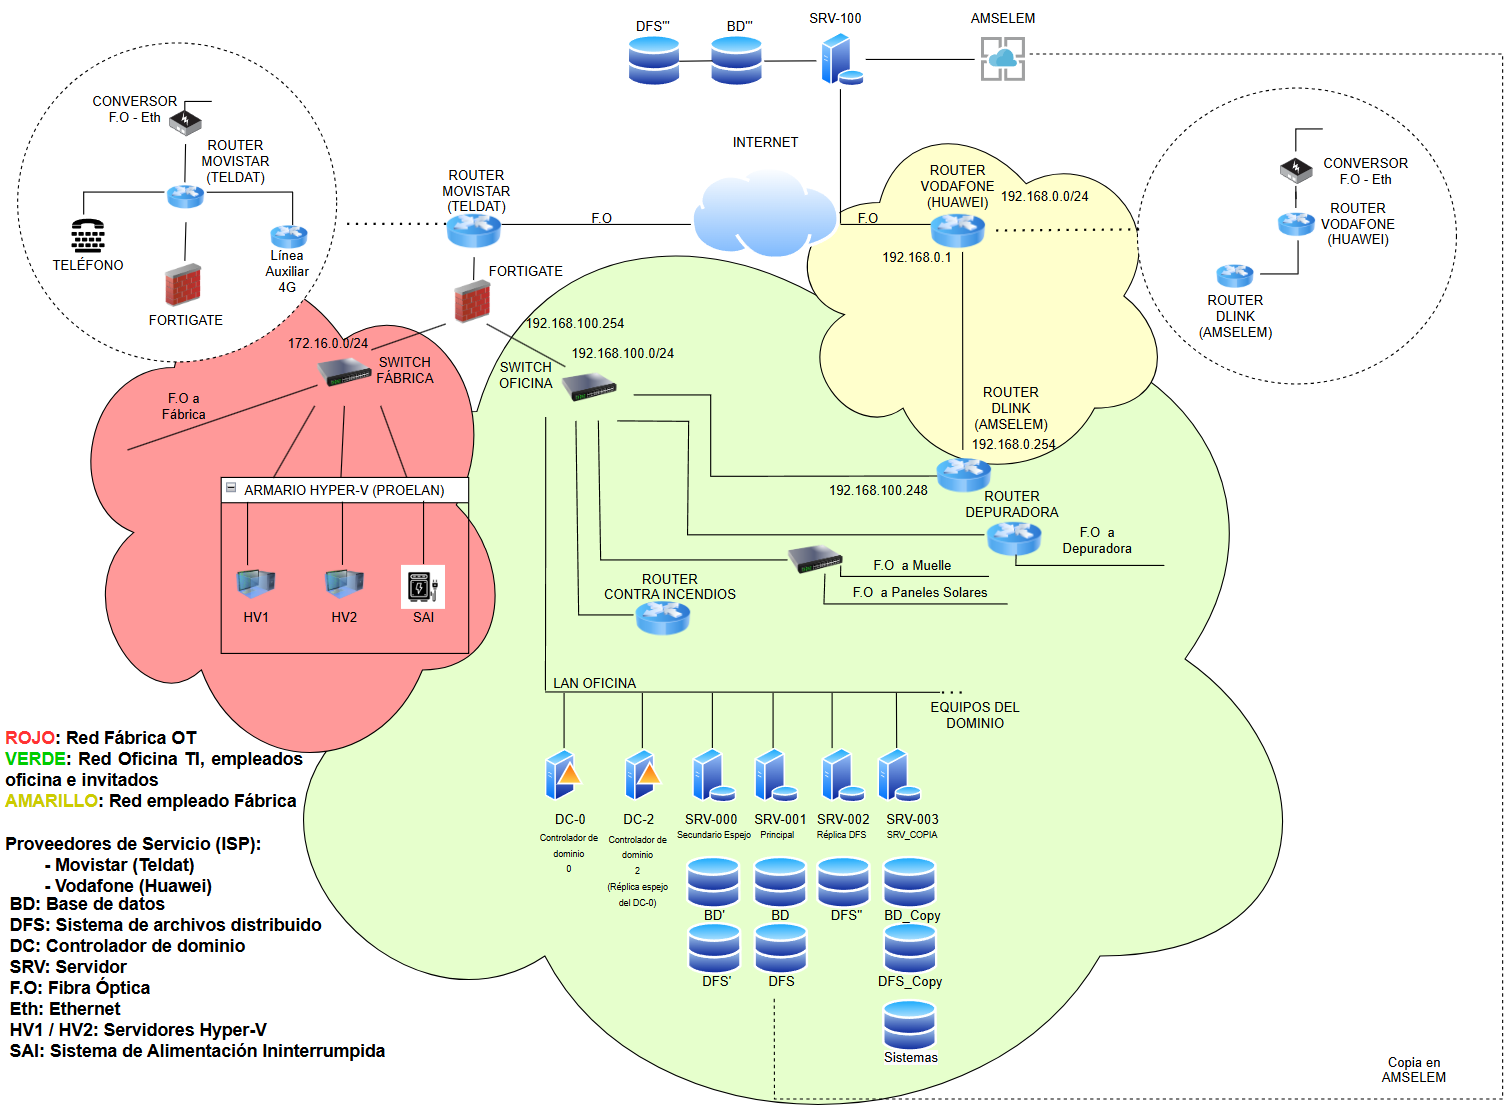
\includegraphics[width=\textwidth]{images/topologia.png}
  \caption{Topología de red de la Empresa X.}
  \label{fig:topologia-red}
\end{figure}

\par\vspace{0.5cm}

Finalmente, con el alcance, herramientas y técnicas claramente definidos, se procedió a preparar todo el material necesario para realizar la auditoría. 
\par\vspace{0.5cm}




\subsubsection{Resultados Obtenidos en la Fase de Planificación}

Como resultado de esta fase de planificación, se lograron concretar los siguientes puntos clave:

\begin{itemize}
    \item Documentos formales firmados por la empresa: acuerdo de confidencialidad (NDA), acuerdo de servicios y autorización para pruebas de pentesting.
    \item Alcance de la auditoría definido claramente en base a la topología de red actualizada.
    \item Actualización completa del inventario de activos en formato Excel.
    \item Elaboración de un diagrama actualizado de la topología de red, entregado formalmente a la empresa.
    \item Reorganización física y propuesta de eliminación de activos obsoletos y equipos no utilizados presentes en las instalaciones.
\end{itemize}



\par\vspace{0.5cm}
\subsection{Fase de Descubrimiento en el Caso Práctico}

Una vez finalizada la fase de planificación, y haber preparado todas las herramientas y autorizaciones necesarias, se procedió con la ejecución de la \textbf{fase de descubrimiento}, según lo establecido en la metodología propuesta de esta memoria.

\par\vspace{0.5cm}

Como paso previo, se llevó a cabo el análisis opcional de OSINT. Esta etapa permitió obtener información pública sobre la organización auditada. En concreto, se localizaron los siguientes elementos relevantes:

\begin{itemize}
    \item Documentos indexados en motores de búsqueda bajo el dominio corporativo
    \item Informes sobre la facturación anual, número de empleados, ejecutivos de la empresa, teléfonos y correos de contactos.
    \item Relaciones internacionales.
    \item Listado de posibles empleados.
    \item Correos corporativos.
    \item Registros de haber sufrido un ciberataque años anteriores.
    \item Inventario de puertos y dominios públicos asociados a la empresa.
\end{itemize}

\par\vspace{0.5cm}

A través de estas búsquedas especializadas, se identificaron varias credenciales asociadas a cuentas corporativas previamente filtradas, lo cual no supone ningún riesgo si llevan a cabo las políticas de cambios de contraseñas, dejando la información expuesto sin ningún valor para un atacante.

\par\vspace{0.5cm}

Tras concluir con el análsiis de OSINT, se inicia formalmente la fase de descubrimiento, se auditó en primer lugar el perímetro inalámbrico de la red, 
siguiendo los procedimientos expuestos en la Sección~\ref{sec:analisis_redes_inalambricas}. 
Para ello se utilizó una antena en modo monitor junto con las herramientas descritas, que permitieron identificar tres redes WiFi vinculadas a la organización. Se observó que dos de ellas compartían el mismo segmento de red, la red de oficina, mientras que la tercera correspondía a una red de invitados, aislada mediante segmentación.

\par\vspace{0.5cm}

Gracias al análisis topológico, pudimos comprobar y evalaur una correcta segmentación mediante un firewall Fortigate de última generación. Las redes identificadas se dividían en un segmento de fábrica (\texttt{172.168.0.0/24}) y uno de oficina (\texttt{192.168.100.0/24}) como se puede ver en la Figura~\ref{fig:topologia-red}. Se evaluó la seguridad de las redes inalámbricas mediante las técnicas de desautenticación descritas en la metodología, obteniéndose los \textit{handshakes} de autenticación para todas las redes detectadas. Estos paquetes fueron almacenados para su posterior análisis en relación con la robustez y complejidad de las contraseñas.

\par\vspace{0.5cm}

A continuación, el responsable de la empresa nos permitió conectarno directamente al segmento de red de la oficina por cable con el fin de agilizar el análisis interno. Se inició una exploración automatizada mediante \texttt{Nessus}, mientras en paralelo se ejecutaban capturas de tráfico con \texttt{Wireshark}. Posteriormente, se utilizó \texttt{Nmap} para enumerar todos los activos.

\par\vspace{0.5cm}

Durante este proceso, algunos escaneos fueron bloqueados por el firewall, lo que obligó a emplear técnicas de evasión y scripts personalizados en \texttt{Python}, uno de los cuales se incluye como ejemplo en el Anexo~\ref{anexo:script_evasion}. Una vez se logró listar los hosts de la red, se procedió a enumerar sus puertos y servicios abiertos de forma individual.

\par\vspace{0.5cm}

Los informes generados por \texttt{Nessus}, junto con los análisis manuales y observaciones realizadas, sirvieron para evaluar las vulnerabilidades detectadas, conforme a la metodología de análisis descrita en la Sección~\ref{sec:analisis_vulnerabilidades}. Esta información permitió sentar las bases para el diseño del posterior plan de ataque.

\par\vspace{0.5cm}

Como resultado directo de esta fase, se obtuvo un conjunto de \textit{handshakes} cuya complejidad será evaluada en base al tiempo estimado de ruptura por fuerza bruta. Asimismo, se generó un inventario detallado de activos, revelando la presencia de un entorno con \textit{Active Directory}, en el cual los nombres de los equipos estaban correctamente etiquetados, facilitando la labor de reconocimiento para un posible atacante.

\par\vspace{0.5cm}

Entre los dispositivos detectados se encontraban routers con paneles de acceso accesibles, servidores de archivos, estaciones de trabajo conectadas al dominio, impresoras de red y dispositivos personales de empleados, como móviles, los cuales representan un potencial vector de riesgo si estuviesen comprometidos. Además, se extrajo un listado preliminar de vulnerabilidades priorizadas para su explotación en fases posteriores.

\par\vspace{0.5cm}


\label{sec:fingerprint}
\label{sec:analisis_vulnerabilidades}
\label{sec:osint}
\label{anexo:script_evasion}
\label{codigo:wireshark}

\par\vspace{0.5cm}

\subsection{Fase de Ataque en el Caso Práctico}


una vezx trazado un plan de ataque adecuado al entorno de directorio activo presenre en la red a aduitar, comenzamos previamtene con el crackero de la contrraseña de la red perimetras, esta era bastante robusta con mas de 10 caracteres combinado numeros letras mayusvcula minuscula y algunas simbolos, por lo que se estima segun la sigueinte tabla: que la duracion para romperla es de .... tiempo.

Nos volvemos a conectar a la red y desde dentro, probamos con un listado de posibles credencales por defecto en todos los paneles de acceso. Durante esta etapa logramos acceder de primera mano a la configuracion como administrado de uno de los routers de la empresa, y acceso como administrador al panel de control de una de las impresoras principales de la red de oficina. Una vez probado con toddos los demas paneles, probamos lo mismo a servicios destinado a la conecxion como es el puerto 22 ssh y otros como el telnet 23. Vimos que todos estaban protegido frente a fuer<za bruta y que contaban con contraseñas. Finalmente, comenzxamos a atacar ese sistme de directorio activo siguiendo la metodologia descrita en la seccion pertinenten arriba del documetno.

Ataque de nessu?
Ataque manuales?
Probamos un shelshock con paneles cgi.


\par\vspace{0.5cm}
\subsection{Fase de Reporte del Caso Práctico}




\clearpage
\thispagestyle{nohead}

% -----------------------------------------------CONCLUSIONES O DISCUSIONES------------------------------------------------------------
\section{Resultados y Conclusiones}

\par\vspace{0.5cm}
\subsection{Líneas de investigación futuras}


\clearpage
\thispagestyle{nohead}

% -----------------------------------------------REFERENCIAS------------------------------------------------------------
%Poner bien las referencias en APA

\section*{Bibliografía}
\addcontentsline{toc}{section}{Bibliografía}
\begin{thebibliography}{99}
    
    \bibitem{napalm-ccoo}
    napalm. (2023, 2 de Diciembre). \textit{Mariscada virtual en el servidor de CCOO} [Entrada de blog]. Recuperado el 8 de Febrero de 2025, de \url{https://defsec.noblogs.org/mariscada-virtual-en-el-servidor-de-ccoo/}

    \bibitem{avtest}
    AV-TEST. (s.f.). \textit{Malware Statistics Portal} [Página web]. Recuperado el 10 de Enero de 2025, de \url{https://portal.av-atlas.org/malware}

    \bibitem{junta-perfiles}
    Ceada Ramos, J. L. (2018, 3 de Agosto). \textit{Informe final sobre la consulta preliminar del mercado: “Perfiles profesionales ámbito informático”} [Informe técnico]. Junta de Andalucía. Recuperado el 13 de Febrero de 2025, de \url{https://www.juntadeandalucia.es/haciendayadministracionpublica/apl/pdc-front-publico/perfiles-licitaciones/consultas-preliminares/detalle?idExpediente=000000078484}

    \bibitem{hiscox}
    Hiscox. (2022, 27 de Junio). \textit{El 44\% de las pymes españolas sufrió al menos un ciberataque durante 2021} [Nota de prensa]. Recuperado el 13 de Febrero de 2025, de \url{https://www.hiscox.es/el-44-de-las-pymes-espanolas-sufrio-al-menos-un-ciberataque-durante-2021}

    \bibitem{incibe2023}
    INCIBE. (2023, 29 de Marzo). \textit{INCIBE gestionó más de 118.000 incidentes de ciberseguridad durante 2022, un 9\% más que en 2021} [Nota de prensa]. Recuperado el 13 de Febrero de 2025, de \url{https://www.incibe.es/incibe/sala-de-prensa/incibe-gestiono-mas-115000-incidentes-ciberseguridad-durante-2022-9-mas}

    \bibitem{pwc}
    PwC España. (2021). \textit{El 86\% de las compañías españolas carecen de una cultura de ciberseguridad entre los empleados} [Nota de prensa]. Recuperado el 13 de Febrero de 2025, de \url{https://www.pwc.es/es/sala-prensa/notas-prensa/2021/companias-espanolas-cultura-ciberseguridad-empleados.html}

    \bibitem{treyder}
    Treyder. (s.f.). \textit{La ciberseguridad en las PYMES: Cómo proteger tu negocio de las amenazas en línea} [Entrada de blog]. Recuperado el 7 de Abril de 2025, de \url{https://www.treyder.com/blog/ciberseguridad-en-las-pymes/}

    \bibitem{vuln}
    Morales-López \& Taipe-Yanez \& Pallo-Tulmo, (2024) \textit{Estrategias de Auditoría en ciberseguridad y su importancia en las empresas una revisión bibliográfica} Recuperado el 07 de Abril de 2025, de \url{https://www.investigarmqr.com/ojs/index.php/mqr/article/view/1436/4849}

    \bibitem{toms2021}
    Toms, L. (2021, 30 de Julio). \textit{5 riesgos de seguridad para las PYMEs que se deben tener en cuenta}. GlobalSign. Recuperado el 7 de Abril de 2025, de \href{https://www.globalsign.com/es/blog/top-5-pequena-empresa-grandes-riesgos-5-riesgos-de-seguridad-para-las-pymes-que-se-deben-tener-en-cuenta}{https://www.globalsign.com/es/blog/} 
        
    \bibitem{fortinet}
    Fortinet. (s.f.). \textit{Threat Map} [Mapa interactivo]. Recuperado el 7 de Abril de 2025, de \url{https://fortiguard.fortinet.com/threat-map}

    \bibitem{mitigacion}
    Viteri-Hernández, C., \& Avila-Pesantez, D. (2024). \textit{Exploración integral de la seguridad en redes de proveedores de servicios de Internet: Una revisión sistemática de literatura}. Recuperado el 5 de Mayo de 2025, de \url{https://perspectivas.espoch.edu.ec/RCP_ESPOCH/article/view/215/146}
        
    \bibitem{incibe}
    INCIBE. (2015, 4 de Diciembre). \textit{Introducción a INCIBE} [Video]. Recuperado el 24 de Mayo de 2025, de \url{https://www.youtube.com/watch?v=zFCq191o1oA}

    \bibitem{cni}
    Centro Nacional de Inteligencia. (s.f.). \textit{Objetivos y valores}. Recuperado el 24 de Mayo de 2025, de \url{https://www.cni.es/sobre-el-cni/objetivos-y-valores}

    \bibitem{ccncert}
    Centro Criptológico Nacional (CCN-CERT). (s.f.). \textit{Portal del CCN-CERT}. Recuperado el 24 de Mayo de 2025, de \url{https://www.ccn-cert.cni.es/es/sobre-nosotros/}

    \bibitem{aepd}
    Agencia Española de Protección de Datos (AEPD). (2024, 13 de Marzo). \textit{Portal de la AEPD}. Recuperado el 24 de Mayo de 2025, de \url{https://www.aepd.es/la-agencia/transparencia/informacion-de-caracter-institucional-organizativa-y-de-planificacion-0}

    \bibitem{nist}
    National Institute of Standards and Technology (NIST). (s.f.). \textit{Cybersecurity Framework}. Recuperado el 24 de Mayo de 2025, de \url{https://www.nist.gov/about-nist}

    \bibitem{device42}
    Device42. (2024). \textit{NIST CSF Categories: Description, Examples, and Best Practices}. Recuperado el 24 de Mayo de 2025, de \url{https://www.device42.com/compliance-standards/nist-csf-categories/}

    \bibitem{nistsp}
    SEGURIDAD CERO (2022, 26 de Mayo). \textit{Ciberseguridad Buenas Practicas | NIST} [Video]. Recuperado el 24 de Mayo de 2025, de \url{https://www.youtube.com/watch?v=i3McVotWrl8&t=718s&ab_channel=SEGURIDADCERO}

    \bibitem{sans}
    SANS Institute. (s.f.). \textit{SANS Cyber Security Training and Certifications}. Recuperado el 25 de Mayo de 2025, de \url{https://www.sans.org/}

    \bibitem{sanscert}
    SANS Institute. (s.f.). \textit{Red Team Operations Certifications}. Recuperado el 25 de Mayo de 2025, de \url{https://www.giac.org/focus-areas/offensive-operations/}

    \bibitem{boe_ens}
    Centro Criptológico Nacional (CCN-CERT). (s.f). \textit{Esquema Nacional de Seguridad (ENS)}. Recuperado el 26 de Mayo de 2025, de \url{https://ens.ccn.cni.es/es/que-es-el-ens/faq}

    \bibitem{rgpd}
    Agencia Española de Protección de Datos (AEPD) (s.f). \textit{Reglamento General de Protección de Datos (RGPD)}. Recuperado el 26 de Mayo de 2025, de \url{https://ens.ccn.cni.es/es/que-es-el-ens}

    \bibitem{boe_lopdgdd}
    Boletín Oficial del Estado. (2018). \textit{Ley Orgánica 3/2018, de Protección de Datos Personales y garantía de los derechos digitales}. Recuperado el 26 de Mayo de 2025, de \url{https://www.boe.es/eli/es/lo/2018/12/05/3}

    \bibitem{nis2}
    Ingertec. (s.f.). \textit{Directiva NIS 2}. Recuperado el 28 de Mayo de 2025, de \url{https://ingertec.com/ciberseguridad/directiva-nis-2/}

    \bibitem{iso27001}
    International Organization for Standardization. (s.f). \textit{NORMA ISO 27001}. Recuperado el 28 de Mayo de 2025, de \url{https://www.normaiso27001.es/}

    \bibitem{triada}
    4IT Networks. (s.f.). \textit{Seguridad y Protección de la Información}. Recuperado el 28 de Mayo de 2025, de \url{https://www.4itn.mx/ciberseguridad/}

    \bibitem{owasp}
    OWASP Foundation. (s.f.). \textit{Open Web Application Security Project}. Recuperado el 22 de Mayo de 2025, de \url{https://owasp.org/about/}

    \bibitem{osstmm}
    ISECOM. (s.f.). \textit{OSSTMM – Open Source Security Testing Methodology Manual}. Recuperado el 22 de Mayo de 2025, de \url{https://www.isecom.org/OSSTMM.3.pdf}

    \bibitem{tibereu}
    European Central Bank. (s.f.). \textit{TIBER-EU Framework}. Recuperado el 22 de Mayo de 2025, de \url{https://www.ecb.europa.eu/pub/pdf/other/ecb.tiber_eu_framework.en.pdf}

    \bibitem{nist80053}
    National Institute of Standards and Technology. (2020). \textit{NIST Special Publication 800-53 Revision 5: Security and Privacy Controls for Information Systems and Organizations}. Recuperado el 22 de Mayo de 2025, de \url{https://doi.org/10.6028/NIST.SP.800-53r5}

    \bibitem{nist800115}
    Scarfone, K., Souppaya, M., Cody, A., \& Orebaugh, A. (2008). \textit{Technical guide to information security testing and assessment (NIST SP 800-115)}. National Institute of Standards and Technology. Recuperado el 22 de Mayo de 2025, de \url{https://doi.org/10.6028/NIST.SP.800-115}

    \bibitem{beehacker}
    BeeHackers. (s.f.). \textit{BeeHackers}. [Página Web] Recuperado el 7 de junio de 2025, de \url{https://beehackers.es/}

    \bibitem{felipe2024}
    Felipe Redondo, A. M., \& Núñez Cárdenas, F. J. (2024). \textit{Criterios de selección de herramientas para pentesting}. \textit{Artículo Científico}. Recuperado el 8 de Abril de 2025, de \url{https://repository.uaeh.edu.mx/revistas/index.php/huejutla/article/view/12763/11251}

    \bibitem{cvss}
    FIRST. (s.f.). \textit{Common Vulnerability Scoring System}. Recuperado el 7 de Junio de 2025, de \url{https://www.first.org/cvss/specification-document}

    \bibitem{nist80030}
    National Institute of Standards and Technology. (2012). \textit{Guide for conducting risk assessments}.  Recuperado el 07 de Junio de 2025, de \url{https://nvlpubs.nist.gov/nistpubs/Legacy/SP/nistspecialpublication800-30r1.pdf}


\end{thebibliography}


\clearpage







% -----------------------------------------------ANEXOS------------------------------------------------------------
\thispagestyle{nohead}


\section*{Anexo 1. Registro de actividades en Clockify}
\addcontentsline{toc}{section}{Anexo 1}

\label{anexo:1}

A continuación se muestra el enlace al recurso utilizado para el control del tiempo y la gestión de tareas del proyecto. Este recurso, gestionado a través de la plataforma Clockify, recoge de forma detallada todas las actividades realizadas durante el desarrollo del TFG. 

El registro incluye:
\begin{itemize}
  \item El total de horas dedicadas al desarrollo del proyecto.
  \item Las fechas y horas dedicadas a cada tarea.
  \item Las actividades clasificadas según las fases establecidas en el cronograma.
  \item Una breve descripción para cada actividad desarrollada.
\end{itemize}

\begin{tcolorbox}[enhanced,attach boxed title to top center={yshift=-3mm,yshifttext=-1mm},
  colback=blue!5!white,colframe=blue!75!black,colbacktitle=red!80!black,
  title=Dirección URL,fonttitle=\bfseries,
  boxed title style={size=small,colframe=red!50!black} ]
  \centering
  \url{https://app.clockify.me/shared/abc123}

\end{tcolorbox}


\clearpage

\thispagestyle{nohead}


\section*{Anexo 2. Enlaces oficiales de herramientas de pentesting}
\label{anexo:2}
\addcontentsline{toc}{section}{Anexo 2}

\subsection*{Sistemas Operativos}
\begin{table}[H]
\centering
\begin{tabular}{|m{5cm}|m{10cm}|}
\hline
\textbf{Herramienta} & \textbf{URL} \\
\hline
Kali Linux & \url{https://www.kali.org} \\
\hline
Parrot OS & \url{https://www.parrotsec.org} \\
\hline
\end{tabular}
\end{table}

\subsection*{Herramientas OSINT}
\begin{table}[H]
\centering
\begin{tabular}{|m{5cm}|m{10cm}|}
\hline
\textbf{Herramienta} & \textbf{URL} \\
\hline
Shodan & \url{https://www.shodan.io} \\
\hline
Censys & \url{https://censys.io} \\
\hline
TheHarvester & \url{https://github.com/laramies/theHarvester} \\
\hline
Maltego & \url{https://www.maltego.com} \\
\hline
\end{tabular}
\end{table}

\subsection*{Herramientas de Enumeración y Escaneo}
\begin{table}[H]
\centering
\begin{tabular}{|m{5cm}|m{10cm}|}
\hline
\textbf{Herramienta} & \textbf{URL} \\
\hline
Nmap & \url{https://nmap.org} \\
\hline
Nessus & \url{https://www.tenable.com/products/nessus} \\
\hline
SQLmap & \url{https://sqlmap.org} \\
\hline
OpenVAS (Greenbone) & \url{https://www.greenbone.net/en/} \\
\hline
Nikto & \url{https://github.com/sullo/nikto} \\
\hline
\end{tabular}
\end{table}

\subsection*{Herramientas para Aplicaciones Web}
\begin{table}[H]
\centering
\begin{tabular}{|m{5cm}|m{10cm}|}
\hline
\textbf{Herramienta} & \textbf{URL} \\
\hline
Burp Suite & \url{https://portswigger.net/burp} \\
\hline
ZAP (Zed Attack Proxy) & \url{https://www.zaproxy.org} \\
\hline
\end{tabular}
\end{table}

\subsection*{Herramientas para Auditoría de Redes Wi-Fi}
\begin{table}[H]
\centering
\begin{tabular}{|m{5cm}|m{10cm}|}
\hline
\textbf{Herramienta} & \textbf{URL} \\
\hline
Aircrack-ng & \url{https://www.aircrack-ng.org} \\
\hline
Wifi Pineapple & \url{https://shop.hak5.org/collections/2025-best-sellers/products/wifi-pineapple-enterprise} \\
\hline
\end{tabular}
\end{table}

\subsection*{Herramientas Físicas (Hardware Hacking)}
\begin{table}[H]
\centering
\begin{tabular}{|m{5cm}|m{10cm}|}
\hline
\textbf{Herramienta} & \textbf{URL} \\
\hline
Flipper Zero & \url{https://flipperzero.one} \\
\hline
USB Rubber Ducky & \url{https://shop.hak5.org/products/usb-rubber-ducky-deluxe} \\
\hline
\end{tabular}
\end{table}

\subsection*{Post-Explotación y Explotación}
\begin{table}[H]
\centering
\begin{tabular}{|m{5cm}|m{10cm}|}
\hline
\textbf{Herramienta} & \textbf{URL} \\
\hline
Metasploit & \url{https://www.metasploit.com} \\
\hline
John the Ripper & \url{https://www.openwall.com/john} \\
\hline
BloodHound & \url{https://github.com/BloodHoundAD/BloodHound} \\
\hline
NetExec (antes CrackMapExec) & \url{https://github.com/Pennyw0rth/NetExec} \\
\hline
Mimikatz & \url{https://github.com/gentilkiwi/mimikatz} \\
\hline
\end{tabular}
\end{table}

\subsection*{Análisis de Tráfico de Red}
\begin{table}[H]
\centering
\begin{tabular}{|m{5cm}|m{10cm}|}
\hline
\textbf{Herramienta} & \textbf{URL} \\
\hline
Wireshark & \url{https://www.wireshark.org} \\
\hline
\end{tabular}
\end{table}


\clearpage
\thispagestyle{nohead}

\section*{Anexo 3: Glosario de términos}
\label{anexo:3}
\addcontentsline{toc}{section}{Anexo 3}

A continuación se presenta un glosario con los principales términos utilizados en el presente trabajo:

\begin{itemize}

    \item \textbf{AD}: Active Directory. Servicio de directorio desarrollado por Microsoft para gestionar usuarios, equipos y recursos en una red.

    \item \textbf{AEPD}: Agencia Española de Protección de Datos. Autoridad nacional encargada de velar por el cumplimiento del RGPD y la LOPD-GDD en España.

    \item \textbf{AP}: Access Point (Punto de acceso). Dispositivo que permite la conexión de dispositivos inalámbricos a una red cableada.

    \item \textbf{APA}: American Psychological Association. Estilo de citación utilizado habitualmente en ciencias sociales y documentos académicos.

    \item \textbf{API}: Application Programming Interface. Conjunto de funciones que permite la comunicación entre diferentes aplicaciones o servicios.

    \item \textbf{ARP}: Address Resolution Protocol. Protocolo que asocia direcciones IP con direcciones MAC en redes locales.

    \item \textbf{BLE}: Bluetooth Low Energy. Versión de bajo consumo del estándar Bluetooth, usado en dispositivos IoT y móviles.

    \item \textbf{BSSID}: Basic Service Set Identifier. Dirección MAC única del punto de acceso Wi-Fi.

    \item \textbf{CCN-CERT}: Capacidad de Respuesta a Incidentes del Centro Criptológico Nacional. Organismo especializado en ciberseguridad y respuesta a amenazas en la administración pública.

    \item \textbf{CIDR}: Classless Inter-Domain Routing. Notación para representar rangos de direcciones IP mediante una dirección seguida de una barra y el número de bits de red (ej. \texttt{/24}).

    \item \textbf{CISO}: Chief Information Security Officer. Directivo encargado de definir y supervisar la estrategia de ciberseguridad de una organización.

    \item \textbf{CMD}: Command. Abreviatura común para referirse a la línea de comandos o terminal.

    \item \textbf{CoAP}: Constrained Application Protocol. Protocolo optimizado para dispositivos IoT con recursos limitados.

    \item \textbf{CNI}: Centro Nacional de Inteligencia. Agencia de inteligencia española con competencias en seguridad del Estado.

    \item \textbf{CSRF}: Cross-Site Request Forgery. Ataque que hace que un usuario autenticado ejecute acciones no deseadas en una aplicación web.

    \item \textbf{CTO}: Chief Technology Officer. Responsable de la estrategia tecnológica y del liderazgo en innovación dentro de una organización.

    \item \textbf{CVE}: Common Vulnerabilities and Exposures. Identificador estándar para vulnerabilidades conocidas en software y hardware.

    \item \textbf{DDoS}: Distributed Denial of Service. Ataque que busca colapsar un sistema mediante el envío masivo de tráfico desde múltiples fuentes.

    \item \textbf{DNS}: Domain Name System. Sistema que traduce nombres de dominio legibles por humanos a direcciones IP.

    \item \textbf{EE}: Entorno Empresarial. Conjunto de condiciones externas e internas que afectan a la actividad de una empresa.

    \item \textbf{EI}: Entorno Interno. Factores y recursos propios de una organización que influyen en su gestión y seguridad.

    \item \textbf{ENS}: Esquema Nacional de Seguridad. Marco normativo español que establece requisitos de seguridad para sistemas de las administraciones públicas.

    \item \textbf{GHDB}: Google Hacking Database. Base de datos de búsquedas avanzadas que pueden revelar información sensible mediante motores de búsqueda.

    \item \textbf{GIAC}: Global Information Assurance Certification. Conjunto de certificaciones profesionales en seguridad de la información emitidas por SANS.

    \item \textbf{GPO}: Group Policy Object. Conjunto de reglas en sistemas Windows que controlan la configuración de usuarios y equipos.

    \item \textbf{HTTP}: HyperText Transfer Protocol. Protocolo utilizado para la transferencia de datos en la web.

    \item \textbf{IDOR}: Insecure Direct Object Reference. Vulnerabilidad que permite acceder a recursos sin autorización mediante manipulación de identificadores.

    \item \textbf{IDS/IPS}: Intrusion Detection/Prevention System. Sistemas para detectar (IDS) y prevenir (IPS) accesos o actividades maliciosas en una red.

    \item \textbf{INCIBE}: Instituto Nacional de Ciberseguridad. Organismo español encargado de impulsar la ciberseguridad en ciudadanos, empresas y operadores estratégicos.

    \item \textbf{IoT}: Internet of Things. Red de dispositivos físicos conectados a internet que recopilan y comparten datos.

    \item \textbf{ISO/IEC}: Conjunto de estándares internacionales de la Organización Internacional de Normalización y la Comisión Electrotécnica Internacional.

    \item \textbf{LOPD-GDD}: Ley Orgánica de Protección de Datos y Garantía de Derechos Digitales. Ley española que adapta el RGPD al marco legal nacional.

    \item \textbf{MFA}: Multi-Factor Authentication. Sistema de autenticación que requiere más de un factor (como contraseña y código enviado al móvil) para verificar la identidad de un usuario.

    \item \textbf{MITM}: Man-In-The-Middle. Ataque en el que un tercero intercepta y/o modifica las comunicaciones entre dos partes sin que estas lo sepan.

    \item \textbf{MQTT}: Message Queuing Telemetry Transport. Protocolo ligero para la comunicación entre dispositivos IoT.

    \item \textbf{NDA}: Non-Disclosure Agreement (Acuerdo de confidencialidad). Contrato legal que obliga a las partes a no divulgar información sensible o confidencial.

    \item \textbf{NIST}: National Institute of Standards and Technology. Organismo estadounidense que publica estándares y guías de ciberseguridad de referencia internacional.

    \item \textbf{OS}: Operating System. Software principal que gestiona el hardware y recursos de un sistema.

    \item \textbf{OSINT}: Open Source Intelligence. Recopilación de información a partir de fuentes públicas como parte del proceso de análisis o investigación.

    \item \textbf{OSSTMM}: Open Source Security Testing Methodology Manual. Marco metodológico abierto para auditorías de seguridad y evaluación de riesgos.

    \item \textbf{OT}: Operational Technology. Tecnología utilizada para el control de procesos físicos (como maquinaria industrial), distinta de la TI tradicional.

    \item \textbf{OWASP}: Open Web Application Security Project. Proyecto abierto que promueve buenas prácticas y recursos para mejorar la seguridad de las aplicaciones web.

    \item \textbf{Pymes}: Pequeñas y Medianas Empresas. Negocios con limitaciones de recursos humanos y económicos en comparación con grandes corporaciones.

    \item \textbf{Protocolos}: Conjunto de reglas que rigen la comunicación entre dispositivos en una red (ej. HTTP, FTP, TCP/IP).

    \item \textbf{PTES}: Penetration Testing Execution Standard. Estándar que define buenas prácticas y metodologías para realizar pruebas de penetración (pentesting).

    \item \textbf{RCE}: Remote Code Execution. Vulnerabilidad que permite ejecutar código malicioso de forma remota en un sistema comprometido.

    \item \textbf{RGPD}: Reglamento General de Protección de Datos. Normativa europea que regula el tratamiento de datos personales y garantiza los derechos de los ciudadanos.

    \item \textbf{SANS}: SysAdmin, Audit, Network and Security. Organización líder en formación y certificación en ciberseguridad.

    \item \textbf{SGSI}: Sistema de Gestión de Seguridad de la Información. Conjunto de políticas, procedimientos y controles diseñados para proteger los activos de información.

    \item \textbf{SMS}: Short Message Service. Servicio de mensajería de texto utilizado también como segundo factor de autenticación.

    \item \textbf{SQL}: Structured Query Language. Lenguaje utilizado para gestionar bases de datos, a menudo objetivo de ataques como la inyección SQL.

    \item \textbf{SQLi}: SQL Injection. Ataque que consiste en insertar comandos SQL maliciosos en formularios o URLs para manipular bases de datos.

    \item \textbf{SSH}: Secure Shell. Protocolo de red que permite la administración remota segura de sistemas.

    \item \textbf{SSID}: Service Set Identifier. Nombre que identifica una red Wi-Fi.

    \item \textbf{SUID}: Set User ID. Permiso especial en sistemas Unix que permite ejecutar un archivo con los privilegios del propietario.

    \item \textbf{TFG}: Trabajo de Fin de Grado. Proyecto académico obligatorio para la obtención del título universitario de grado.

    \item \textbf{TIBER}: Threat Intelligence-Based Ethical Red Teaming. Marco europeo para realizar ejercicios avanzados de simulación de ciberataques en infraestructuras críticas.

    \item \textbf{TI}: Tecnologías de la Información. Conjunto de recursos tecnológicos utilizados para gestionar y procesar información.

    \item \textbf{TOR}: The Onion Router. Red diseñada para navegar de forma anónima a través de múltiples capas de cifrado.

    \item \textbf{UE}: Unión Europea. Comunidad política y económica que agrupa a 27 países europeos, responsable de normativas como el RGPD.

    \item \textbf{UPnP}: Universal Plug and Play. Conjunto de protocolos que permite la conexión automática de dispositivos en una red.

    \item \textbf{VLAN}: Virtual LAN. Red lógica que segmenta dispositivos dentro de una misma red física para mejorar la seguridad y eficiencia.

    \item \textbf{VPN}: Virtual Private Network. Red privada virtual que cifra la conexión a internet para proteger la privacidad y seguridad.

    \item \textbf{WAF}: Web Application Firewall. Sistema de seguridad que protege aplicaciones web contra ataques como XSS o SQLi.

    \item \textbf{WEP}: Wired Equivalent Privacy. Protocolo de seguridad obsoleto para redes Wi-Fi, vulnerable a múltiples ataques.

    \item \textbf{WPA}: Wi-Fi Protected Access. Protocolo de seguridad para redes inalámbricas, sucesor de WEP.

    \item \textbf{XSS}: Cross-Site Scripting. Vulnerabilidad que permite inyectar scripts maliciosos en páginas web vistas por otros usuarios.

    \item \textbf{XXE}: XML External Entity. Vulnerabilidad que permite a un atacante acceder a archivos o recursos internos a través de procesamiento inseguro de XML.
\end{itemize}

\clearpage
\thispagestyle{nohead}

\section*{Anexo 4: Parámetros avanzados de Nmap}
\label{anexo:4}
\addcontentsline{toc}{section}{Anexo 4}

Dado el papel fundamental que desempeña \textbf{Nmap} en las tareas de reconocimiento durante una auditoría de ciberseguridad, a continuación se sintetizan sus funcionalidades más relevantes mediante el uso de parámetros específicos según el tipo de análisis requerido.

\vspace{1em}

\begin{table}[H]
\centering
\renewcommand{\arraystretch}{1.3}
\begin{tabularx}{\textwidth}{clXc}
\toprule
\textbf{Parámetro} & \textbf{} & \textbf{Función} & \textbf{Categoría} \\
\midrule
\bottomrule
\texttt{-sn} & & Realiza un escaneo sin comprobar puertos (ping scan). Detecta si los hosts están activos. & Detección de hosts \\
\bottomrule
\texttt{-sS} & & Escaneo SYN (stealth scan). No completa la conexión TCP (half-open). & Sigilo \\
\bottomrule
\texttt{-sT} & & Escaneo TCP completo con conexión. Útil si no se tienen privilegios root. & Estándar \\
\bottomrule
\texttt{-sU} & & Escaneo de puertos UDP. Más lento pero detecta servicios no-TCP. & Cobertura total \\
\bottomrule
\texttt{-Pn} & & Desactiva el ping inicial (asume que los hosts están activos). Evita bloqueos por firewall. & Evasión \\
\bottomrule
\texttt{-f}  & & Fragmenta los paquetes para dificultar su detección por sistemas IDS/IPS. & Evasión \\
\bottomrule
\texttt{-D decoy1,decoy2} & & Usa direcciones señuelo (decoys) para ocultar la IP real del escáner. & Evasión \\
\bottomrule
\texttt{-T0} -- \texttt{-T5} & & Controla la velocidad y agresividad del escaneo. `T0` es muy lento/sigiloso, `T5` es muy rápido. & Rendimiento / Sigilo \\
\bottomrule
\texttt{-sV} & & Detecta versiones de servicios en puertos abiertos. & Identificación \\
\bottomrule
\texttt{-O} & & Intenta identificar el sistema operativo del host. & Identificación \\
\bottomrule
\texttt{-A} & & Realiza detección avanzada: SO, versiones, traceroute y scripts NSE. & Detección avanzada \\
\bottomrule
\texttt{-n} & & Desactiva la resolución DNS para aumentar la velocidad. & Rendimiento \\
\bottomrule
\texttt{-v}, \texttt{-vv} & & Aumenta el nivel de detalle (verbose) en la salida del escaneo. & Monitorización \\
\bottomrule
\texttt{-oA base} & & Guarda los resultados en tres formatos: XML, normal y grepable. & Registro \\
\bottomrule
\end{tabularx}
\caption{Parámetros avanzados de Nmap clasificados por funcionalidad}
\label{tab:nmap_avanzado}
\end{table}



\end{document}